%% $Id$
\documentclass[12pt]{report}
\usepackage{graphicx,a4,latexsym,../pdfsetup}

\makeatletter
%	proof.sty	(Proof Figure Macros)
%
% 	version 1.0
%	October 13, 1990
% 	Copyright (C) 1990 Makoto Tatsuta (tatsuta@riec.tohoku.ac.jp)
% 
% This program is free software; you can redistribute it or modify
% it under the terms of the GNU General Public License as published by
% the Free Software Foundation; either versions 1, or (at your option)
% any later version.
% 
% This program is distributed in the hope that it will be useful
% but WITHOUT ANY WARRANTY; without even the implied warranty of
% MERCHANTABILITY or FITNESS FOR A PARTICULAR PURPOSE.  See the
% GNU General Public License for more details.
%
%	Usage:
%		In \documentstyle, specify an optional style `proof', say,
%			\documentstyle[proof]{article}.
%
%	The following macros are available:
%
%	In all the following macros, all the arguments such as
%	<Lowers> and <Uppers> are processed in math mode.
%
%	\infer<Lower><Uppers>
%		draws an inference.
%
%		Use & in <Uppers> to delimit upper formulae.
%		<Uppers> consists more than 0 formulae.
%
%		\infer returns \hbox{ ... } or \vbox{ ... } and
%		sets \@LeftOffset and \@RightOffset globally.
%
%	\infer[<Label>]<Lower><Uppers>
%		draws an inference labeled with <Label>.
%
%	\infer*<Lower><Uppers>
%		draws a many step deduction.
%
%	\infer*[<Label>]<Lower><Uppers>
%		draws a many step deduction labeled with <Label>.
%
%	\deduce<Lower><Uppers>
%		draws an inference without a rule.
%
%	\deduce[<Proof>]<Lower><Uppers>
%		draws a many step deduction with a proof name.
%
%	Example:
%		If you want to write
%       	       	    B C
%		 	   -----
%		       A     D
%		      ----------
%			  E
%	use
%		\infer{E}{
%			A
%			&
%			\infer{D}{B & C}
%		}
%

%	Style Parameters

\newdimen\inferLineSkip		\inferLineSkip=2pt
\newdimen\inferLabelSkip	\inferLabelSkip=5pt
\def\inferTabSkip{\quad}

%	Variables

\newdimen\@LeftOffset	% global
\newdimen\@RightOffset	% global
\newdimen\@SavedLeftOffset	% safe from users

\newdimen\UpperWidth
\newdimen\LowerWidth
\newdimen\LowerHeight
\newdimen\UpperLeftOffset
\newdimen\UpperRightOffset
\newdimen\UpperCenter
\newdimen\LowerCenter
\newdimen\UpperAdjust
\newdimen\RuleAdjust
\newdimen\LowerAdjust
\newdimen\RuleWidth
\newdimen\HLabelAdjust
\newdimen\VLabelAdjust
\newdimen\WidthAdjust

\newbox\@UpperPart
\newbox\@LowerPart
\newbox\@LabelPart
\newbox\ResultBox

%	Flags

\newif\if@inferRule	% whether \@infer draws a rule.
\newif\if@ReturnLeftOffset	% whether \@infer returns \@LeftOffset.
\newif\if@MathSaved	% whether inner math mode where \infer or
			% \deduce appears.

%	Special Fonts

\def\DeduceSym{\vtop{\baselineskip4\p@ \lineskiplimit\z@
    \vbox{\hbox{.}\hbox{.}\hbox{.}}\hbox{.}}}

%	Math Save Macros
%
%	\@SaveMath is called in the very begining of toplevel macros
%	which are \infer and \deduce.
%	\@RestoreMath is called in the very last before toplevel macros end.
%	Remark \infer and \deduce ends calling \@infer.

\def\@SaveMath{\@MathSavedfalse \ifmmode \ifinner
	\relax $\relax \@MathSavedtrue \fi\fi }

\def\@RestoreMath{\if@MathSaved \relax $\relax\fi }

%	Macros

\def\@ifEmpty#1#2#3{\def\@tempa{\@empty}\def\@tempb{#1}\relax
	\ifx \@tempa \@tempb #2\else #3\fi }

\def\infer{\@SaveMath \@ifnextchar *{\@inferSteps}{\@inferOneStep}}

\def\@inferOneStep{\@inferRuletrue
	\@ifnextchar [{\@infer}{\@infer[\@empty]}}

\def\@inferSteps*{\@ifnextchar [{\@@inferSteps}{\@@inferSteps[\@empty]}}

\def\@@inferSteps[#1]{\@deduce{#1}[\DeduceSym]}

\def\deduce{\@SaveMath \@ifnextchar [{\@deduce{\@empty}}
	{\@inferRulefalse \@infer[\@empty]}}

%	\@deduce<Proof Label>[<Proof>]<Lower><Uppers>

\def\@deduce#1[#2]#3#4{\@inferRulefalse
	\@infer[\@empty]{#3}{\@SaveMath \@infer[{#1}]{#2}{#4}}}

%	\@infer[<Label>]<Lower><Uppers>
%		If \@inferRuletrue, draws a rule and <Label> is right to
%		a rule.
%		Otherwise, draws no rule and <Label> is right to <Lower>.

\def\@infer[#1]#2#3{\relax
% Get parameters
	\if@ReturnLeftOffset \else \@SavedLeftOffset=\@LeftOffset \fi
	\setbox\@LabelPart=\hbox{$#1$}\relax
	\setbox\@LowerPart=\hbox{$#2$}\relax
%
	\global\@LeftOffset=0pt
	\setbox\@UpperPart=\vbox{\tabskip=0pt \halign{\relax
		\global\@RightOffset=0pt \@ReturnLeftOffsettrue $##$&&
		\inferTabSkip
		\global\@RightOffset=0pt \@ReturnLeftOffsetfalse $##$\cr
		#3\cr}}\relax
%			Here is a little trick.
%			\@ReturnLeftOffsettrue(false) influences on \infer or
%			\deduce placed in ## locally
%			because of \@SaveMath and \@RestoreMath.
	\UpperLeftOffset=\@LeftOffset
	\UpperRightOffset=\@RightOffset
% Calculate Adjustments
	\LowerWidth=\wd\@LowerPart
	\LowerHeight=\ht\@LowerPart
	\LowerCenter=0.5\LowerWidth
%
	\UpperWidth=\wd\@UpperPart \advance\UpperWidth by -\UpperLeftOffset
	\advance\UpperWidth by -\UpperRightOffset
	\UpperCenter=\UpperLeftOffset
	\advance\UpperCenter by 0.5\UpperWidth
%
	\ifdim \UpperWidth > \LowerWidth
		% \UpperCenter > \LowerCenter
	\UpperAdjust=0pt
	\RuleAdjust=\UpperLeftOffset
	\LowerAdjust=\UpperCenter \advance\LowerAdjust by -\LowerCenter
	\RuleWidth=\UpperWidth
	\global\@LeftOffset=\LowerAdjust
%
	\else	% \UpperWidth <= \LowerWidth
	\ifdim \UpperCenter > \LowerCenter
%
	\UpperAdjust=0pt
	\RuleAdjust=\UpperCenter \advance\RuleAdjust by -\LowerCenter
	\LowerAdjust=\RuleAdjust
	\RuleWidth=\LowerWidth
	\global\@LeftOffset=\LowerAdjust
%
	\else	% \UpperWidth <= \LowerWidth
		% \UpperCenter <= \LowerCenter
%
	\UpperAdjust=\LowerCenter \advance\UpperAdjust by -\UpperCenter
	\RuleAdjust=0pt
	\LowerAdjust=0pt
	\RuleWidth=\LowerWidth
	\global\@LeftOffset=0pt
%
	\fi\fi
% Make a box
	\if@inferRule
%
	\setbox\ResultBox=\vbox{
		\moveright \UpperAdjust \box\@UpperPart
		\nointerlineskip \kern\inferLineSkip
		\moveright \RuleAdjust \vbox{\hrule width\RuleWidth}\relax
		\nointerlineskip \kern\inferLineSkip
		\moveright \LowerAdjust \box\@LowerPart }\relax
%
	\@ifEmpty{#1}{}{\relax
%
	\HLabelAdjust=\wd\ResultBox	\advance\HLabelAdjust by -\RuleAdjust
	\advance\HLabelAdjust by -\RuleWidth
	\WidthAdjust=\HLabelAdjust
	\advance\WidthAdjust by -\inferLabelSkip
	\advance\WidthAdjust by -\wd\@LabelPart
	\ifdim \WidthAdjust < 0pt \WidthAdjust=0pt \fi
%
	\VLabelAdjust=\dp\@LabelPart
	\advance\VLabelAdjust by -\ht\@LabelPart
	\VLabelAdjust=0.5\VLabelAdjust	\advance\VLabelAdjust by \LowerHeight
	\advance\VLabelAdjust by \inferLineSkip
%
	\setbox\ResultBox=\hbox{\box\ResultBox
		\kern -\HLabelAdjust \kern\inferLabelSkip
		\raise\VLabelAdjust \box\@LabelPart \kern\WidthAdjust}\relax
%
	}\relax % end @ifEmpty
%
	\else % \@inferRulefalse
%
	\setbox\ResultBox=\vbox{
		\moveright \UpperAdjust \box\@UpperPart
		\nointerlineskip \kern\inferLineSkip
		\moveright \LowerAdjust \hbox{\unhbox\@LowerPart
			\@ifEmpty{#1}{}{\relax
			\kern\inferLabelSkip \unhbox\@LabelPart}}}\relax
	\fi
%
	\global\@RightOffset=\wd\ResultBox
	\global\advance\@RightOffset by -\@LeftOffset
	\global\advance\@RightOffset by -\LowerWidth
	\if@ReturnLeftOffset \else \global\@LeftOffset=\@SavedLeftOffset \fi
%
	\box\ResultBox
	\@RestoreMath
}

% rail.sty - style file to support railroad diagrams
%
% 09-Jul-90 L. Rooijakkers
% 08-Oct-90 L. Rooijakkers	fixed centering bug when \rail@tmpc<0.
% 07-Feb-91 L. Rooijakkers	added \railoptions command, indexing
% 08-Feb-91 L. Rooijakkers	minor fixes
% 28-Jun-94 K. Barthelmann	turned into LaTeX2e package
% 08-Dec-96 K. Barthelmann	replaced \@writefile
% 13-Dec-96 K. Barthelmann	cleanup
% 22-Feb-98 K. Barthelmann	fixed catcodes of special characters
% 18-Apr-98 K. Barthelmann	fixed \par handling
% 19-May-98 J. Olsson		Added new macros to support arrow heads.
% 26-Jul-98 K. Barthelmann	changed \par to output newlines
%
% This style file needs to be used in conjunction with the 'rail'
% program. Running LaTeX as 'latex file' produces file.rai, which should be
% processed by Rail with 'rail file'. This produces file.rao, which will
% be picked up by LaTeX on the next 'latex file' run.
%
% LaTeX will warn if there is no file.rao or it's out of date.
%
% The macros in this file thus consist of two parts: those that read and
% write the .rai and .rao files, and those that do the actual formatting
% of the railroad diagrams.

\NeedsTeXFormat{LaTeX2e}
\ProvidesPackage{rail}[1998/05/19]

% railroad diagram formatting parameters (user level)
% all of these are copied into their internal versions by \railinit
%
% \railunit : \unitlength within railroad diagrams
% \railextra : extra length at outside of diagram
% \railboxheight : height of ovals and frames
% \railboxskip : vertical space between lines
% \railboxleft : space to the left of a box
% \railboxright : space to the right of a box
% \railovalspace : extra space around contents of oval
% \railframespace : extra space around contents of frame
% \railtextleft : space to the left of text
% \railtextright : space to the right of text
% \railtextup : space to lift text up
% \railjoinsize : circle size of join/split arcs
% \railjoinadjust : space to adjust join
%
% \railnamesep : separator between name and rule body

\newlength\railunit
\newlength\railextra
\newlength\railboxheight
\newlength\railboxskip
\newlength\railboxleft
\newlength\railboxright
\newlength\railovalspace
\newlength\railframespace
\newlength\railtextleft
\newlength\railtextright
\newlength\railtextup
\newlength\railjoinsize
\newlength\railjoinadjust
\newlength\railnamesep

% initialize the parameters

\setlength\railunit{1sp}
\setlength\railextra{4ex}
\setlength\railboxleft{1ex}
\setlength\railboxright{1ex}
\setlength\railovalspace{2ex}
\setlength\railframespace{2ex}
\setlength\railtextleft{1ex}
\setlength\railtextright{1ex}
\setlength\railjoinadjust{0pt}
\setlength\railnamesep{1ex}

\DeclareOption{10pt}{
  \setlength\railboxheight{16pt}
  \setlength\railboxskip{24pt}
  \setlength\railtextup{5pt}
  \setlength\railjoinsize{16pt}
}
\DeclareOption{11pt}{
  \setlength\railboxheight{16pt}
  \setlength\railboxskip{24pt}
  \setlength\railtextup{5pt}
  \setlength\railjoinsize{16pt}
}
\DeclareOption{12pt}{
  \setlength\railboxheight{20pt}
  \setlength\railboxskip{28pt}
  \setlength\railtextup{6pt}
  \setlength\railjoinsize{20pt}
}

\ExecuteOptions{10pt}
\ProcessOptions

% internal versions of the formatting parameters
%
% \rail@extra   : \railextra
% \rail@boxht   : \railboxheight
% \rail@boxsp   : \railboxskip
% \rail@boxlf   : \railboxleft
% \rail@boxrt   : \railboxright
% \rail@boxhht  : \railboxheight / 2
% \rail@ovalsp  : \railovalspace
% \rail@framesp : \railframespace
% \rail@textlf  : \railtextleft
% \rail@textrt  : \railtextright
% \rail@textup  : \railtextup
% \rail@joinsz  : \railjoinsize
% \rail@joinhsz : \railjoinsize / 2
% \rail@joinadj : \railjoinadjust
%
% \railinit : internalize all of the parameters.

\newcount\rail@extra
\newcount\rail@boxht
\newcount\rail@boxsp
\newcount\rail@boxlf
\newcount\rail@boxrt
\newcount\rail@boxhht
\newcount\rail@ovalsp
\newcount\rail@framesp
\newcount\rail@textlf
\newcount\rail@textrt
\newcount\rail@textup
\newcount\rail@joinsz
\newcount\rail@joinhsz
\newcount\rail@joinadj

\newcommand\railinit{
\rail@extra=\railextra
\divide\rail@extra by \railunit
\rail@boxht=\railboxheight
\divide\rail@boxht by \railunit
\rail@boxsp=\railboxskip
\divide\rail@boxsp by \railunit
\rail@boxlf=\railboxleft
\divide\rail@boxlf by \railunit
\rail@boxrt=\railboxright
\divide\rail@boxrt by \railunit
\rail@boxhht=\railboxheight
\divide\rail@boxhht by \railunit
\divide\rail@boxhht by 2
\rail@ovalsp=\railovalspace
\divide\rail@ovalsp by \railunit
\rail@framesp=\railframespace
\divide\rail@framesp by \railunit
\rail@textlf=\railtextleft
\divide\rail@textlf by \railunit
\rail@textrt=\railtextright
\divide\rail@textrt by \railunit
\rail@textup=\railtextup
\divide\rail@textup by \railunit
\rail@joinsz=\railjoinsize
\divide\rail@joinsz by \railunit
\rail@joinhsz=\railjoinsize
\divide\rail@joinhsz by \railunit
\divide\rail@joinhsz by 2
\rail@joinadj=\railjoinadjust
\divide\rail@joinadj by \railunit
}

\AtBeginDocument{\railinit}

% \rail@param : declarations for list environment
%
% \railparam{TEXT} : sets \rail@param to TEXT
%
% \rail@reserved : characters reserved for grammar

\newcommand\railparam[1]{
\def\rail@param{
  \setlength\leftmargin{0pt}\setlength\rightmargin{0pt}
  \setlength\labelwidth{0pt}\setlength\labelsep{0pt}
  \setlength\itemindent{0pt}\setlength\listparindent{0pt}
  #1
}
}
\railparam{}

\newtoks\rail@reserved
\rail@reserved={:;|*+?[]()'"}

% \rail@termfont : format setup for terminals
%
% \rail@nontfont : format setup for nonterminals
%
% \rail@annofont : format setup for annotations
%
% \rail@rulefont : format setup for rule names
%
% \rail@indexfont : format setup for index entry
%
% \railtermfont{TEXT} : set terminal format setup to TEXT
%
% \railnontermfont{TEXT} : set nonterminal format setup to TEXT
%
% \railannotatefont{TEXT} : set annotation format setup to TEXT
%
% \railnamefont{TEXT} : set rule name format setup to TEXT
%
% \railindexfont{TEXT} : set index entry format setup to TEXT

\def\rail@termfont{\ttfamily\upshape}
\def\rail@nontfont{\rmfamily\upshape}
\def\rail@annofont{\rmfamily\itshape}
\def\rail@namefont{\rmfamily\itshape}
\def\rail@indexfont{\rmfamily\itshape}

\newcommand\railtermfont[1]{
\def\rail@termfont{#1}
}

\newcommand\railnontermfont[1]{
\def\rail@nontfont{#1}
}

\newcommand\railannotatefont[1]{
\def\rail@annofont{#1}
}

\newcommand\railnamefont[1]{
\def\rail@namefont{#1}
}

\newcommand\railindexfont[1]{
\def\rail@indexfont{#1}
}

% railroad read/write macros
%
% \begin{rail} TEXT \end{rail} : TEXT is written out to the .rai file,
%                                as \rail@i{NR}{TEXT}. Then the matching
%                                \rail@o{NR}{FMT} from the .rao file is
%                                executed (if defined).
%
% \railoptions{OPTIONS} : OPTIONS are written out to the .rai file,
%                         as \rail@p{OPTIONS}.
%
% \railterm{IDENT,IDENT,...} : format IDENT as terminals. writes out
%                              \rail@t{IDENT} to the .rai file
%
% \railalias{IDENT}{TEXT} : format IDENT as TEXT. defines \rail@t@IDENT as
%                           TEXT.
%
% \railtoken{IDENT}{TEXT} : abbreviates \railalias{IDENT}{TEXT}\railterm{IDENT}
%                           (for backward compatibility)
%
% \rail@setcodes : guards special characters
%
% \rail@makeother{CHARACTER} : sets \catcode of CHARACTER to "other"
%                              used inside a loop for \rail@setcodes
%
% \rail@nr : railroad diagram counter
%
% \ifrail@match : current \rail@i{NR}{TEXT} matches
%
% \rail@first : actions to be done first. read in .rao file,
%               open .rai file if \@filesw true, undefine \rail@first.
%               executed from \begin{rail}, \railoptions and \railterm.
%
% \rail@i{NR}{TEXT} : defines \rail@i@NR as TEXT. written to the .rai
%                     file by \rail, read from the .rao file by
%                     \rail@first
%
% \rail@t{IDENT} : tells Rail that IDENT is to be custom formatted,
%                  written to the .rai file by \railterm.
%
% \rail@o{NR}{TEXT} : defines \rail@o@NR as TEXT, read from the .rao
%                     file by \rail@first.
%
% \rail@p{OPTIONS} : pass options to rail, written to the .rai file by
%                    \railoptions
%
% \rail@write{TEXT} : write TEXT to the .rai file
%
% \rail@warn : warn user for mismatching diagrams
%
% \rail@endwarn : either \relax or \rail@warn
%
% \ifrail@all : checked at the end of the document

\def\rail@makeother#1{
  \expandafter\catcode\expandafter`\csname\string #1\endcsname=12
}

\def\rail@setcodes{
\let\par=\relax
\let\\=\relax
\expandafter\@tfor\expandafter\rail@symbol\expandafter:\expandafter=%
  \the\rail@reserved
\do{\expandafter\rail@makeother\rail@symbol}
}

\newcount\rail@nr

\newif\ifrail@all
\rail@alltrue

\newif\ifrail@match

\def\rail@first{
\begingroup
\makeatletter
\rail@setcodes
\InputIfFileExists{\jobname.rao}{}{\PackageInfo{rail}{No file \jobname.rao}}
\makeatother
\endgroup
\if@filesw
\newwrite\tf@rai
\immediate\openout\tf@rai=\jobname.rai
\fi
\global\let\rail@first=\relax
}

\long\def\rail@body#1\end{
{
\newlinechar=`^^J
\def\par{\string\par^^J}
\rail@write{\string\rail@i{\number\rail@nr}{#1}}
}
\xdef\rail@i@{#1}
\end
}

\newenvironment{rail}{
\global\advance\rail@nr by 1
\rail@first
\begingroup
\rail@setcodes
\rail@body
}{
\endgroup
\rail@matchtrue
\@ifundefined{rail@o@\number\rail@nr}{\rail@matchfalse}{}
\expandafter\ifx\csname rail@i@\number\rail@nr\endcsname\rail@i@
\else
\rail@matchfalse
\fi
\ifrail@match
\csname rail@o@\number\rail@nr\endcsname
\else
\PackageWarning{rail}{Railroad diagram {\number\rail@nr} doesn't match}
\global\let\rail@endwarn=\rail@warn
\begin{list}{}{\rail@param}
\rail@begin{1}{}
\rail@setbox{\bfseries ???}
\rail@oval
\rail@end
\end{list}
\fi
}

\newcommand\railoptions[1]{
\rail@first
\rail@write{\string\rail@p{#1}}
}

\newcommand\railterm[1]{
\rail@first
\@for\rail@@:=#1\do{
\rail@write{\string\rail@t{\rail@@}}
}
}

\newcommand\railalias[2]{
\expandafter\def\csname rail@t@#1\endcsname{#2}
}

\newcommand\railtoken[2]{\railalias{#1}{#2}\railterm{#1}}

\long\def\rail@i#1#2{
\expandafter\gdef\csname rail@i@#1\endcsname{#2}
}

\def\rail@o#1#2{
\expandafter\gdef\csname rail@o@#1\endcsname{
\begin{list}{}{\rail@param}
#2
\end{list}
}
}

\def\rail@t#1{}

\def\rail@p#1{}

\long\def\rail@write#1{\@ifundefined{tf@rai}{}{\immediate\write\tf@rai{#1}}}

\def\rail@warn{
\PackageWarningNoLine{rail}{Railroad diagram(s) may have changed.
                            Use 'rail' and rerun}
}

\let\rail@endwarn=\relax

\AtEndDocument{\rail@endwarn}

% index entry macro
%
% \rail@index{IDENT} : add index entry for IDENT

\def\rail@index#1{
\index{\rail@indexfont#1}
}

% railroad formatting primitives
%
% \rail@x : current x
% \rail@y : current y
% \rail@ex : current end x
% \rail@sx : starting x for \rail@cr
% \rail@rx : rightmost previous x for \rail@cr
%
% \rail@tmpa : temporary count
% \rail@tmpb : temporary count
% \rail@tmpc : temporary count
%
% \rail@put : put at (\rail@x,\rail@y)
% \rail@vput : put vector at (\rail@x,\rail@y)
%
% \rail@eline : end line by drawing from \rail@ex to \rail@x
%
% \rail@vreline : end line by drawing a vector from \rail@x to \rail@ex
%
% \rail@vleline : end line by drawing a vector from \rail@ex to \rail@x
%
% \rail@sety{LEVEL} : set \rail@y to level LEVEL

\newcount\rail@x
\newcount\rail@y
\newcount\rail@ex
\newcount\rail@sx
\newcount\rail@rx

\newcount\rail@tmpa
\newcount\rail@tmpb
\newcount\rail@tmpc

\def\rail@put{\put(\number\rail@x,\number\rail@y)}

\def\rail@vput{\put(\number\rail@ex,\number\rail@y)}

\def\rail@eline{
\rail@tmpb=\rail@x
\advance\rail@tmpb by -\rail@ex
\rail@put{\line(-1,0){\number\rail@tmpb}}
}

\def\rail@vreline{
\rail@tmpb=\rail@x
\advance\rail@tmpb by -\rail@ex
\rail@vput{\vector(1,0){\number\rail@tmpb}}
}

\def\rail@vleline{
\rail@tmpb=\rail@x
\advance\rail@tmpb by -\rail@ex
\rail@put{\vector(-1,0){\number\rail@tmpb}}
}

\def\rail@sety#1{
\rail@y=#1
\multiply\rail@y by -\rail@boxsp
\advance\rail@y by -\rail@boxht
}

% \rail@begin{HEIGHT}{NAME} : begin a railroad diagram of height HEIGHT
%
% \rail@end : end a railroad diagram
%
% \rail@expand{IDENT} : expand IDENT

\def\rail@begin#1#2{
\item
\begin{minipage}[t]{\linewidth}
\ifx\@empty#2\else
{\rail@namefont \rail@expand{#2}}\\*[\railnamesep]
\fi
\unitlength=\railunit
\rail@tmpa=#1
\multiply\rail@tmpa by \rail@boxsp
\begin{picture}(0,\number\rail@tmpa)(0,-\number\rail@tmpa)
\rail@ex=0
\rail@rx=0
\rail@x=\rail@extra
\rail@sx=\rail@x
\rail@sety{0}
}

\def\rail@end{
\advance\rail@x by \rail@extra
\rail@eline
\end{picture}
\end{minipage}
}

\def\rail@vend{
\advance\rail@x by \rail@extra
\rail@vreline
\end{picture}
\end{minipage}
}

\def\rail@expand#1{\@ifundefined{rail@t@#1}{#1}{\csname rail@t@#1\endcsname}}

% \rail@token{TEXT}[ANNOT] : format token TEXT with annotation
% \rail@ltoken{TEXT}[ANNOT] : format token TEXT with annotation, arrow left
% \rail@rtoken{TEXT}[ANNOT] : format token TEXT with annotation, arrow right
%
% \rail@ctoken{TEXT}[ANNOT] : format token TEXT centered with annotation
% \rail@lctoken{TEXT}[ANNOT] : format token TEXT centered with annotation, arrow left
% \rail@rctoken{TEXT}[ANNOT] : format token TEXT centered with annotation, arrow right
%
% \rail@nont{TEXT}[ANNOT] : format nonterminal TEXT with annotation
% \rail@lnont{TEXT}[ANNOT] : format nonterminal TEXT with annotation, arrow left
% \rail@rnont{TEXT}[ANNOT] : format nonterminal TEXT with annotation. arrow right
%
% \rail@cnont{TEXT}[ANNOT] : format nonterminal TEXT centered with annotation
% \rail@lcnont{TEXT}[ANNOT] : format nonterminal TEXT centered with annotation,
%                             arrow left
% \rail@rcnont{TEXT}[ANNOT] : format nonterminal TEXT centered with annotation,
%                             arrow right
%
% \rail@term{TEXT}[ANNOT] : format terminal TEXT with annotation
% \rail@lterm{TEXT}[ANNOT] : format terminal TEXT with annotation, arrow left
% \rail@rterm{TEXT}[ANNOT] : format terminal TEXT with annotation, arrow right
%
% \rail@cterm{TEXT}[ANNOT] : format terminal TEXT centered with annotation
% \rail@lcterm{TEXT}[ANNOT] : format terminal TEXT centered with annotation, arrow left
% \rail@rcterm{TEXT}[ANNOT] : format terminal TEXT centered with annotation,
%                             arrow right
%
% \rail@annote[TEXT] : format TEXT as annotation

\def\rail@token#1[#2]{
\rail@setbox{%
{\rail@termfont \rail@expand{#1}}\ifx\@empty#2\else\ {\rail@annofont #2}\fi
}
\rail@oval
}

\def\rail@ltoken#1[#2]{
\rail@setbox{%
{\rail@termfont \rail@expand{#1}}\ifx\@empty#2\else\ {\rail@annofont #2}\fi
}
\rail@vloval
}

\def\rail@rtoken#1[#2]{
\rail@setbox{%
{\rail@termfont \rail@expand{#1}}\ifx\@empty#2\else\ {\rail@annofont #2}\fi
}
\rail@vroval
}

\def\rail@ctoken#1[#2]{
\rail@setbox{%
{\rail@termfont \rail@expand{#1}}\ifx\@empty#2\else\ {\rail@annofont #2}\fi
}
\rail@coval
}

\def\rail@lctoken#1[#2]{
\rail@setbox{%
{\rail@termfont \rail@expand{#1}}\ifx\@empty#2\else\ {\rail@annofont #2}\fi
}
\rail@vlcoval
}

\def\rail@rctoken#1[#2]{
\rail@setbox{%
{\rail@termfont \rail@expand{#1}}\ifx\@empty#2\else\ {\rail@annofont #2}\fi
}
\rail@vrcoval
}

\def\rail@nont#1[#2]{
\rail@setbox{%
{\rail@nontfont \rail@expand{#1}}\ifx\@empty#2\else\ {\rail@annofont #2}\fi
}
\rail@frame
}

\def\rail@lnont#1[#2]{
\rail@setbox{%
{\rail@nontfont \rail@expand{#1}}\ifx\@empty#2\else\ {\rail@annofont #2}\fi
}
\rail@vlframe
}

\def\rail@rnont#1[#2]{
\rail@setbox{%
{\rail@nontfont \rail@expand{#1}}\ifx\@empty#2\else\ {\rail@annofont #2}\fi
}
\rail@vrframe
}

\def\rail@cnont#1[#2]{
\rail@setbox{%
{\rail@nontfont \rail@expand{#1}}\ifx\@empty#2\else\ {\rail@annofont #2}\fi
}
\rail@cframe
}

\def\rail@lcnont#1[#2]{
\rail@setbox{%
{\rail@nontfont \rail@expand{#1}}\ifx\@empty#2\else\ {\rail@annofont #2}\fi
}
\rail@vlcframe
}

\def\rail@rcnont#1[#2]{
\rail@setbox{%
{\rail@nontfont \rail@expand{#1}}\ifx\@empty#2\else\ {\rail@annofont #2}\fi
}
\rail@vrcframe
}

\def\rail@term#1[#2]{
\rail@setbox{%
{\rail@termfont #1}\ifx\@empty#2\else\ {\rail@annofont #2}\fi
}
\rail@oval
}

\def\rail@lterm#1[#2]{
\rail@setbox{%
{\rail@termfont #1}\ifx\@empty#2\else\ {\rail@annofont #2}\fi
}
\rail@vloval
}

\def\rail@rterm#1[#2]{
\rail@setbox{%
{\rail@termfont #1}\ifx\@empty#2\else\ {\rail@annofont #2}\fi
}
\rail@vroval
}

\def\rail@cterm#1[#2]{
\rail@setbox{%
{\rail@termfont #1}\ifx\@empty#2\else\ {\rail@annofont #2}\fi
}
\rail@coval
}

\def\rail@lcterm#1[#2]{
\rail@setbox{%
{\rail@termfont #1}\ifx\@empty#2\else\ {\rail@annofont #2}\fi
}
\rail@vlcoval
}

\def\rail@rcterm#1[#2]{
\rail@setbox{%
{\rail@termfont #1}\ifx\@empty#2\else\ {\rail@annofont #2}\fi
}
\rail@vrcoval
}

\def\rail@annote[#1]{
\rail@setbox{\rail@annofont #1}
\rail@text
}

% \rail@box : temporary box for \rail@oval and \rail@frame
%
% \rail@setbox{TEXT} : set \rail@box to TEXT, set \rail@tmpa to width
%
% \rail@oval : format \rail@box of width \rail@tmpa inside an oval
% \rail@vloval : format \rail@box of width \rail@tmpa inside an oval, vector left
% \rail@vroval : format \rail@box of width \rail@tmpa inside an oval, vector right
%
% \rail@coval : same as \rail@oval, but centered between \rail@x and
%               \rail@mx
% \rail@vlcoval : same as \rail@oval, but centered between \rail@x and
%                 \rail@mx, vector left
% \rail@vrcoval : same as \rail@oval, but centered between \rail@x and
%                 \rail@mx, vector right
%
% \rail@frame : format \rail@box of width \rail@tmpa inside a frame
% \rail@vlframe : format \rail@box of width \rail@tmpa inside a frame, vector left
% \rail@vrframe : format \rail@box of width \rail@tmpa inside a frame, vector right
%
% \rail@cframe : same as \rail@frame, but centered between \rail@x and
%                \rail@mx
% \rail@vlcframe : same as \rail@frame, but centered between \rail@x and
%                  \rail@mx, vector left
% \rail@vrcframe : same as \rail@frame, but centered between \rail@x and
%                  \rail@mx, vector right
%
% \rail@text : format \rail@box of width \rail@tmpa above the line

\newbox\rail@box

\def\rail@setbox#1{
\setbox\rail@box\hbox{\strut#1}
\rail@tmpa=\wd\rail@box
\divide\rail@tmpa by \railunit
}

\def\rail@oval{
\advance\rail@x by \rail@boxlf
\rail@eline
\advance\rail@tmpa by \rail@ovalsp
\ifnum\rail@tmpa<\rail@boxht\rail@tmpa=\rail@boxht\fi
\rail@tmpb=\rail@tmpa
\divide\rail@tmpb by 2
\advance\rail@y by -\rail@boxhht
\rail@put{\makebox(\number\rail@tmpa,\number\rail@boxht){\box\rail@box}}
\advance\rail@y by \rail@boxhht
\advance\rail@x by \rail@tmpb
\rail@put{\oval(\number\rail@tmpa,\number\rail@boxht)}
\advance\rail@x by \rail@tmpb
\rail@ex=\rail@x
\advance\rail@x by \rail@boxrt
}

\def\rail@vloval{
\advance\rail@x by \rail@boxlf
\rail@eline
\advance\rail@tmpa by \rail@ovalsp
\ifnum\rail@tmpa<\rail@boxht\rail@tmpa=\rail@boxht\fi
\rail@tmpb=\rail@tmpa
\divide\rail@tmpb by 2
\advance\rail@y by -\rail@boxhht
\rail@put{\makebox(\number\rail@tmpa,\number\rail@boxht){\box\rail@box}}
\advance\rail@y by \rail@boxhht
\advance\rail@x by \rail@tmpb
\rail@put{\oval(\number\rail@tmpa,\number\rail@boxht)}
\advance\rail@x by \rail@tmpb
\rail@ex=\rail@x
\advance\rail@x by \rail@boxrt
\rail@vleline
}

\def\rail@vroval{
\advance\rail@x by \rail@boxlf
\rail@vreline
\advance\rail@tmpa by \rail@ovalsp
\ifnum\rail@tmpa<\rail@boxht\rail@tmpa=\rail@boxht\fi
\rail@tmpb=\rail@tmpa
\divide\rail@tmpb by 2
\advance\rail@y by -\rail@boxhht
\rail@put{\makebox(\number\rail@tmpa,\number\rail@boxht){\box\rail@box}}
\advance\rail@y by \rail@boxhht
\advance\rail@x by \rail@tmpb
\rail@put{\oval(\number\rail@tmpa,\number\rail@boxht)}
\advance\rail@x by \rail@tmpb
\rail@ex=\rail@x
\advance\rail@x by \rail@boxrt
}

\def\rail@coval{
\rail@tmpb=\rail@tmpa
\advance\rail@tmpb by \rail@ovalsp
\ifnum\rail@tmpb<\rail@boxht\rail@tmpb=\rail@boxht\fi
\advance\rail@tmpb by \rail@boxlf
\advance\rail@tmpb by \rail@boxrt
\rail@tmpc=\rail@mx
\advance\rail@tmpc by -\rail@x
\advance\rail@tmpc by -\rail@tmpb
\divide\rail@tmpc by 2
\ifnum\rail@tmpc>0
\advance\rail@x by \rail@tmpc
\fi
\rail@oval
}

\def\rail@vlcoval{
\rail@tmpb=\rail@tmpa
\advance\rail@tmpb by \rail@ovalsp
\ifnum\rail@tmpb<\rail@boxht\rail@tmpb=\rail@boxht\fi
\advance\rail@tmpb by \rail@boxlf
\advance\rail@tmpb by \rail@boxrt
\rail@tmpc=\rail@mx
\advance\rail@tmpc by -\rail@x
\advance\rail@tmpc by -\rail@tmpb
\divide\rail@tmpc by 2
\ifnum\rail@tmpc>0
\advance\rail@x by \rail@tmpc
\fi
\rail@vloval
}

\def\rail@vrcoval{
\rail@tmpb=\rail@tmpa
\advance\rail@tmpb by \rail@ovalsp
\ifnum\rail@tmpb<\rail@boxht\rail@tmpb=\rail@boxht\fi
\advance\rail@tmpb by \rail@boxlf
\advance\rail@tmpb by \rail@boxrt
\rail@tmpc=\rail@mx
\advance\rail@tmpc by -\rail@x
\advance\rail@tmpc by -\rail@tmpb
\divide\rail@tmpc by 2
\ifnum\rail@tmpc>0
\advance\rail@x by \rail@tmpc
\fi
\rail@vroval
}

\def\rail@frame{
\advance\rail@x by \rail@boxlf
\rail@eline
\advance\rail@tmpa by \rail@framesp
\ifnum\rail@tmpa<\rail@boxht\rail@tmpa=\rail@boxht\fi
\advance\rail@y by -\rail@boxhht
\rail@put{\framebox(\number\rail@tmpa,\number\rail@boxht){\box\rail@box}}
\advance\rail@y by \rail@boxhht
\advance\rail@x by \rail@tmpa
\rail@ex=\rail@x
\advance\rail@x by \rail@boxrt
}

\def\rail@vlframe{
\advance\rail@x by \rail@boxlf
\rail@eline
\advance\rail@tmpa by \rail@framesp
\ifnum\rail@tmpa<\rail@boxht\rail@tmpa=\rail@boxht\fi
\advance\rail@y by -\rail@boxhht
\rail@put{\framebox(\number\rail@tmpa,\number\rail@boxht){\box\rail@box}}
\advance\rail@y by \rail@boxhht
\advance\rail@x by \rail@tmpa
\rail@ex=\rail@x
\advance\rail@x by \rail@boxrt
\rail@vleline
}

\def\rail@vrframe{
\advance\rail@x by \rail@boxlf
\rail@vreline
\advance\rail@tmpa by \rail@framesp
\ifnum\rail@tmpa<\rail@boxht\rail@tmpa=\rail@boxht\fi
\advance\rail@y by -\rail@boxhht
\rail@put{\framebox(\number\rail@tmpa,\number\rail@boxht){\box\rail@box}}
\advance\rail@y by \rail@boxhht
\advance\rail@x by \rail@tmpa
\rail@ex=\rail@x
\advance\rail@x by \rail@boxrt
}

\def\rail@cframe{
\rail@tmpb=\rail@tmpa
\advance\rail@tmpb by \rail@framesp
\ifnum\rail@tmpb<\rail@boxht\rail@tmpb=\rail@boxht\fi
\advance\rail@tmpb by \rail@boxlf
\advance\rail@tmpb by \rail@boxrt
\rail@tmpc=\rail@mx
\advance\rail@tmpc by -\rail@x
\advance\rail@tmpc by -\rail@tmpb
\divide\rail@tmpc by 2
\ifnum\rail@tmpc>0
\advance\rail@x by \rail@tmpc
\fi
\rail@frame
}

\def\rail@vlcframe{
\rail@tmpb=\rail@tmpa
\advance\rail@tmpb by \rail@framesp
\ifnum\rail@tmpb<\rail@boxht\rail@tmpb=\rail@boxht\fi
\advance\rail@tmpb by \rail@boxlf
\advance\rail@tmpb by \rail@boxrt
\rail@tmpc=\rail@mx
\advance\rail@tmpc by -\rail@x
\advance\rail@tmpc by -\rail@tmpb
\divide\rail@tmpc by 2
\ifnum\rail@tmpc>0
\advance\rail@x by \rail@tmpc
\fi
\rail@vlframe
}

\def\rail@vrcframe{
\rail@tmpb=\rail@tmpa
\advance\rail@tmpb by \rail@framesp
\ifnum\rail@tmpb<\rail@boxht\rail@tmpb=\rail@boxht\fi
\advance\rail@tmpb by \rail@boxlf
\advance\rail@tmpb by \rail@boxrt
\rail@tmpc=\rail@mx
\advance\rail@tmpc by -\rail@x
\advance\rail@tmpc by -\rail@tmpb
\divide\rail@tmpc by 2
\ifnum\rail@tmpc>0
\advance\rail@x by \rail@tmpc
\fi
\rail@vrframe
}

\def\rail@text{
\advance\rail@x by \rail@textlf
\advance\rail@y by \rail@textup
\rail@put{\box\rail@box}
\advance\rail@y by -\rail@textup
\advance\rail@x by \rail@tmpa
\advance\rail@x by \rail@textrt
}

% alternatives
%
% \rail@jx \rail@jy : current join point
%
% \rail@gx \rail@gy \rail@gex \rail@grx : global versions of \rail@x etc,
%                                         to pass values over group closings
%
% \rail@mx : maximum x so far
%
% \rail@sy : starting \rail@y for alternatives
%
% \rail@jput : put at (\rail@jx,\rail@jy)
%
% \rail@joval[PART] : put \oval[PART] with adjust

\newcount\rail@jx
\newcount\rail@jy

\newcount\rail@gx
\newcount\rail@gy
\newcount\rail@gex
\newcount\rail@grx

\newcount\rail@sy
\newcount\rail@mx

\def\rail@jput{
\put(\number\rail@jx,\number\rail@jy)
}

\def\rail@joval[#1]{
\advance\rail@jx by \rail@joinadj
\rail@jput{\oval(\number\rail@joinsz,\number\rail@joinsz)[#1]}
\advance\rail@jx by -\rail@joinadj
}

% \rail@barsplit : incoming split for '|'
%
% \rail@plussplit : incoming split for '+'
%

\def\rail@barsplit{
\advance\rail@jy by -\rail@joinhsz
\rail@joval[tr]
\advance\rail@jx by \rail@joinhsz
}

\def\rail@plussplit{
\advance\rail@jy by -\rail@joinhsz
\advance\rail@jx by \rail@joinsz
\rail@joval[tl]
\advance\rail@jx by -\rail@joinhsz
}

% \rail@alt{SPLIT} : start alternatives with incoming split SPLIT
%

\def\rail@alt#1{
\rail@sy=\rail@y
\rail@jx=\rail@x
\rail@jy=\rail@y
\advance\rail@x by \rail@joinsz
\rail@mx=0
\let\rail@list=\@empty
\let\rail@comma=\@empty
\let\rail@split=#1
\begingroup
\rail@sx=\rail@x
\rail@rx=0
}

% \rail@nextalt{FIX}{Y} : start next alternative at vertical position Y
%                         and fix-up FIX
%

\def\rail@nextalt#1#2{
\global\rail@gx=\rail@x
\global\rail@gy=\rail@y
\global\rail@gex=\rail@ex
\global\rail@grx=\rail@rx
\endgroup
#1
\ifnum\rail@gx>\rail@mx\rail@mx=\rail@gx\fi
\ifnum\rail@grx>\rail@mx\rail@mx=\rail@grx\fi
\edef\rail@list{\rail@list\rail@comma\number\rail@gex:\number\rail@gy}
\def\rail@comma{,}
\rail@split
\let\rail@split=\@empty
\rail@sety{#2}
\rail@tmpa=\rail@jy
\advance\rail@tmpa by -\rail@y
\advance\rail@tmpa by -\rail@joinhsz
\rail@jput{\line(0,-1){\number\rail@tmpa}}
\rail@jy=\rail@y
\advance\rail@jy by \rail@joinhsz
\advance\rail@jx by \rail@joinhsz
\rail@joval[bl]
\advance\rail@jx by -\rail@joinhsz
\rail@ex=\rail@x
\begingroup
\rail@sx=\rail@x
\rail@rx=0
}

% \rail@barjoin : outgoing join for first '|' alternative
%
% \rail@plusjoin : outgoing join for first '+' alternative
%
% \rail@altjoin : join for subsequent alternative
%

\def\rail@barjoin{
\ifnum\rail@y<\rail@sy
\global\rail@gex=\rail@jx
\else
\global\rail@gex=\rail@ex
\fi
\advance\rail@jy by -\rail@joinhsz
\rail@joval[tl]
\advance\rail@jx by -\rail@joinhsz
\ifnum\rail@y<\rail@sy
\rail@altjoin
\fi
}

\def\rail@plusjoin{
\global\rail@gex=\rail@ex
\advance\rail@jy by -\rail@joinhsz
\advance\rail@jx by -\rail@joinsz
\rail@joval[tr]
\advance\rail@jx by \rail@joinhsz
}

\def\rail@altjoin{
\rail@eline
\rail@tmpa=\rail@jy
\advance\rail@tmpa by -\rail@y
\advance\rail@tmpa by -\rail@joinhsz
\rail@jput{\line(0,-1){\number\rail@tmpa}}
\rail@jy=\rail@y
\advance\rail@jy by \rail@joinhsz
\advance\rail@jx by -\rail@joinhsz
\rail@joval[br]
\advance\rail@jx by \rail@joinhsz
}

% \rail@eltsplit EX:Y; : split EX:Y into \rail@ex \rail@y
%
% \rail@endalt{JOIN} : end alternatives with outgoing join JOIN

\def\rail@eltsplit#1:#2;{\rail@ex=#1\rail@y=#2}

\def\rail@endalt#1{
\global\rail@gx=\rail@x
\global\rail@gy=\rail@y
\global\rail@gex=\rail@ex
\global\rail@grx=\rail@rx
\endgroup
\ifnum\rail@gx>\rail@mx\rail@mx=\rail@gx\fi
\ifnum\rail@grx>\rail@mx\rail@mx=\rail@grx\fi
\edef\rail@list{\rail@list\rail@comma\number\rail@gex:\number\rail@gy}
\rail@x=\rail@mx
\rail@jx=\rail@x
\rail@jy=\rail@sy
\advance\rail@jx by \rail@joinsz
\let\rail@join=#1
\@for\rail@elt:=\rail@list\do{
\expandafter\rail@eltsplit\rail@elt;
\rail@join
\let\rail@join=\rail@altjoin
}
\rail@x=\rail@mx
\rail@y=\rail@sy
\rail@ex=\rail@gex
\advance\rail@x by \rail@joinsz
}

% \rail@bar : start '|' alternatives
%
% \rail@nextbar : next '|' alternative
%
% \rail@endbar : end '|' alternatives
%

\def\rail@bar{
\rail@alt\rail@barsplit
}

\def\rail@nextbar{
\rail@nextalt\relax
}

\def\rail@endbar{
\rail@endalt\rail@barjoin
}

% \rail@plus : start '+' alternatives
%
% \rail@nextplus: next '+' alternative
%
% \rail@endplus : end '+' alternatives
%

\def\rail@plus{
\rail@alt\rail@plussplit
}

\def\rail@nextplus{
\rail@nextalt\rail@fixplus
}

\def\rail@fixplus{
\ifnum\rail@gy<\rail@sy
\begingroup
\rail@x=\rail@gx
\rail@y=\rail@gy
\rail@ex=\rail@gex
\rail@rx=\rail@grx
\ifnum\rail@x<\rail@rx
\rail@x=\rail@rx
\fi
\rail@eline
\rail@jx=\rail@x
\rail@jy=\rail@y
\advance\rail@jy by \rail@joinhsz
\rail@joval[br]
\advance\rail@jx by \rail@joinhsz
\rail@tmpa=\rail@sy
\advance\rail@tmpa by -\rail@joinhsz
\advance\rail@tmpa by -\rail@jy
\rail@jput{\line(0,1){\number\rail@tmpa}}
\rail@jy=\rail@sy
\advance\rail@jy by -\rail@joinhsz
\advance\rail@jx by \rail@joinhsz
\rail@joval[tl]
\advance\rail@jy by \rail@joinhsz
\global\rail@gx=\rail@jx
\global\rail@gy=\rail@jy
\global\rail@gex=\rail@gx
\global\rail@grx=\rail@rx
\endgroup
\fi
}

\def\rail@endplus{
\rail@endalt\rail@plusjoin
}

% \rail@cr{Y} : carriage return to vertical position Y

\def\rail@cr#1{
\rail@tmpa=\rail@sx
\advance\rail@tmpa by \rail@joinsz
\ifnum\rail@x<\rail@tmpa\rail@x=\rail@tmpa\fi
\rail@eline
\rail@jx=\rail@x
\rail@jy=\rail@y
\advance\rail@x by \rail@joinsz
\ifnum\rail@x>\rail@rx\rail@rx=\rail@x\fi
\advance\rail@jy by -\rail@joinhsz
\rail@joval[tr]
\advance\rail@jx by \rail@joinhsz
\rail@sety{#1}
\rail@tmpa=\rail@jy
\advance\rail@tmpa by -\rail@y
\advance\rail@tmpa by -\rail@boxsp
\advance\rail@tmpa by -\rail@joinhsz
\rail@jput{\line(0,-1){\number\rail@tmpa}}
\rail@jy=\rail@y
\advance\rail@jy by \rail@boxsp
\advance\rail@jy by \rail@joinhsz
\advance\rail@jx by -\rail@joinhsz
\rail@joval[br]
\advance\rail@jy by -\rail@joinhsz
\rail@tmpa=\rail@jx
\advance\rail@tmpa by -\rail@sx
\advance\rail@tmpa by -\rail@joinhsz
\rail@jput{\line(-1,0){\number\rail@tmpa}}
\rail@jx=\rail@sx
\advance\rail@jx by \rail@joinhsz
\advance\rail@jy by -\rail@joinhsz
\rail@joval[tl]
\advance\rail@jx by -\rail@joinhsz
\rail@tmpa=\rail@boxsp
\advance\rail@tmpa by -\rail@joinsz
\rail@jput{\line(0,-1){\number\rail@tmpa}}
\advance\rail@jy by -\rail@tmpa
\advance\rail@jx by \rail@joinhsz
\rail@joval[bl]
\rail@x=\rail@jx
\rail@ex=\rail@x
}

% iman.sty : Isabelle Manual Page Layout
%
\typeout{Document Style iman. Released 17 February 1994}

\hyphenation{Isa-belle man-u-script man-u-scripts ap-pen-dix mut-u-al-ly}
\hyphenation{data-type data-types co-data-type co-data-types }

\let\ts=\thinspace

%usage: \iflabelundefined{LABEL}{if not defined}{if defined}
\newcommand{\iflabelundefined}[1]{\@ifundefined{r@#1}}


%%%INDEXING  use sedindex to process the index
%index, putting page numbers of definitions in boldface
\def\bold#1{\textbf{#1}}
\newcommand\fnote[1]{#1n}
\newcommand\indexbold[1]{\index{#1|bold}}

%for indexing constants, symbols, theorems, ...
\newcommand\cdx[1]{{\tt#1}\index{#1@{\tt#1} constant}}
\newcommand\sdx[1]{{\tt#1}\index{#1@{\tt#1} symbol}}

\newcommand\tdx[1]{{\tt#1}\index{#1@{\tt#1} theorem}}
\newcommand\tdxbold[1]{{\tt#1}\index{#1@{\tt#1} theorem|bold}}

\newcommand\mltydx[1]{{\tt#1}\index{#1@{\tt#1} ML type}}
\newcommand\xdx[1]{{\tt#1}\index{#1@{\tt#1} exception}}

\newcommand\ndx[1]{{\tt#1}\index{#1@{\tt#1} nonterminal}}
\newcommand\ndxbold[1]{{\tt#1}\index{#1@{\tt#1} nonterminal|bold}}

\newcommand\cldx[1]{{\tt#1}\index{#1@{\tt#1} class}}
\newcommand\tydx[1]{\textit{#1}\index{#1@{\textit{#1}} type}}
\newcommand\thydx[1]{{\tt#1}\index{#1@{\tt#1} theory}}

\newcommand\tooldx[1]{{\tt#1}\index{#1@{\tt#1} tool}}
\newcommand\settdx[1]{{\tt#1}\index{#1@{\tt#1} setting}}
\newcommand\attdx[1]{{\tt#1}\index{#1@{\tt#1} attribute}}
\newcommand\methdx[1]{{\tt#1}\index{#1@{\tt#1} proof method}}

%for cross-references: 2nd argument (page number) is ignored
\newcommand\see[2]{{\it see \/}{#1}}
\newcommand\seealso[2]{{\it see also \/}{#1}}

%set argument in \tt font; at the same time, index using * prefix
\newcommand\rmindex[1]{{#1}\index{#1}\@}
\newcommand\ttindex[1]{{\tt#1}\index{*#1}\@}
\newcommand\ttindexbold[1]{{\tt#1}\index{*#1|bold}\@}

%set argument in \bf font and index in ROMAN font (for definitions in text!)
\newcommand\bfindex[1]{{\bf#1}\index{#1|bold}\@}


%%% underscores as ordinary characters, not for subscripting
%%  use @ or \sb for subscripting; use \at for @
%%  only works in \tt font
%%  must not make _ an active char; would make \ttindex fail!
\gdef\underscoreoff{\catcode`\@=8\catcode`\_=\other}
\gdef\underscoreon{\catcode`\_=8\makeatother}
\chardef\other=12
\chardef\at=`\@

% alternative underscore
\def\_{\leavevmode\kern.06em\vbox{\hrule height.2ex width.3em}\hskip0.1em}

%%% \dquotes permits usage of "..." for \hbox{...} -- also taken from under.sty
{\catcode`\"=\active
\gdef\dquotes{\catcode`\"=\active  \let"=\@mathText}%
\gdef\@mathText#1"{\hbox{\mathTextFont #1\/}}}
\def\mathTextFont{\frenchspacing\tt}
\def\dquotesoff{\catcode`\"=\other}

%%%% meta-logical connectives

\let\Forall=\bigwedge
\let\Imp=\Longrightarrow
\let\To=\Rightarrow
\newcommand\Var[1]{{?\!#1}}
\newcommand\All[1]{\Forall#1.}  %quantification

%%%% ``WARNING'' environment
\def\dbend{\vtop to 0pt{\vss\hbox{\Huge\bf!}\vss}}
\newenvironment{warn}{\medskip\medbreak\begingroup \clubpenalty=10000 
         \small %%WAS\baselineskip=0.9\baselineskip
         \noindent \hangindent\parindent \hangafter=-2 
         \hbox to0pt{\hskip-\hangindent\dbend\hfill}\ignorespaces}%
        {\par\endgroup\medbreak}


%%%% Standard logical symbols
\let\turn=\vdash
\let\conj=\wedge
\let\disj=\vee
\let\imp=\rightarrow
\let\bimp=\leftrightarrow
\newcommand\all[1]{\forall#1.}  %quantification
\newcommand\ex[1]{\exists#1.}
\newcommand{\pair}[1]{\langle#1\rangle}

\newcommand{\lparr}{\mathopen{(\!|}}
\newcommand{\rparr}{\mathclose{|\!)}}
\newcommand{\fs}{\mathpunct{,\,}}
\newcommand{\ty}{\mathrel{::}}
\newcommand{\asn}{\mathrel{:=}}
\newcommand{\more}{\ldots}
\newcommand{\record}[1]{\lparr #1 \rparr}
\newcommand{\dtt}{\mathord.}

\newcommand\lbrakk{\mathopen{[\![}}
\newcommand\rbrakk{\mathclose{]\!]}}
\newcommand\List[1]{\lbrakk#1\rbrakk}  %was \obj
\newcommand\vpile[1]{\begin{array}{c}#1\end{array}}
\newenvironment{matharray}[1]{\[\begin{array}{#1}}{\end{array}\]}

\let\int=\cap
\let\un=\cup
\let\inter=\bigcap
\let\union=\bigcup

\def\ML{{\sc ml}}
\def\OBJ{{\sc obj}}
\def\AST{{\sc ast}}

\def\Pure{{\tt Pure}\@}
\def\CPure{{\tt CPure}\@}
\def\LCF{{\tt LCF}\@}
\def\FOL{{\tt FOL}\@}
\def\HOL{{\tt HOL}\@}
\def\HOLCF{{\tt HOLCF}\@}
\def\LK{{\tt LK}\@}
\def\ZF{{\tt ZF}\@}
\def\CTT{{\tt CTT}\@}
\def\Cube{{\tt Cube}\@}
\def\Modal{{\tt Modal}\@}

%macros to change the treatment of symbols
\def\relsemicolon{\mathcode`\;="303B}   %treat ; like a relation
\def\binperiod{\mathcode`\.="213A}   %treat . like a binary operator
\def\binvert{\mathcode`\|="226A}     %treat | like a binary operator

%redefinition of \sloppy and \fussy to use \emergencystretch
\def\sloppy{\tolerance2000 \hfuzz.5pt \vfuzz.5pt \emergencystretch=15pt}
\def\fussy{\tolerance200 \hfuzz.1pt \vfuzz.1pt \emergencystretch=0pt}

%%%% \tt things

\def\ttdescriptionlabel#1{\hspace\labelsep \tt #1}
\def\ttdescription{\list{}{\labelwidth\z@ \itemindent-\leftmargin
       \let\makelabel\ttdescriptionlabel}}

\let\endttdescription\endlist

\chardef\ttilde=`\~     % A tilde for \tt font
\chardef\ttback=`\\     % A backslash for \tt font
\chardef\ttlbrace=`\{   % A left brace for \tt font
\chardef\ttrbrace=`\}   % A right brace for \tt font

\newcommand\out{\ \ttfamily\slshape}   %% for output from terminal sessions

% The mathcodes for the letters A, ..., Z, a, ..., z are changed to
% generate text italic rather than math italic by default. This makes
% multi-letter identifiers look better. The mathcode for character c
% is set to |"7000| (variable family) + |"400| (text italic) + |c|.
%
\DeclareSymbolFont{italics}{\encodingdefault}{\rmdefault}{m}{it}%
\def\@setmcodes#1#2#3{{\count0=#1 \count1=#3
        \loop \global\mathcode\count0=\count1 \ifnum \count0<#2
        \advance\count0 by1 \advance\count1 by1 \repeat}}
\@setmcodes{`A}{`Z}{"7\hexnumber@\symitalics41}
\@setmcodes{`a}{`z}{"7\hexnumber@\symitalics61}

% extra.sty : Isabelle Manual extra macros for non-Springer version
%
\typeout{Document Style extra. Released 17 February 1994}

%%Euro-style date: 20 September 1955
\def\today{\number\day\space\ifcase\month\or
January\or February\or March\or April\or May\or June\or
July\or August\or September\or October\or November\or December\fi
\space\number\year}

\input{alltt.sty}
%Indented, boxed alltt environment; uses \small\tt font
%\leftmargini is LaTeX's first-level indentation for items (2.5em)
%@endparenv is LaTeX's trick for preventing indentation of next paragraph
\newenvironment{ttbox}{\par\nobreak\vskip-2pt
           \vbox\bgroup\footnotesize\begin{alltt} \leftskip\leftmargini}%
        {\end{alltt}\egroup\vskip-7pt\@endparenv}
\newcommand\ttbreak{\end{ttbox}\vskip-10pt\begin{ttbox}}

%%%Put first chapter on odd page, with arabic numbering; like \cleardoublepage
\newcommand\clearfirst{\clearpage\ifodd\c@page\else
    \hbox{}\newpage\if@twocolumn\hbox{}\newpage\fi\fi
    \pagenumbering{arabic}}

%%%Ruled chapter headings 
\def\@rulehead#1{\hrule height1pt \vskip 14pt \Huge \bf 
   #1 \vskip 14pt\hrule height1pt}
\def\@makechapterhead#1{ { \parindent 0pt 
 \ifnum\c@secnumdepth >\m@ne \raggedleft\large\bf\@chapapp{} \thechapter \par 
 \vskip 20pt \fi \raggedright \@rulehead{#1} \par \nobreak \vskip 40pt } }

\def\@makeschapterhead#1{ { \parindent 0pt \raggedright 
 \@rulehead{#1} \par \nobreak \vskip 40pt } }


\makeatother

%%% to index derived rls:  ^\([a-zA-Z0-9][a-zA-Z0-9_]*\)        \\tdx{\1}  
%%% to index rulenames:   ^ *(\([a-zA-Z0-9][a-zA-Z0-9_]*\),     \\tdx{\1}  
%%% to index constants:   \\tt \([a-zA-Z0-9][a-zA-Z0-9_]*\)     \\cdx{\1}  
%%% to deverbify:         \\verb|\([^|]*\)|     \\ttindex{\1}  

\title{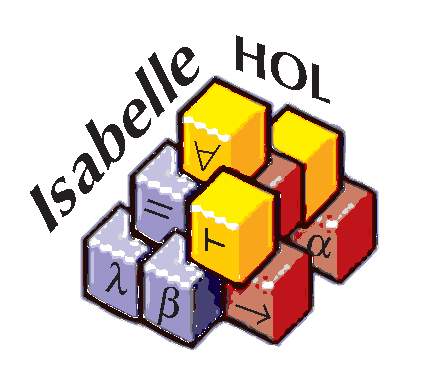
\includegraphics[scale=0.5]{isabelle_hol} \\[4ex] 
       Isabelle's Logics: HOL}

\author{Tobias Nipkow\footnote
{Institut f\"ur Informatik, Technische Universit\"at M\"unchen,
 \texttt{nipkow@in.tum.de}} and
Lawrence C. Paulson\footnote
{Computer Laboratory, University of Cambridge, \texttt{lcp@cl.cam.ac.uk}} and
Markus Wenzel\footnote
{Institut f\"ur Informatik, Technische Universit\"at M\"unchen,
 \texttt{wenzelm@in.tum.de}}}
%\thanks{The research has been funded by the EPSRC (grants
%          GR/G53279, GR/H40570, GR/K57381, GR/K77051), by ESPRIT project
%          6453: Types, and by the DFG Schwerpunktprogramm \emph{Deduktion}.}

\newcommand\subcaption[1]{\par {\centering\normalsize\sc#1\par}\bigskip
  \hrule\bigskip}
\newenvironment{constants}{\begin{center}\small\begin{tabular}{rrrr}}{\end{tabular}\end{center}}

\makeindex

\underscoreoff

\setcounter{secnumdepth}{2} \setcounter{tocdepth}{2}  %% {secnumdepth}{2}???

\pagestyle{headings}
\sloppy
\binperiod     %%%treat . like a binary operator

\begin{document}
\maketitle 

\begin{abstract}
  This manual describes Isabelle's formalization of Higher-Order Logic, a
  polymorphic version of Church's Simple Theory of Types.  HOL can be best
  understood as a simply-typed version of classical set theory.  See also
  \emph{Isabelle/HOL --- The Tutorial} for a gentle introduction on using
  Isabelle/HOL, and the \emph{Isabelle Reference Manual} for general Isabelle
  commands.
\end{abstract}

\pagenumbering{roman} \tableofcontents \clearfirst

\chapter{Syntax primitives}

The rather generic framework of Isabelle/Isar syntax emerges from three main
syntactic categories: \emph{commands} of the top-level Isar engine (covering
theory and proof elements), \emph{methods} for general goal refinements
(analogous to traditional ``tactics''), and \emph{attributes} for operations
on facts (within a certain context).  Here we give a reference of basic
syntactic entities underlying Isabelle/Isar syntax in a bottom-up manner.
Concrete theory and proof language elements will be introduced later on.

\medskip

In order to get started with writing well-formed Isabelle/Isar documents, the
most important aspect to be noted is the difference of \emph{inner} versus
\emph{outer} syntax.  Inner syntax is that of Isabelle types and terms of the
logic, while outer syntax is that of Isabelle/Isar theory sources (including
proofs).  As a general rule, inner syntax entities may occur only as
\emph{atomic entities} within outer syntax.  For example, the string
\texttt{"x + y"} and identifier \texttt{z} are legal term specifications
within a theory, while \texttt{x + y} is not.

\begin{warn}
  Old-style Isabelle theories used to fake parts of the inner syntax of types,
  with rather complicated rules when quotes may be omitted.  Despite the minor
  drawback of requiring quotes more often, the syntax of Isabelle/Isar is
  somewhat simpler and more robust in that respect.
\end{warn}

Printed theory documents usually omit quotes to gain readability (this is a
matter of {\LaTeX} macro setup, say via \verb,\isabellestyle,, see also
\cite{isabelle-sys}).  Experienced users of Isabelle/Isar may easily
reconstruct the lost technical information, while mere readers need not care
about quotes at all.

\medskip

Isabelle/Isar input may contain any number of input termination characters
``\texttt{;}'' (semicolon) to separate commands explicitly.  This is
particularly useful in interactive shell sessions to make clear where the
current command is intended to end.  Otherwise, the interpreter loop will
continue to issue a secondary prompt ``\verb,#,'' until an end-of-command is
clearly recognized from the input syntax, e.g.\ encounter of the next command
keyword.

Advanced interfaces such as Proof~General \cite{proofgeneral} do not require
explicit semicolons, the amount of input text is determined automatically by
inspecting the present content of the Emacs text buffer.  In the printed
presentation of Isabelle/Isar documents semicolons are omitted altogether for
readability.

\begin{warn}
  Proof~General requires certain syntax classification tables in order to
  achieve properly synchronized interaction with the Isabelle/Isar process.
  These tables need to be consistent with the Isabelle version and particular
  logic image to be used in a running session (common object-logics may well
  change the outer syntax).  The standard setup should work correctly with any
  of the ``official'' logic images derived from Isabelle/HOL (including HOLCF
  etc.).  Users of alternative logics may need to tell Proof~General
  explicitly, e.g.\ by giving an option \verb,-k ZF, (in conjunction with
  \verb,-l ZF, to specify the default logic image).
\end{warn}

\section{Lexical matters}\label{sec:lex-syntax}

The Isabelle/Isar outer syntax provides token classes as presented below; most
of these coincide with the inner lexical syntax as presented in
\cite{isabelle-ref}.

\indexoutertoken{ident}\indexoutertoken{longident}\indexoutertoken{symident}
\indexoutertoken{nat}\indexoutertoken{var}\indexoutertoken{typefree}
\indexoutertoken{typevar}\indexoutertoken{string}\indexoutertoken{altstring}
\indexoutertoken{verbatim}
\begin{matharray}{rcl}
  ident & = & letter\,quasiletter^* \\
  longident & = & ident (\verb,.,ident)^+ \\
  symident & = & sym^+ ~|~ \verb,\<,ident\verb,>, \\
  nat & = & digit^+ \\
  var & = & ident ~|~ \verb,?,ident ~|~ \verb,?,ident\verb,.,nat \\
  typefree & = & \verb,',ident \\
  typevar & = & typefree ~|~ \verb,?,typefree ~|~ \verb,?,typefree\verb,.,nat \\
  string & = & \verb,", ~\dots~ \verb,", \\
  altstring & = & \backquote ~\dots~ \backquote \\
  verbatim & = & \verb,{*, ~\dots~ \verb,*}, \\[1ex]

  letter & = & latin ~|~ \verb,\<,latin\verb,>, ~|~ \verb,\<,latin\,latin\verb,>, ~|~ greek ~|~ \\
         &   & \verb,\<^isub>, ~|~ \verb,\<^isup>, \\
  quasiletter & = & letter ~|~ digit ~|~ \verb,_, ~|~ \verb,', \\
  latin & = & \verb,a, ~|~ \dots ~|~ \verb,z, ~|~ \verb,A, ~|~ \dots ~|~ \verb,Z, \\
  digit & = & \verb,0, ~|~ \dots ~|~ \verb,9, \\
  sym & = & \verb,!, ~|~ \verb,#, ~|~ \verb,$, ~|~ \verb,%, ~|~ \verb,&, ~|~  %$
   \verb,*, ~|~ \verb,+, ~|~ \verb,-, ~|~ \verb,/, ~|~ \\
  & & \verb,<, ~|~ \verb,=, ~|~ \verb,>, ~|~ \verb,?, ~|~ \texttt{\at} ~|~
  \verb,^, ~|~ \verb,_, ~|~ \verb,|, ~|~ \verb,~, \\
greek & = & \verb,\<alpha>, ~|~ \verb,\<beta>, ~|~ \verb,\<gamma>, ~|~ \verb,\<delta>, ~| \\
      &   & \verb,\<epsilon>, ~|~ \verb,\<zeta>, ~|~ \verb,\<eta>, ~|~ \verb,\<theta>, ~| \\
      &   & \verb,\<iota>, ~|~ \verb,\<kappa>, ~|~ \verb,\<mu>, ~|~ \verb,\<nu>, ~| \\
      &   & \verb,\<xi>, ~|~ \verb,\<pi>, ~|~ \verb,\<rho>, ~|~ \verb,\<sigma>, ~| \\
      &   & \verb,\<tau>, ~|~ \verb,\<upsilon>, ~|~ \verb,\<phi>, ~|~ \verb,\<psi>, ~| \\
      &   & \verb,\<omega>, ~|~ \verb,\<Gamma>, ~|~ \verb,\<Delta>, ~|~ \verb,\<Theta>, ~| \\
      &   & \verb,\<Lambda>, ~|~ \verb,\<Xi>, ~|~ \verb,\<Pi>, ~|~ \verb,\<Sigma>, ~| \\
      &   & \verb,\<Upsilon>, ~|~ \verb,\<Phi>, ~|~ \verb,\<Psi>, ~|~ \verb,\<Omega>, \\
\end{matharray}

The syntax of $string$ admits any characters, including newlines; ``\verb|"|''
(double-quote) and ``\verb|\|'' (backslash) need to be escaped by a backslash.
Alternative strings according to $altstring$ are analogous, using single
back-quotes instead.  The body of $verbatim$ may consist of any text not
containing ``\verb|*}|''; this allows convenient inclusion of quotes without
further escapes.  The greek letters do \emph{not} include \verb,\<lambda>,,
which is already used differently in the meta-logic.

Common mathematical symbols such as $\forall$ are represented in Isabelle as
\verb,\<forall>,.  There are infinitely many legal symbols like this, although
proper presentation is left to front-end tools such as {\LaTeX} or
Proof~General with the X-Symbol package.  A list of standard Isabelle symbols
that work well with these tools is given in \cite[appendix~A]{isabelle-sys}.

Comments take the form \texttt{(*~\dots~*)} and may be nested, although
user-interface tools may prevent this.  Note that \texttt{(*~\dots~*)}
indicate source comments only, which are stripped after lexical analysis of
the input.  The Isar document syntax also provides formal comments that are
considered as part of the text (see \S\ref{sec:comments}).

\begin{warn}
  Proof~General does not handle nested comments properly; it is also unable to
  keep \verb,(*,\,/\,\verb,{*, and \verb,*),\,/\,\verb,*}, apart, despite
  their rather different meaning.  These are inherent problems of Emacs
  legacy.  Users should not be overly aggressive about nesting or alternating
  these delimiters.
\end{warn}


\section{Common syntax entities}

Subsequently, we introduce several basic syntactic entities, such as names,
terms, and theorem specifications, which have been factored out of the actual
Isar language elements to be described later.

Note that some of the basic syntactic entities introduced below (e.g.\
\railqtok{name}) act much like tokens rather than plain nonterminals (e.g.\
\railnonterm{sort}), especially for the sake of error messages.  E.g.\ syntax
elements like $\CONSTS$ referring to \railqtok{name} or \railqtok{type} would
really report a missing name or type rather than any of the constituent
primitive tokens such as \railtok{ident} or \railtok{string}.


\subsection{Names}

Entity \railqtok{name} usually refers to any name of types, constants,
theorems etc.\ that are to be \emph{declared} or \emph{defined} (so qualified
identifiers are excluded here).  Quoted strings provide an escape for
non-identifier names or those ruled out by outer syntax keywords (e.g.\
\verb|"let"|).  Already existing objects are usually referenced by
\railqtok{nameref}.

\indexoutertoken{name}\indexoutertoken{parname}\indexoutertoken{nameref}
\indexoutertoken{int}
\begin{rail}
  name: ident | symident | string | nat
  ;
  parname: '(' name ')'
  ;
  nameref: name | longident
  ;
  int: nat | '-' nat
  ;
\end{rail}


\subsection{Comments}\label{sec:comments}

Large chunks of plain \railqtok{text} are usually given \railtok{verbatim},
i.e.\ enclosed in \verb|{*|~\dots~\verb|*}|.  For convenience, any of the
smaller text units conforming to \railqtok{nameref} are admitted as well.  A
marginal \railnonterm{comment} is of the form \texttt{--} \railqtok{text}.
Any number of these may occur within Isabelle/Isar commands.

\indexoutertoken{text}\indexouternonterm{comment}
\begin{rail}
  text: verbatim | nameref
  ;
  comment: '--' text
  ;
\end{rail}


\subsection{Type classes, sorts and arities}

Classes are specified by plain names.  Sorts have a very simple inner syntax,
which is either a single class name $c$ or a list $\{c@1, \dots, c@n\}$
referring to the intersection of these classes.  The syntax of type arities is
given directly at the outer level.

\railalias{subseteq}{\isasymsubseteq}
\railterm{subseteq}

\indexouternonterm{sort}\indexouternonterm{arity}
\indexouternonterm{classdecl}
\begin{rail}
  classdecl: name (('<' | subseteq) (nameref + ','))?
  ;
  sort: nameref
  ;
  arity: ('(' (sort + ',') ')')? sort
  ;
\end{rail}


\subsection{Types and terms}\label{sec:types-terms}

The actual inner Isabelle syntax, that of types and terms of the logic, is far
too sophisticated in order to be modelled explicitly at the outer theory
level.  Basically, any such entity has to be quoted to turn it into a single
token (the parsing and type-checking is performed internally later).  For
convenience, a slightly more liberal convention is adopted: quotes may be
omitted for any type or term that is already atomic at the outer level.  For
example, one may just write \texttt{x} instead of \texttt{"x"}.  Note that
symbolic identifiers (e.g.\ \texttt{++} or $\forall$) are available as well,
provided these have not been superseded by commands or other keywords already
(e.g.\ \texttt{=} or \texttt{+}).

\indexoutertoken{type}\indexoutertoken{term}\indexoutertoken{prop}
\begin{rail}
  type: nameref | typefree | typevar
  ;
  term: nameref | var
  ;
  prop: term
  ;
\end{rail}

Positional instantiations are indicated by giving a sequence of terms, or the
placeholder ``$\_$'' (underscore), which means to skip a position.

\indexoutertoken{inst}\indexoutertoken{insts}
\begin{rail}
  inst: underscore | term
  ;
  insts: (inst *)
  ;
\end{rail}

Type declarations and definitions usually refer to \railnonterm{typespec} on
the left-hand side.  This models basic type constructor application at the
outer syntax level.  Note that only plain postfix notation is available here,
but no infixes.

\indexouternonterm{typespec}
\begin{rail}
  typespec: (() | typefree | '(' ( typefree + ',' ) ')') name
  ;
\end{rail}


\subsection{Mixfix annotations}

Mixfix annotations specify concrete \emph{inner} syntax of Isabelle types and
terms.  Some commands such as $\TYPES$ (see \S\ref{sec:types-pure}) admit
infixes only, while $\CONSTS$ (see \S\ref{sec:consts}) and
$\isarkeyword{syntax}$ (see \S\ref{sec:syn-trans}) support the full range of
general mixfixes and binders.

\indexouternonterm{infix}\indexouternonterm{mixfix}\indexouternonterm{structmixfix}
\begin{rail}
  infix: '(' ('infix' | 'infixl' | 'infixr') string? nat ')'
  ;
  mixfix: infix | '(' string prios? nat? ')' | '(' 'binder' string prios? nat ')'
  ;
  structmixfix: mixfix | '(' 'structure' ')'
  ;

  prios: '[' (nat + ',') ']'
  ;
\end{rail}

Here the \railtok{string} specifications refer to the actual mixfix template
(see also \cite{isabelle-ref}), which may include literal text, spacing,
blocks, and arguments (denoted by ``$_$''); the special symbol \verb,\<index>,
(printed as ``\i'') represents an index argument that specifies an implicit
structure reference (see also \S\ref{sec:locale}).  Infix and binder
declarations provide common abbreviations for particular mixfix declarations.
So in practice, mixfix templates mostly degenerate to literal text for
concrete syntax, such as ``\verb,++,'' for an infix symbol, or ``\verb,++,\i''
for an infix of an implicit structure.



\subsection{Proof methods}\label{sec:syn-meth}

Proof methods are either basic ones, or expressions composed of
methods via ``\texttt{,}'' (sequential composition), ``\texttt{|}''
(alternative choices), ``\texttt{?}'' (try), ``\texttt{+}'' (repeat at
least once), ``\texttt{[$n$]}'' (restriction to first $n$ sub-goals,
default $n = 1$).  In practice, proof methods are usually just a comma
separated list of \railqtok{nameref}~\railnonterm{args}
specifications.  Note that parentheses may be dropped for single
method specifications (with no arguments).

\indexouternonterm{method}
\begin{rail}
  method: (nameref | '(' methods ')') (() | '?' | '+' | '[' nat? ']')
  ;
  methods: (nameref args | method) + (',' | '|')
  ;
\end{rail}

Proper Isar proof methods do \emph{not} admit arbitrary goal
addressing, but refer either to the first sub-goal or all sub-goals
uniformly.  The goal restriction operator ``\texttt{[$n$]}'' evaluates
a method expression within a sandbox consisting of the first $n$
sub-goals (which need to exist).  For example,
$simp_all\mbox{\tt[}3\mbox{\tt]}$ simplifies the first three
sub-goals, while $(rule~foo, simp_all)\mbox{\tt[]}$ simplifies all new
goals that emerge from applying rule $foo$ to the originally first
one.

Improper methods, notably tactic emulations, offer a separate
low-level goal addressing scheme as explicit argument to the
individual tactic being involved.  Here $[!]$ refers to all goals, and
$[n-]$ to all goals starting from $n$,

\indexouternonterm{goalspec}
\begin{rail}
  goalspec: '[' (nat '-' nat | nat '-' | nat | '!' ) ']'
  ;
\end{rail}


\subsection{Attributes and theorems}\label{sec:syn-att}

Attributes (and proof methods, see \S\ref{sec:syn-meth}) have their own
``semi-inner'' syntax, in the sense that input conforming to
\railnonterm{args} below is parsed by the attribute a second time.  The
attribute argument specifications may be any sequence of atomic entities
(identifiers, strings etc.), or properly bracketed argument lists.  Below
\railqtok{atom} refers to any atomic entity, including any \railtok{keyword}
conforming to \railtok{symident}.

\indexoutertoken{atom}\indexouternonterm{args}\indexouternonterm{attributes}
\begin{rail}
  atom: nameref | typefree | typevar | var | nat | keyword
  ;
  arg: atom | '(' args ')' | '[' args ']'
  ;
  args: arg *
  ;
  attributes: '[' (nameref args * ',') ']'
  ;
\end{rail}

Theorem specifications come in several flavors: \railnonterm{axmdecl} and
\railnonterm{thmdecl} usually refer to axioms, assumptions or results of goal
statements, while \railnonterm{thmdef} collects lists of existing theorems.
Existing theorems are given by \railnonterm{thmref} and \railnonterm{thmrefs},
the former requires an actual singleton result.  There are three forms of
theorem references: (1) named facts $a$, (2) selections from named facts $a(i,
j - k)$, or (3) literal fact propositions using $altstring$ syntax
$\backquote\phi\backquote$, (see also method $fact$ in
\S\ref{sec:pure-meth-att}).

Any kind of theorem specification may include lists of attributes both on the
left and right hand sides; attributes are applied to any immediately preceding
fact.  If names are omitted, the theorems are not stored within the theorem
database of the theory or proof context, but any given attributes are applied
nonetheless.

\indexouternonterm{axmdecl}\indexouternonterm{thmdecl}
\indexouternonterm{thmdef}\indexouternonterm{thmref}
\indexouternonterm{thmrefs}\indexouternonterm{selection}
\begin{rail}
  axmdecl: name attributes? ':'
  ;
  thmdecl: thmbind ':'
  ;
  thmdef: thmbind '='
  ;
  thmref: (nameref selection? | altstring) attributes?
  ;
  thmrefs: thmref +
  ;

  thmbind: name attributes | name | attributes
  ;
  selection: '(' ((nat | nat '-' nat?) + ',') ')'
  ;
\end{rail}


\subsection{Term patterns and declarations}\label{sec:term-decls}

Wherever explicit propositions (or term fragments) occur in a proof text,
casual binding of schematic term variables may be given specified via patterns
of the form ``$\ISS{p@1\;\dots}{p@n}$''.  There are separate versions
available for \railqtok{term}s and \railqtok{prop}s.  The latter provides a
$\CONCLNAME$ part with patterns referring the (atomic) conclusion of a rule.

\indexouternonterm{termpat}\indexouternonterm{proppat}
\begin{rail}
  termpat: '(' ('is' term +) ')'
  ;
  proppat: '(' ('is' prop +) ')'
  ;
\end{rail}

Declarations of local variables $x :: \tau$ and logical propositions $a :
\phi$ represent different views on the same principle of introducing a local
scope.  In practice, one may usually omit the typing of $vars$ (due to
type-inference), and the naming of propositions (due to implicit references of
current facts).  In any case, Isar proof elements usually admit to introduce
multiple such items simultaneously.

\indexouternonterm{vars}\indexouternonterm{props}
\begin{rail}
  vars: (name+) ('::' type)?
  ;
  props: thmdecl? (prop proppat? +)
  ;
\end{rail}

The treatment of multiple declarations corresponds to the complementary focus
of $vars$ versus $props$: in ``$x@1~\dots~x@n :: \tau$'' the typing refers to
all variables, while in $a\colon \phi@1~\dots~\phi@n$ the naming refers to all
propositions collectively.  Isar language elements that refer to $vars$ or
$props$ typically admit separate typings or namings via another level of
iteration, with explicit $\AND$ separators; e.g.\ see $\FIXNAME$ and
$\ASSUMENAME$ in \S\ref{sec:proof-context}.


\subsection{Antiquotations}\label{sec:antiq}

\begin{matharray}{rcl}
  theory & : & \isarantiq \\
  thm & : & \isarantiq \\
  prop & : & \isarantiq \\
  term & : & \isarantiq \\
  const & : & \isarantiq \\
  abbrev & : & \isarantiq \\
  typeof & : & \isarantiq \\
  typ & : & \isarantiq \\
  thm_style & : & \isarantiq \\
  term_style & : & \isarantiq \\
  text & : & \isarantiq \\
  goals & : & \isarantiq \\
  subgoals & : & \isarantiq \\
  prf & : & \isarantiq \\
  full_prf & : & \isarantiq \\
  ML & : & \isarantiq \\
  ML_type & : & \isarantiq \\
  ML_struct & : & \isarantiq \\
\end{matharray}

The text body of formal comments (see also \S\ref{sec:comments}) may contain
antiquotations of logical entities, such as theorems, terms and types, which
are to be presented in the final output produced by the Isabelle document
preparation system (see also \S\ref{sec:document-prep}).

Thus embedding of
``\texttt{{\at}{\ttlbrace}term~[show_types]~"f(x)~=~a~+~x"{\ttrbrace}}''
within a text block would cause
\isa{(f{\isasymColon}'a~{\isasymRightarrow}~'a)~(x{\isasymColon}'a)~=~(a{\isasymColon}'a)~+~x}
to appear in the final {\LaTeX} document.  Also note that theorem
antiquotations may involve attributes as well.  For example,
\texttt{{\at}{\ttlbrace}thm~sym~[no_vars]{\ttrbrace}} would print the
statement where all schematic variables have been replaced by fixed ones,
which are easier to read.

\indexisarant{theory}\indexisarant{thm}\indexisarant{prop}\indexisarant{term}\indexisarant{const}
\indexisarant{abbrev}\indexisarant{typeof}\indexisarant{typ}\indexisarant{thm-style}
\indexisarant{term-style}\indexisarant{text}\indexisarant{goals}
\indexisarant{subgoals}\indexisarant{prf}\indexisarant{full-prf}\indexisarant{ML}
\indexisarant{ML-type}\indexisarant{ML-struct}

\begin{rail}
  atsign lbrace antiquotation rbrace
  ;

  antiquotation:
    'theory' options name |
    'thm' options thmrefs |
    'prop' options prop |
    'term' options term |
    'const' options term |
    'abbrev' options term |
    'typeof' options term |
    'typ' options type |
    'thm\_style' options name thmref |
    'term\_style' options name term |
    'text' options name |
    'goals' options |
    'subgoals' options |
    'prf' options thmrefs |
    'full\_prf' options thmrefs |
    'ML' options name |
    'ML\_type' options name |
    'ML\_struct' options name
  ;
  options: '[' (option * ',') ']'
  ;
  option: name | name '=' name
  ;
\end{rail}

Note that the syntax of antiquotations may \emph{not} include source comments
\texttt{(*~\dots~*)} or verbatim text \verb|{*|~\dots~\verb|*}|.

\begin{descr}
  
\item [$\at\{theory~A\}$] prints the name $A$, which is guaranteed to
  refer to a valid ancestor theory in the current context.

\item [$\at\{thm~\vec a\}$] prints theorems $\vec a$. Note that attribute
  specifications may be included as well (see also \S\ref{sec:syn-att}); the
  $no_vars$ operation (see \S\ref{sec:misc-meth-att}) would be particularly
  useful to suppress printing of schematic variables.

\item [$\at\{prop~\phi\}$] prints a well-typed proposition $\phi$.

\item [$\at\{term~t\}$] prints a well-typed term $t$.

\item [$\at\{const~c\}$] prints a well-defined constant $c$.
  
\item [$\at\{abbrev~c\,\vec x\}$] prints a constant abbreviation
  $c\,\vec x \equiv rhs$ as defined in the current context.

\item [$\at\{typeof~t\}$] prints the type of a well-typed term $t$.

\item [$\at\{typ~\tau\}$] prints a well-formed type $\tau$.
  
\item [$\at\{thm_style~s~a\}$] prints theorem $a$, previously applying a style
  $s$ to it (see below).
  
\item [$\at\{term_style~s~t\}$] prints a well-typed term $t$ after applying a
  style $s$ to it (see below).

\item [$\at\{text~s\}$] prints uninterpreted source text $s$.  This is
  particularly useful to print portions of text according to the Isabelle
  {\LaTeX} output style, without demanding well-formedness (e.g.\ small pieces
  of terms that should not be parsed or type-checked yet).

\item [$\at\{goals\}$] prints the current \emph{dynamic} goal state.  This is
  mainly for support of tactic-emulation scripts within Isar --- presentation
  of goal states does not conform to actual human-readable proof documents.
  Please do not include goal states into document output unless you really
  know what you are doing!
  
\item [$\at\{subgoals\}$] is similar to $goals$, but does not print the main
  goal.
  
\item [$\at\{prf~\vec a\}$] prints the (compact) proof terms corresponding to
  the theorems $\vec a$. Note that this requires proof terms to be switched on
  for the current object logic (see the ``Proof terms'' section of the
  Isabelle reference manual for information on how to do this).
  
\item [$\at\{full_prf~\vec a\}$] is like $\at\{prf~\vec a\}$, but displays the
  full proof terms, i.e.\ also displays information omitted in the compact
  proof term, which is denoted by ``$_$'' placeholders there.
  
\item [$\at\{ML~s\}$, $\at\{ML_type~s\}$, and $\at\{ML_struct~s\}$] check text
  $s$ as ML value, type, and structure, respectively.  If successful, the
  source is displayed verbatim.

\end{descr}

\medskip

The following standard styles for use with $thm_style$ and $term_style$ are
available:

\begin{descr}
  
\item [$lhs$] extracts the first argument of any application form with at
  least two arguments -- typically meta-level or object-level equality, or any
  other binary relation.
  
\item [$rhs$] is like $lhs$, but extracts the second argument.
  
\item [$concl$] extracts the conclusion $C$ from a nested meta-level
  implication $A@1 \Imp \cdots A@n \Imp C$.
  
\item [$prem1$, \dots, $prem9$] extract premise number $1$, \dots, $9$,
  respectively, from a nested meta-level implication $A@1 \Imp \cdots A@n \Imp
  C$.

\end{descr}

\medskip

The following options are available to tune the output.  Note that most of
these coincide with ML flags of the same names (see also \cite{isabelle-ref}).
\begin{descr}
\item[$show_types = bool$ and $show_sorts = bool$] control printing of
  explicit type and sort constraints.
\item[$show_structs = bool$] controls printing of implicit structures.
\item[$long_names = bool$] forces names of types and constants etc.\ to be
  printed in their fully qualified internal form.
\item[$short_names = bool$] forces names of types and constants etc.\ to be
  printed unqualified.  Note that internalizing the output again in the
  current context may well yield a different result.
\item[$unique_names = bool$] determines whether the printed version of
  qualified names should be made sufficiently long to avoid overlap with names
  declared further back.  Set to $false$ for more concise output.
\item[$eta_contract = bool$] prints terms in $\eta$-contracted form.
\item[$display = bool$] indicates if the text is to be output as multi-line
  ``display material'', rather than a small piece of text without line breaks
  (which is the default).
\item[$breaks = bool$] controls line breaks in non-display material.
\item[$quotes = bool$] indicates if the output should be enclosed in double
  quotes.
\item[$mode = name$] adds $name$ to the print mode to be used for presentation
  (see also \cite{isabelle-ref}).  Note that the standard setup for {\LaTeX}
  output is already present by default, including the modes ``$latex$'',
  ``$xsymbols$'', ``$symbols$''.
\item[$margin = nat$ and $indent = nat$] change the margin or indentation for
  pretty printing of display material.
\item[$source = bool$] prints the source text of the antiquotation arguments,
  rather than the actual value.  Note that this does not affect
  well-formedness checks of $thm$, $term$, etc. (only the $text$ antiquotation
  admits arbitrary output).
\item[$goals_limit = nat$] determines the maximum number of goals to be
  printed.
\item[$locale = name$] specifies an alternative context used for evaluating
  and printing the subsequent argument.
\end{descr}

For boolean flags, ``$name = true$'' may be abbreviated as ``$name$''.  All of
the above flags are disabled by default, unless changed from ML.

\medskip Note that antiquotations do not only spare the author from tedious
typing of logical entities, but also achieve some degree of
consistency-checking of informal explanations with formal developments:
well-formedness of terms and types with respect to the current theory or proof
context is ensured here.


\subsection{Tagged commands}\label{sec:tags}

Each Isabelle/Isar command may be decorated by presentation tags:

\indexouternonterm{tags}
\begin{rail}
  tags: ( tag * )
  ;
  tag: '\%' (ident | string)
\end{rail}

The tags $theory$, $proof$, $ML$ are already pre-declared for certain classes
of commands:

\medskip

\begin{tabular}{ll}
  $theory$ & theory begin and end \\
  $proof$ & all proof commands \\
  $ML$ & all commands involving ML code \\
\end{tabular}

\medskip The Isabelle document preparation system (see also
\cite{isabelle-sys}) allows tagged command regions to be presented
specifically, e.g.\ to fold proof texts, or drop parts of the text completely.

For example ``$\BYNAME~\%invisible~(auto)$'' would cause that piece of proof
to be treated as $invisible$ instead of $proof$ (the default), which may be
either show or hidden depending on the document setup.  In contrast,
``$\BYNAME~\%visible~(auto)$'' would force this text to be shown invariably.

Explicit tag specifications within a proof apply to all subsequent commands of
the same level of nesting.  For example,
``$\PROOFNAME~\%visible~\dots\QEDNAME$'' would force the whole sub-proof to be
typeset as $visible$ (unless some of its parts are tagged differently).

%%% Local Variables:
%%% mode: latex
%%% TeX-master: "isar-ref"
%%% End:

%% $Id$
\chapter{Higher-Order Logic}
\index{higher-order logic|(}
\index{HOL system@{\sc hol} system}

The theory~\thydx{HOL} implements higher-order logic.  It is based on
Gordon's~{\sc hol} system~\cite{mgordon-hol}, which itself is based on
Church's original paper~\cite{church40}.  Andrews's
book~\cite{andrews86} is a full description of the original
Church-style higher-order logic.  Experience with the {\sc hol} system
has demonstrated that higher-order logic is widely applicable in many
areas of mathematics and computer science, not just hardware
verification, {\sc hol}'s original {\it raison d'\^etre\/}.  It is
weaker than {\ZF} set theory but for most applications this does not
matter.  If you prefer {\ML} to Lisp, you will probably prefer \HOL\ 
to~{\ZF}.

The syntax of \HOL\footnote{Earlier versions of Isabelle's \HOL\ used a
different syntax. Ancient releases of Isabelle included still another version
of~\HOL, with explicit type inference rules~\cite{paulson-COLOG}.  This
version no longer exists, but \thydx{ZF} supports a similar style of
reasoning.} follows $\lambda$-calculus and functional programming.  Function
application is curried.  To apply the function~$f$ of type
$\tau@1\To\tau@2\To\tau@3$ to the arguments~$a$ and~$b$ in \HOL, you simply
write $f\,a\,b$. There is no `apply' operator as in \thydx{ZF}. Note that
$f(a,b)$ means ``$f$ applied to the pair $(a,b)$'' in \HOL.  We write ordered
pairs as $(a,b)$, not $\langle a,b\rangle$ as in {\ZF}.

\HOL\ has a distinct feel, compared with {\ZF} and {\CTT}.  It
identifies object-level types with meta-level types, taking advantage of
Isabelle's built-in type checker.  It identifies object-level functions
with meta-level functions, so it uses Isabelle's operations for abstraction
and application.

These identifications allow Isabelle to support \HOL\ particularly
nicely, but they also mean that \HOL\ requires more sophistication
from the user --- in particular, an understanding of Isabelle's type
system.  Beginners should work with {\tt show_types} (or even
\texttt{show_sorts}) set to {\tt true}.
%  Gain experience by
%working in first-order logic before attempting to use higher-order logic.
%This chapter assumes familiarity with~{\FOL{}}.


\begin{figure}
\begin{constants}
  \it name      &\it meta-type  & \it description \\
  \cdx{Trueprop}& $bool\To prop$                & coercion to $prop$\\
  \cdx{Not}     & $bool\To bool$                & negation ($\neg$) \\
  \cdx{True}    & $bool$                        & tautology ($\top$) \\
  \cdx{False}   & $bool$                        & absurdity ($\bot$) \\
  \cdx{If}      & $[bool,\alpha,\alpha]\To\alpha$ & conditional \\
  \cdx{Let}     & $[\alpha,\alpha\To\beta]\To\beta$ & let binder
\end{constants}
\subcaption{Constants}

\begin{constants}
\index{"@@{\tt\at} symbol}
\index{*"! symbol}\index{*"? symbol}
\index{*"?"! symbol}\index{*"E"X"! symbol}
  \it symbol &\it name     &\it meta-type & \it description \\
  \tt\at & \cdx{Eps}  & $(\alpha\To bool)\To\alpha$ & 
        Hilbert description ($\varepsilon$) \\
  {\tt!~} or \sdx{ALL}  & \cdx{All}  & $(\alpha\To bool)\To bool$ & 
        universal quantifier ($\forall$) \\
  {\tt?~} or \sdx{EX}   & \cdx{Ex}   & $(\alpha\To bool)\To bool$ & 
        existential quantifier ($\exists$) \\
  {\tt?!} or {\tt EX!}  & \cdx{Ex1}  & $(\alpha\To bool)\To bool$ & 
        unique existence ($\exists!$)\\
  {\tt LEAST}  & \cdx{Least}  & $(\alpha::ord \To bool)\To\alpha$ & 
        least element
\end{constants}
\subcaption{Binders} 

\begin{constants}
\index{*"= symbol}
\index{&@{\tt\&} symbol}
\index{*"| symbol}
\index{*"-"-"> symbol}
  \it symbol    & \it meta-type & \it priority & \it description \\ 
  \sdx{o}       & $[\beta\To\gamma,\alpha\To\beta]\To (\alpha\To\gamma)$ & 
        Left 55 & composition ($\circ$) \\
  \tt =         & $[\alpha,\alpha]\To bool$ & Left 50 & equality ($=$) \\
  \tt <         & $[\alpha::ord,\alpha]\To bool$ & Left 50 & less than ($<$) \\
  \tt <=        & $[\alpha::ord,\alpha]\To bool$ & Left 50 & 
                less than or equals ($\leq$)\\
  \tt \&        & $[bool,bool]\To bool$ & Right 35 & conjunction ($\conj$) \\
  \tt |         & $[bool,bool]\To bool$ & Right 30 & disjunction ($\disj$) \\
  \tt -->       & $[bool,bool]\To bool$ & Right 25 & implication ($\imp$)
\end{constants}
\subcaption{Infixes}
\caption{Syntax of {\tt HOL}} \label{hol-constants}
\end{figure}


\begin{figure}
\index{*let symbol}
\index{*in symbol}
\dquotes
\[\begin{array}{rclcl}
    term & = & \hbox{expression of class~$term$} \\
         & | & "\at~" id " . " formula \\
         & | & 
    \multicolumn{3}{l}{"let"~id~"="~term";"\dots";"~id~"="~term~"in"~term} \\
         & | & 
    \multicolumn{3}{l}{"if"~formula~"then"~term~"else"~term} \\
         & | & "LEAST"~ id " . " formula \\[2ex]
 formula & = & \hbox{expression of type~$bool$} \\
         & | & term " = " term \\
         & | & term " \ttilde= " term \\
         & | & term " < " term \\
         & | & term " <= " term \\
         & | & "\ttilde\ " formula \\
         & | & formula " \& " formula \\
         & | & formula " | " formula \\
         & | & formula " --> " formula \\
         & | & "!~~~" id~id^* " . " formula 
         & | & "ALL~" id~id^* " . " formula \\
         & | & "?~~~" id~id^* " . " formula 
         & | & "EX~~" id~id^* " . " formula \\
         & | & "?!~~" id~id^* " . " formula 
         & | & "EX!~" id~id^* " . " formula
  \end{array}
\]
\caption{Full grammar for \HOL} \label{hol-grammar}
\end{figure} 


\section{Syntax}

Figure~\ref{hol-constants} lists the constants (including infixes and
binders), while Fig.\ts\ref{hol-grammar} presents the grammar of
higher-order logic.  Note that $a$\verb|~=|$b$ is translated to
$\neg(a=b)$.

\begin{warn}
  \HOL\ has no if-and-only-if connective; logical equivalence is expressed
  using equality.  But equality has a high priority, as befitting a
  relation, while if-and-only-if typically has the lowest priority.  Thus,
  $\neg\neg P=P$ abbreviates $\neg\neg (P=P)$ and not $(\neg\neg P)=P$.
  When using $=$ to mean logical equivalence, enclose both operands in
  parentheses.
\end{warn}

\subsection{Types and classes}
The universal type class of higher-order terms is called~\cldx{term}.
By default, explicit type variables have class \cldx{term}.  In
particular the equality symbol and quantifiers are polymorphic over
class {\tt term}.

The type of formulae, \tydx{bool}, belongs to class \cldx{term}; thus,
formulae are terms.  The built-in type~\tydx{fun}, which constructs
function types, is overloaded with arity {\tt(term,\thinspace
  term)\thinspace term}.  Thus, $\sigma\To\tau$ belongs to class~{\tt
  term} if $\sigma$ and~$\tau$ do, allowing quantification over
functions.

\HOL\ offers various methods for introducing new types.
See~\S\ref{sec:HOL:Types} and~\S\ref{sec:HOL:datatype}.

Theory \thydx{Ord} defines the syntactic class \cldx{ord} of order
signatures; the relations $<$ and $\leq$ are polymorphic over this
class, as are the functions \cdx{mono}, \cdx{min} and \cdx{max}, and
the \cdx{LEAST} operator. \thydx{Ord} also defines a subclass
\cldx{order} of \cldx{ord} which axiomatizes partially ordered types
(w.r.t.\ $\le$).

Three other syntactic type classes --- \cldx{plus}, \cldx{minus} and
\cldx{times} --- permit overloading of the operators {\tt+},\index{*"+
  symbol} {\tt-}\index{*"- symbol} and {\tt*}.\index{*"* symbol} In
particular, {\tt-} is instantiated for set difference and subtraction
on natural numbers.

If you state a goal containing overloaded functions, you may need to include
type constraints.  Type inference may otherwise make the goal more
polymorphic than you intended, with confusing results. For example, the
variables $i$, $j$ and $k$ in the goal $i \le j \Imp i \le j+k$ have type
$\alpha::\{ord,plus\}$, although you may have expected them to have some
numeric type, e.g. $nat$. Instead you should have stated the goal as
$(i::nat) \le j \Imp i \le j+k$, which causes all three variables to have
type $nat$.

\begin{warn}
  If resolution fails for no obvious reason, try setting
  \ttindex{show_types} to {\tt true}, causing Isabelle to display
  types of terms.  Possibly set \ttindex{show_sorts} to {\tt true} as
  well, causing Isabelle to display type classes and sorts.

  \index{unification!incompleteness of}
  Where function types are involved, Isabelle's unification code does not
  guarantee to find instantiations for type variables automatically.  Be
  prepared to use \ttindex{res_inst_tac} instead of {\tt resolve_tac},
  possibly instantiating type variables.  Setting
  \ttindex{Unify.trace_types} to {\tt true} causes Isabelle to report
  omitted search paths during unification.\index{tracing!of unification}
\end{warn}


\subsection{Binders}

Hilbert's {\bf description} operator~$\varepsilon x.P[x]$ stands for
some~$x$ satisfying~$P$, if such exists.  Since all terms in \HOL\ 
denote something, a description is always meaningful, but we do not
know its value unless $P$ defines it uniquely.  We may write
descriptions as \cdx{Eps}($\lambda x.P[x]$) or use the syntax
\hbox{\tt \at $x$.$P[x]$}.

Existential quantification is defined by
\[ \exists x.P~x \;\equiv\; P(\varepsilon x.P~x). \]
The unique existence quantifier, $\exists!x.P$, is defined in terms
of~$\exists$ and~$\forall$.  An Isabelle binder, it admits nested
quantifications.  For instance, $\exists!x\,y.P\,x\,y$ abbreviates
$\exists!x. \exists!y.P\,x\,y$; note that this does not mean that there
exists a unique pair $(x,y)$ satisfying~$P\,x\,y$.

\index{*"! symbol}\index{*"? symbol}\index{HOL system@{\sc hol} system}
Quantifiers have two notations.  As in Gordon's {\sc hol} system, \HOL\
uses~{\tt!}\ and~{\tt?}\ to stand for $\forall$ and $\exists$.  The
existential quantifier must be followed by a space; thus {\tt?x} is an
unknown, while \verb'? x.f x=y' is a quantification.  Isabelle's usual
notation for quantifiers, \sdx{ALL} and \sdx{EX}, is also
available.  Both notations are accepted for input.  The {\ML} reference
\ttindexbold{HOL_quantifiers} governs the output notation.  If set to {\tt
true}, then~{\tt!}\ and~{\tt?}\ are displayed; this is the default.  If set
to {\tt false}, then~{\tt ALL} and~{\tt EX} are displayed.

If $\tau$ is a type of class \cldx{ord}, $P$ a formula and $x$ a
variable of type $\tau$, then the term \cdx{LEAST}~$x.P[x]$ is defined
to be the least (w.r.t.\ $\le$) $x$ such that $P~x$ holds (see
Fig.~\ref{hol-defs}). The definition uses Hilbert's $\varepsilon$
choice operator, so \texttt{Least} is always meaningful, but may yield
nothing useful in case there is not a unique least element satisfying
$P$.\footnote{Class $ord$ does not require much of its instances, so
  $\le$ need not be a well-ordering, not even an order at all!}

\medskip All these binders have priority 10.

\begin{warn}
The low priority of binders means that they need to be enclosed in
parenthesis when they occur in the context of other operations. For example,
instead of $P \land \forall x.Q$ you need to write $P \land (\forall x.Q)$.
\end{warn}


\subsection{The \sdx{let} and \sdx{case} constructions}
Local abbreviations can be introduced by a {\tt let} construct whose
syntax appears in Fig.\ts\ref{hol-grammar}.  Internally it is translated into
the constant~\cdx{Let}.  It can be expanded by rewriting with its
definition, \tdx{Let_def}.

\HOL\ also defines the basic syntax
\[\dquotes"case"~e~"of"~c@1~"=>"~e@1~"|" \dots "|"~c@n~"=>"~e@n\] 
as a uniform means of expressing {\tt case} constructs.  Therefore {\tt case}
and \sdx{of} are reserved words.  Initially, this is mere syntax and has no
logical meaning.  By declaring translations, you can cause instances of the
{\tt case} construct to denote applications of particular case operators.
This is what happens automatically for each {\tt datatype} definition
(see~\S\ref{sec:HOL:datatype}).

\begin{warn}
Both {\tt if} and {\tt case} constructs have as low a priority as
quantifiers, which requires additional enclosing parentheses in the context
of most other operations. For example, instead of $f~x = if \dots then \dots
else \dots$ you need to write $f~x = (if \dots then \dots else
\dots)$.
\end{warn}

\section{Rules of inference}

\begin{figure}
\begin{ttbox}\makeatother
\tdx{refl}           t = (t::'a)
\tdx{subst}          [| s = t; P s |] ==> P (t::'a)
\tdx{ext}            (!!x::'a. (f x :: 'b) = g x) ==> (\%x.f x) = (\%x.g x)
\tdx{impI}           (P ==> Q) ==> P-->Q
\tdx{mp}             [| P-->Q;  P |] ==> Q
\tdx{iff}            (P-->Q) --> (Q-->P) --> (P=Q)
\tdx{selectI}        P(x::'a) ==> P(@x.P x)
\tdx{True_or_False}  (P=True) | (P=False)
\end{ttbox}
\caption{The {\tt HOL} rules} \label{hol-rules}
\end{figure}

Figure~\ref{hol-rules} shows the primitive inference rules of~\HOL{},
with their~{\ML} names.  Some of the rules deserve additional
comments:
\begin{ttdescription}
\item[\tdx{ext}] expresses extensionality of functions.
\item[\tdx{iff}] asserts that logically equivalent formulae are
  equal.
\item[\tdx{selectI}] gives the defining property of the Hilbert
  $\varepsilon$-operator.  It is a form of the Axiom of Choice.  The derived rule
  \tdx{select_equality} (see below) is often easier to use.
\item[\tdx{True_or_False}] makes the logic classical.\footnote{In
    fact, the $\varepsilon$-operator already makes the logic classical, as
    shown by Diaconescu; see Paulson~\cite{paulson-COLOG} for details.}
\end{ttdescription}


\begin{figure}\hfuzz=4pt%suppress "Overfull \hbox" message
\begin{ttbox}\makeatother
\tdx{True_def}   True     == ((\%x::bool.x)=(\%x.x))
\tdx{All_def}    All      == (\%P. P = (\%x.True))
\tdx{Ex_def}     Ex       == (\%P. P(@x.P x))
\tdx{False_def}  False    == (!P.P)
\tdx{not_def}    not      == (\%P. P-->False)
\tdx{and_def}    op &     == (\%P Q. !R. (P-->Q-->R) --> R)
\tdx{or_def}     op |     == (\%P Q. !R. (P-->R) --> (Q-->R) --> R)
\tdx{Ex1_def}    Ex1      == (\%P. ? x. P x & (! y. P y --> y=x))

\tdx{o_def}      op o     == (\%(f::'b=>'c) g x::'a. f(g x))
\tdx{if_def}     If P x y ==
              (\%P x y. @z::'a.(P=True --> z=x) & (P=False --> z=y))
\tdx{Let_def}    Let s f  == f s
\tdx{Least_def}  Least P  == @x. P(x) & (ALL y. P(y) --> x <= y)"
\end{ttbox}
\caption{The {\tt HOL} definitions} \label{hol-defs}
\end{figure}


\HOL{} follows standard practice in higher-order logic: only a few
connectives are taken as primitive, with the remainder defined obscurely
(Fig.\ts\ref{hol-defs}).  Gordon's {\sc hol} system expresses the
corresponding definitions \cite[page~270]{mgordon-hol} using
object-equality~({\tt=}), which is possible because equality in
higher-order logic may equate formulae and even functions over formulae.
But theory~\HOL{}, like all other Isabelle theories, uses
meta-equality~({\tt==}) for definitions.
\begin{warn}
The definitions above should never be expanded and are shown for completeness
only. Instead users should reason in terms of the derived rules shown below
or, better still, using high-level tactics
(see~\S\ref{sec:HOL:generic-packages}).
\end{warn}

Some of the rules mention type variables; for example, {\tt refl}
mentions the type variable~{\tt'a}.  This allows you to instantiate
type variables explicitly by calling {\tt res_inst_tac}.


\begin{figure}
\begin{ttbox}
\tdx{sym}         s=t ==> t=s
\tdx{trans}       [| r=s; s=t |] ==> r=t
\tdx{ssubst}      [| t=s; P s |] ==> P t
\tdx{box_equals}  [| a=b;  a=c;  b=d |] ==> c=d  
\tdx{arg_cong}    x = y ==> f x = f y
\tdx{fun_cong}    f = g ==> f x = g x
\tdx{cong}        [| f = g; x = y |] ==> f x = g y
\tdx{not_sym}     t ~= s ==> s ~= t
\subcaption{Equality}

\tdx{TrueI}       True 
\tdx{FalseE}      False ==> P

\tdx{conjI}       [| P; Q |] ==> P&Q
\tdx{conjunct1}   [| P&Q |] ==> P
\tdx{conjunct2}   [| P&Q |] ==> Q 
\tdx{conjE}       [| P&Q;  [| P; Q |] ==> R |] ==> R

\tdx{disjI1}      P ==> P|Q
\tdx{disjI2}      Q ==> P|Q
\tdx{disjE}       [| P | Q; P ==> R; Q ==> R |] ==> R

\tdx{notI}        (P ==> False) ==> ~ P
\tdx{notE}        [| ~ P;  P |] ==> R
\tdx{impE}        [| P-->Q;  P;  Q ==> R |] ==> R
\subcaption{Propositional logic}

\tdx{iffI}        [| P ==> Q;  Q ==> P |] ==> P=Q
\tdx{iffD1}       [| P=Q; P |] ==> Q
\tdx{iffD2}       [| P=Q; Q |] ==> P
\tdx{iffE}        [| P=Q; [| P --> Q; Q --> P |] ==> R |] ==> R
%
%\tdx{eqTrueI}     P ==> P=True 
%\tdx{eqTrueE}     P=True ==> P 
\subcaption{Logical equivalence}

\end{ttbox}
\caption{Derived rules for \HOL} \label{hol-lemmas1}
\end{figure}


\begin{figure}
\begin{ttbox}\makeatother
\tdx{allI}      (!!x. P x) ==> !x. P x
\tdx{spec}      !x.P x ==> P x
\tdx{allE}      [| !x.P x;  P x ==> R |] ==> R
\tdx{all_dupE}  [| !x.P x;  [| P x; !x.P x |] ==> R |] ==> R

\tdx{exI}       P x ==> ? x. P x
\tdx{exE}       [| ? x. P x; !!x. P x ==> Q |] ==> Q

\tdx{ex1I}      [| P a;  !!x. P x ==> x=a |] ==> ?! x. P x
\tdx{ex1E}      [| ?! x.P x;  !!x. [| P x;  ! y. P y --> y=x |] ==> R 
          |] ==> R

\tdx{select_equality} [| P a;  !!x. P x ==> x=a |] ==> (@x.P x) = a
\subcaption{Quantifiers and descriptions}

\tdx{ccontr}          (~P ==> False) ==> P
\tdx{classical}       (~P ==> P) ==> P
\tdx{excluded_middle} ~P | P

\tdx{disjCI}          (~Q ==> P) ==> P|Q
\tdx{exCI}            (! x. ~ P x ==> P a) ==> ? x.P x
\tdx{impCE}           [| P-->Q; ~ P ==> R; Q ==> R |] ==> R
\tdx{iffCE}           [| P=Q;  [| P;Q |] ==> R;  [| ~P; ~Q |] ==> R |] ==> R
\tdx{notnotD}         ~~P ==> P
\tdx{swap}            ~P ==> (~Q ==> P) ==> Q
\subcaption{Classical logic}

%\tdx{if_True}         (if True then x else y) = x
%\tdx{if_False}        (if False then x else y) = y
\tdx{if_P}            P ==> (if P then x else y) = x
\tdx{if_not_P}        ~ P ==> (if P then x else y) = y
\tdx{expand_if}       P(if Q then x else y) = ((Q --> P x) & (~Q --> P y))
\subcaption{Conditionals}
\end{ttbox}
\caption{More derived rules} \label{hol-lemmas2}
\end{figure}

Some derived rules are shown in Figures~\ref{hol-lemmas1}
and~\ref{hol-lemmas2}, with their {\ML} names.  These include natural rules
for the logical connectives, as well as sequent-style elimination rules for
conjunctions, implications, and universal quantifiers.  

Note the equality rules: \tdx{ssubst} performs substitution in
backward proofs, while \tdx{box_equals} supports reasoning by
simplifying both sides of an equation.

The following simple tactics are occasionally useful:
\begin{ttdescription}
\item[\ttindexbold{strip_tac} $i$] applies {\tt allI} and {\tt impI}
  repeatedly to remove all outermost universal quantifiers and implications
  from subgoal $i$.
\item[\ttindexbold{case_tac} {\tt"}$P${\tt"} $i$] performs case distinction
  on $P$ for subgoal $i$: the latter is replaced by two identical subgoals
  with the added assumptions $P$ and $\neg P$, respectively.
\end{ttdescription}


\begin{figure} 
\begin{center}
\begin{tabular}{rrr}
  \it name      &\it meta-type  & \it description \\ 
\index{{}@\verb'{}' symbol}
  \verb|{}|     & $\alpha\,set$         & the empty set \\
  \cdx{insert}  & $[\alpha,\alpha\,set]\To \alpha\,set$
        & insertion of element \\
  \cdx{Collect} & $(\alpha\To bool)\To\alpha\,set$
        & comprehension \\
  \cdx{Compl}   & $\alpha\,set\To\alpha\,set$
        & complement \\
  \cdx{INTER} & $[\alpha\,set,\alpha\To\beta\,set]\To\beta\,set$
        & intersection over a set\\
  \cdx{UNION} & $[\alpha\,set,\alpha\To\beta\,set]\To\beta\,set$
        & union over a set\\
  \cdx{Inter} & $(\alpha\,set)set\To\alpha\,set$
        &set of sets intersection \\
  \cdx{Union} & $(\alpha\,set)set\To\alpha\,set$
        &set of sets union \\
  \cdx{Pow}   & $\alpha\,set \To (\alpha\,set)set$
        & powerset \\[1ex]
  \cdx{range}   & $(\alpha\To\beta )\To\beta\,set$
        & range of a function \\[1ex]
  \cdx{Ball}~~\cdx{Bex} & $[\alpha\,set,\alpha\To bool]\To bool$
        & bounded quantifiers
\end{tabular}
\end{center}
\subcaption{Constants}

\begin{center}
\begin{tabular}{llrrr} 
  \it symbol &\it name     &\it meta-type & \it priority & \it description \\
  \sdx{INT}  & \cdx{INTER1}  & $(\alpha\To\beta\,set)\To\beta\,set$ & 10 & 
        intersection over a type\\
  \sdx{UN}  & \cdx{UNION1}  & $(\alpha\To\beta\,set)\To\beta\,set$ & 10 & 
        union over a type
\end{tabular}
\end{center}
\subcaption{Binders} 

\begin{center}
\index{*"`"` symbol}
\index{*": symbol}
\index{*"<"= symbol}
\begin{tabular}{rrrr} 
  \it symbol    & \it meta-type & \it priority & \it description \\ 
  \tt ``        & $[\alpha\To\beta ,\alpha\,set]\To  \beta\,set$
        & Left 90 & image \\
  \sdx{Int}     & $[\alpha\,set,\alpha\,set]\To\alpha\,set$
        & Left 70 & intersection ($\int$) \\
  \sdx{Un}      & $[\alpha\,set,\alpha\,set]\To\alpha\,set$
        & Left 65 & union ($\un$) \\
  \tt:          & $[\alpha ,\alpha\,set]\To bool$       
        & Left 50 & membership ($\in$) \\
  \tt <=        & $[\alpha\,set,\alpha\,set]\To bool$
        & Left 50 & subset ($\subseteq$) 
\end{tabular}
\end{center}
\subcaption{Infixes}
\caption{Syntax of the theory {\tt Set}} \label{hol-set-syntax}
\end{figure} 


\begin{figure} 
\begin{center} \tt\frenchspacing
\index{*"! symbol}
\begin{tabular}{rrr} 
  \it external          & \it internal  & \it description \\ 
  $a$ \ttilde: $b$      & \ttilde($a$ : $b$)    & \rm non-membership\\
  {\ttlbrace}$a@1$, $\ldots${\ttrbrace}  &  insert $a@1$ $\ldots$ {\ttlbrace}{\ttrbrace} & \rm finite set \\
  {\ttlbrace}$x$.$P[x]${\ttrbrace}        &  Collect($\lambda x.P[x]$) &
        \rm comprehension \\
  \sdx{INT} $x$:$A$.$B[x]$      & INTER $A$ $\lambda x.B[x]$ &
        \rm intersection \\
  \sdx{UN}{\tt\ }  $x$:$A$.$B[x]$      & UNION $A$ $\lambda x.B[x]$ &
        \rm union \\
  \tt ! $x$:$A$.$P[x]$ or \sdx{ALL} $x$:$A$.$P[x]$ & 
        Ball $A$ $\lambda x.P[x]$ & 
        \rm bounded $\forall$ \\
  \sdx{?} $x$:$A$.$P[x]$ or \sdx{EX}{\tt\ } $x$:$A$.$P[x]$ & 
        Bex $A$ $\lambda x.P[x]$ & \rm bounded $\exists$
\end{tabular}
\end{center}
\subcaption{Translations}

\dquotes
\[\begin{array}{rclcl}
    term & = & \hbox{other terms\ldots} \\
         & | & "{\ttlbrace}{\ttrbrace}" \\
         & | & "{\ttlbrace} " term\; ("," term)^* " {\ttrbrace}" \\
         & | & "{\ttlbrace} " id " . " formula " {\ttrbrace}" \\
         & | & term " `` " term \\
         & | & term " Int " term \\
         & | & term " Un " term \\
         & | & "INT~~"  id ":" term " . " term \\
         & | & "UN~~~"  id ":" term " . " term \\
         & | & "INT~~"  id~id^* " . " term \\
         & | & "UN~~~"  id~id^* " . " term \\[2ex]
 formula & = & \hbox{other formulae\ldots} \\
         & | & term " : " term \\
         & | & term " \ttilde: " term \\
         & | & term " <= " term \\
         & | & "!~" id ":" term " . " formula 
         & | & "ALL " id ":" term " . " formula \\
         & | & "?~" id ":" term " . " formula 
         & | & "EX~~" id ":" term " . " formula
  \end{array}
\]
\subcaption{Full Grammar}
\caption{Syntax of the theory {\tt Set} (continued)} \label{hol-set-syntax2}
\end{figure} 


\section{A formulation of set theory}
Historically, higher-order logic gives a foundation for Russell and
Whitehead's theory of classes.  Let us use modern terminology and call them
{\bf sets}, but note that these sets are distinct from those of {\ZF} set
theory, and behave more like {\ZF} classes.
\begin{itemize}
\item
Sets are given by predicates over some type~$\sigma$.  Types serve to
define universes for sets, but type checking is still significant.
\item
There is a universal set (for each type).  Thus, sets have complements, and
may be defined by absolute comprehension.
\item
Although sets may contain other sets as elements, the containing set must
have a more complex type.
\end{itemize}
Finite unions and intersections have the same behaviour in \HOL\ as they
do in~{\ZF}.  In \HOL\ the intersection of the empty set is well-defined,
denoting the universal set for the given type.

\subsection{Syntax of set theory}\index{*set type}
\HOL's set theory is called \thydx{Set}.  The type $\alpha\,set$ is
essentially the same as $\alpha\To bool$.  The new type is defined for
clarity and to avoid complications involving function types in unification.
The isomorphisms between the two types are declared explicitly.  They are
very natural: {\tt Collect} maps $\alpha\To bool$ to $\alpha\,set$, while
\hbox{\tt op :} maps in the other direction (ignoring argument order).

Figure~\ref{hol-set-syntax} lists the constants, infixes, and syntax
translations.  Figure~\ref{hol-set-syntax2} presents the grammar of the new
constructs.  Infix operators include union and intersection ($A\un B$
and $A\int B$), the subset and membership relations, and the image
operator~{\tt``}\@.  Note that $a$\verb|~:|$b$ is translated to
$\neg(a\in b)$.  

The $\{a@1,\ldots\}$ notation abbreviates finite sets constructed in
the obvious manner using~{\tt insert} and~$\{\}$:
\begin{eqnarray*}
  \{a, b, c\} & \equiv &
  {\tt insert} \, a \, ({\tt insert} \, b \, ({\tt insert} \, c \, \{\}))
\end{eqnarray*}

The set \hbox{\tt{\ttlbrace}$x$.$P[x]${\ttrbrace}} consists of all $x$ (of suitable type)
that satisfy~$P[x]$, where $P[x]$ is a formula that may contain free
occurrences of~$x$.  This syntax expands to \cdx{Collect}$(\lambda
x.P[x])$.  It defines sets by absolute comprehension, which is impossible
in~{\ZF}; the type of~$x$ implicitly restricts the comprehension.

The set theory defines two {\bf bounded quantifiers}:
\begin{eqnarray*}
   \forall x\in A.P[x] &\hbox{abbreviates}& \forall x. x\in A\imp P[x] \\
   \exists x\in A.P[x] &\hbox{abbreviates}& \exists x. x\in A\conj P[x]
\end{eqnarray*}
The constants~\cdx{Ball} and~\cdx{Bex} are defined
accordingly.  Instead of {\tt Ball $A$ $P$} and {\tt Bex $A$ $P$} we may
write\index{*"! symbol}\index{*"? symbol}
\index{*ALL symbol}\index{*EX symbol} 
%
\hbox{\tt !~$x$:$A$.$P[x]$} and \hbox{\tt ?~$x$:$A$.$P[x]$}.  Isabelle's
usual quantifier symbols, \sdx{ALL} and \sdx{EX}, are also accepted
for input.  As with the primitive quantifiers, the {\ML} reference
\ttindex{HOL_quantifiers} specifies which notation to use for output.

Unions and intersections over sets, namely $\bigcup@{x\in A}B[x]$ and
$\bigcap@{x\in A}B[x]$, are written 
\sdx{UN}~\hbox{\tt$x$:$A$.$B[x]$} and
\sdx{INT}~\hbox{\tt$x$:$A$.$B[x]$}.  

Unions and intersections over types, namely $\bigcup@x B[x]$ and $\bigcap@x
B[x]$, are written \sdx{UN}~\hbox{\tt$x$.$B[x]$} and
\sdx{INT}~\hbox{\tt$x$.$B[x]$}.  They are equivalent to the previous
union and intersection operators when $A$ is the universal set.

The operators $\bigcup A$ and $\bigcap A$ act upon sets of sets.  They are
not binders, but are equal to $\bigcup@{x\in A}x$ and $\bigcap@{x\in A}x$,
respectively.



\begin{figure} \underscoreon
\begin{ttbox}
\tdx{mem_Collect_eq}    (a : {\ttlbrace}x.P x{\ttrbrace}) = P a
\tdx{Collect_mem_eq}    {\ttlbrace}x.x:A{\ttrbrace} = A

\tdx{empty_def}         {\ttlbrace}{\ttrbrace}          == {\ttlbrace}x.False{\ttrbrace}
\tdx{insert_def}        insert a B  == {\ttlbrace}x.x=a{\ttrbrace} Un B
\tdx{Ball_def}          Ball A P    == ! x. x:A --> P x
\tdx{Bex_def}           Bex A P     == ? x. x:A & P x
\tdx{subset_def}        A <= B      == ! x:A. x:B
\tdx{Un_def}            A Un B      == {\ttlbrace}x.x:A | x:B{\ttrbrace}
\tdx{Int_def}           A Int B     == {\ttlbrace}x.x:A & x:B{\ttrbrace}
\tdx{set_diff_def}      A - B       == {\ttlbrace}x.x:A & x~:B{\ttrbrace}
\tdx{Compl_def}         Compl A     == {\ttlbrace}x. ~ x:A{\ttrbrace}
\tdx{INTER_def}         INTER A B   == {\ttlbrace}y. ! x:A. y: B x{\ttrbrace}
\tdx{UNION_def}         UNION A B   == {\ttlbrace}y. ? x:A. y: B x{\ttrbrace}
\tdx{INTER1_def}        INTER1 B    == INTER {\ttlbrace}x.True{\ttrbrace} B 
\tdx{UNION1_def}        UNION1 B    == UNION {\ttlbrace}x.True{\ttrbrace} B 
\tdx{Inter_def}         Inter S     == (INT x:S. x)
\tdx{Union_def}         Union S     == (UN  x:S. x)
\tdx{Pow_def}           Pow A       == {\ttlbrace}B. B <= A{\ttrbrace}
\tdx{image_def}         f``A        == {\ttlbrace}y. ? x:A. y=f x{\ttrbrace}
\tdx{range_def}         range f     == {\ttlbrace}y. ? x. y=f x{\ttrbrace}
\end{ttbox}
\caption{Rules of the theory {\tt Set}} \label{hol-set-rules}
\end{figure}


\begin{figure} \underscoreon
\begin{ttbox}
\tdx{CollectI}        [| P a |] ==> a : {\ttlbrace}x.P x{\ttrbrace}
\tdx{CollectD}        [| a : {\ttlbrace}x.P x{\ttrbrace} |] ==> P a
\tdx{CollectE}        [| a : {\ttlbrace}x.P x{\ttrbrace};  P a ==> W |] ==> W

\tdx{ballI}           [| !!x. x:A ==> P x |] ==> ! x:A. P x
\tdx{bspec}           [| ! x:A. P x;  x:A |] ==> P x
\tdx{ballE}           [| ! x:A. P x;  P x ==> Q;  ~ x:A ==> Q |] ==> Q

\tdx{bexI}            [| P x;  x:A |] ==> ? x:A. P x
\tdx{bexCI}           [| ! x:A. ~ P x ==> P a;  a:A |] ==> ? x:A.P x
\tdx{bexE}            [| ? x:A. P x;  !!x. [| x:A; P x |] ==> Q  |] ==> Q
\subcaption{Comprehension and Bounded quantifiers}

\tdx{subsetI}         (!!x.x:A ==> x:B) ==> A <= B
\tdx{subsetD}         [| A <= B;  c:A |] ==> c:B
\tdx{subsetCE}        [| A <= B;  ~ (c:A) ==> P;  c:B ==> P |] ==> P

\tdx{subset_refl}     A <= A
\tdx{subset_trans}    [| A<=B;  B<=C |] ==> A<=C

\tdx{equalityI}       [| A <= B;  B <= A |] ==> A = B
\tdx{equalityD1}      A = B ==> A<=B
\tdx{equalityD2}      A = B ==> B<=A
\tdx{equalityE}       [| A = B;  [| A<=B; B<=A |] ==> P |]  ==>  P

\tdx{equalityCE}      [| A = B;  [| c:A; c:B |] ==> P;  
                           [| ~ c:A; ~ c:B |] ==> P 
                |]  ==>  P
\subcaption{The subset and equality relations}
\end{ttbox}
\caption{Derived rules for set theory} \label{hol-set1}
\end{figure}


\begin{figure} \underscoreon
\begin{ttbox}
\tdx{emptyE}   a : {\ttlbrace}{\ttrbrace} ==> P

\tdx{insertI1} a : insert a B
\tdx{insertI2} a : B ==> a : insert b B
\tdx{insertE}  [| a : insert b A;  a=b ==> P;  a:A ==> P |] ==> P

\tdx{ComplI}   [| c:A ==> False |] ==> c : Compl A
\tdx{ComplD}   [| c : Compl A |] ==> ~ c:A

\tdx{UnI1}     c:A ==> c : A Un B
\tdx{UnI2}     c:B ==> c : A Un B
\tdx{UnCI}     (~c:B ==> c:A) ==> c : A Un B
\tdx{UnE}      [| c : A Un B;  c:A ==> P;  c:B ==> P |] ==> P

\tdx{IntI}     [| c:A;  c:B |] ==> c : A Int B
\tdx{IntD1}    c : A Int B ==> c:A
\tdx{IntD2}    c : A Int B ==> c:B
\tdx{IntE}     [| c : A Int B;  [| c:A; c:B |] ==> P |] ==> P

\tdx{UN_I}     [| a:A;  b: B a |] ==> b: (UN x:A. B x)
\tdx{UN_E}     [| b: (UN x:A. B x);  !!x.[| x:A;  b:B x |] ==> R |] ==> R

\tdx{INT_I}    (!!x. x:A ==> b: B x) ==> b : (INT x:A. B x)
\tdx{INT_D}    [| b: (INT x:A. B x);  a:A |] ==> b: B a
\tdx{INT_E}    [| b: (INT x:A. B x);  b: B a ==> R;  ~ a:A ==> R |] ==> R

\tdx{UnionI}   [| X:C;  A:X |] ==> A : Union C
\tdx{UnionE}   [| A : Union C;  !!X.[| A:X;  X:C |] ==> R |] ==> R

\tdx{InterI}   [| !!X. X:C ==> A:X |] ==> A : Inter C
\tdx{InterD}   [| A : Inter C;  X:C |] ==> A:X
\tdx{InterE}   [| A : Inter C;  A:X ==> R;  ~ X:C ==> R |] ==> R

\tdx{PowI}     A<=B ==> A: Pow B
\tdx{PowD}     A: Pow B ==> A<=B

\tdx{imageI}   [| x:A |] ==> f x : f``A
\tdx{imageE}   [| b : f``A;  !!x.[| b=f x;  x:A |] ==> P |] ==> P

\tdx{rangeI}   f x : range f
\tdx{rangeE}   [| b : range f;  !!x.[| b=f x |] ==> P |] ==> P
\end{ttbox}
\caption{Further derived rules for set theory} \label{hol-set2}
\end{figure}


\subsection{Axioms and rules of set theory}
Figure~\ref{hol-set-rules} presents the rules of theory \thydx{Set}.  The
axioms \tdx{mem_Collect_eq} and \tdx{Collect_mem_eq} assert
that the functions {\tt Collect} and \hbox{\tt op :} are isomorphisms.  Of
course, \hbox{\tt op :} also serves as the membership relation.

All the other axioms are definitions.  They include the empty set, bounded
quantifiers, unions, intersections, complements and the subset relation.
They also include straightforward constructions on functions: image~({\tt``})
and {\tt range}.

%The predicate \cdx{inj_onto} is used for simulating type definitions.
%The statement ${\tt inj_onto}~f~A$ asserts that $f$ is injective on the
%set~$A$, which specifies a subset of its domain type.  In a type
%definition, $f$ is the abstraction function and $A$ is the set of valid
%representations; we should not expect $f$ to be injective outside of~$A$.

%\begin{figure} \underscoreon
%\begin{ttbox}
%\tdx{Inv_f_f}    inj f ==> Inv f (f x) = x
%\tdx{f_Inv_f}    y : range f ==> f(Inv f y) = y
%
%\tdx{Inv_injective}
%    [| Inv f x=Inv f y; x: range f;  y: range f |] ==> x=y
%
%
%\tdx{monoI}      [| !!A B. A <= B ==> f A <= f B |] ==> mono f
%\tdx{monoD}      [| mono f;  A <= B |] ==> f A <= f B
%
%\tdx{injI}       [| !! x y. f x = f y ==> x=y |] ==> inj f
%\tdx{inj_inverseI}              (!!x. g(f x) = x) ==> inj f
%\tdx{injD}       [| inj f; f x = f y |] ==> x=y
%
%\tdx{inj_ontoI}  (!!x y. [| f x=f y; x:A; y:A |] ==> x=y) ==> inj_onto f A
%\tdx{inj_ontoD}  [| inj_onto f A;  f x=f y;  x:A;  y:A |] ==> x=y
%
%\tdx{inj_onto_inverseI}
%    (!!x. x:A ==> g(f x) = x) ==> inj_onto f A
%\tdx{inj_onto_contraD}
%    [| inj_onto f A;  x~=y;  x:A;  y:A |] ==> ~ f x=f y
%\end{ttbox}
%\caption{Derived rules involving functions} \label{hol-fun}
%\end{figure}


\begin{figure} \underscoreon
\begin{ttbox}
\tdx{Union_upper}     B:A ==> B <= Union A
\tdx{Union_least}     [| !!X. X:A ==> X<=C |] ==> Union A <= C

\tdx{Inter_lower}     B:A ==> Inter A <= B
\tdx{Inter_greatest}  [| !!X. X:A ==> C<=X |] ==> C <= Inter A

\tdx{Un_upper1}       A <= A Un B
\tdx{Un_upper2}       B <= A Un B
\tdx{Un_least}        [| A<=C;  B<=C |] ==> A Un B <= C

\tdx{Int_lower1}      A Int B <= A
\tdx{Int_lower2}      A Int B <= B
\tdx{Int_greatest}    [| C<=A;  C<=B |] ==> C <= A Int B
\end{ttbox}
\caption{Derived rules involving subsets} \label{hol-subset}
\end{figure}


\begin{figure} \underscoreon   \hfuzz=4pt%suppress "Overfull \hbox" message
\begin{ttbox}
\tdx{Int_absorb}        A Int A = A
\tdx{Int_commute}       A Int B = B Int A
\tdx{Int_assoc}         (A Int B) Int C  =  A Int (B Int C)
\tdx{Int_Un_distrib}    (A Un B)  Int C  =  (A Int C) Un (B Int C)

\tdx{Un_absorb}         A Un A = A
\tdx{Un_commute}        A Un B = B Un A
\tdx{Un_assoc}          (A Un B)  Un C  =  A Un (B Un C)
\tdx{Un_Int_distrib}    (A Int B) Un C  =  (A Un C) Int (B Un C)

\tdx{Compl_disjoint}    A Int (Compl A) = {\ttlbrace}x.False{\ttrbrace}
\tdx{Compl_partition}   A Un  (Compl A) = {\ttlbrace}x.True{\ttrbrace}
\tdx{double_complement} Compl(Compl A) = A
\tdx{Compl_Un}          Compl(A Un B)  = (Compl A) Int (Compl B)
\tdx{Compl_Int}         Compl(A Int B) = (Compl A) Un (Compl B)

\tdx{Union_Un_distrib}  Union(A Un B) = (Union A) Un (Union B)
\tdx{Int_Union}         A Int (Union B) = (UN C:B. A Int C)
\tdx{Un_Union_image}    (UN x:C.(A x) Un (B x)) = Union(A``C) Un Union(B``C)

\tdx{Inter_Un_distrib}  Inter(A Un B) = (Inter A) Int (Inter B)
\tdx{Un_Inter}          A Un (Inter B) = (INT C:B. A Un C)
\tdx{Int_Inter_image}   (INT x:C.(A x) Int (B x)) = Inter(A``C) Int Inter(B``C)
\end{ttbox}
\caption{Set equalities} \label{hol-equalities}
\end{figure}


Figures~\ref{hol-set1} and~\ref{hol-set2} present derived rules.  Most are
obvious and resemble rules of Isabelle's {\ZF} set theory.  Certain rules,
such as \tdx{subsetCE}, \tdx{bexCI} and \tdx{UnCI},
are designed for classical reasoning; the rules \tdx{subsetD},
\tdx{bexI}, \tdx{Un1} and~\tdx{Un2} are not
strictly necessary but yield more natural proofs.  Similarly,
\tdx{equalityCE} supports classical reasoning about extensionality,
after the fashion of \tdx{iffCE}.  See the file {\tt HOL/Set.ML} for
proofs pertaining to set theory.

Figure~\ref{hol-subset} presents lattice properties of the subset relation.
Unions form least upper bounds; non-empty intersections form greatest lower
bounds.  Reasoning directly about subsets often yields clearer proofs than
reasoning about the membership relation.  See the file {\tt HOL/subset.ML}.

Figure~\ref{hol-equalities} presents many common set equalities.  They
include commutative, associative and distributive laws involving unions,
intersections and complements.  For a complete listing see the file {\tt
HOL/equalities.ML}.

\begin{warn}
\texttt{Blast_tac} proves many set-theoretic theorems automatically.
Hence you seldom need to refer to the theorems above.
\end{warn}

\begin{figure}
\begin{center}
\begin{tabular}{rrr}
  \it name      &\it meta-type  & \it description \\ 
  \cdx{inj}~~\cdx{surj}& $(\alpha\To\beta )\To bool$
        & injective/surjective \\
  \cdx{inj_onto}        & $[\alpha\To\beta ,\alpha\,set]\To bool$
        & injective over subset\\
  \cdx{inv} & $(\alpha\To\beta)\To(\beta\To\alpha)$ & inverse function
\end{tabular}
\end{center}

\underscoreon
\begin{ttbox}
\tdx{inj_def}           inj f        == ! x y. f x=f y --> x=y
\tdx{surj_def}          surj f       == ! y. ? x. y=f x
\tdx{inj_onto_def}      inj_onto f A == !x:A. !y:A. f x=f y --> x=y
\tdx{inv_def}           inv f        == (\%y. @x. f(x)=y)
\end{ttbox}
\caption{Theory \thydx{Fun}} \label{fig:HOL:Fun}
\end{figure}

\subsection{Properties of functions}\nopagebreak
Figure~\ref{fig:HOL:Fun} presents a theory of simple properties of functions.
Note that ${\tt inv}~f$ uses Hilbert's $\varepsilon$ to yield an inverse
of~$f$. See the file {\tt HOL/Fun.ML} for a complete listing of the derived
rules.  Reasoning about function composition (the operator~\sdx{o}) and the
predicate~\cdx{surj} is done simply by expanding the definitions.

There is also a large collection of monotonicity theorems for constructions
on sets in the file {\tt HOL/mono.ML}.

\section{Generic packages}
\label{sec:HOL:generic-packages}

\HOL\ instantiates most of Isabelle's generic packages, making available the
simplifier and the classical reasoner.

\subsection{Simplification and substitution}

The simplifier is available in \HOL.  Tactics such as {\tt
  Asm_simp_tac} and {\tt Full_simp_tac} use the default simpset
({\tt!simpset}), which works for most purposes.  A quite minimal
simplification set for higher-order logic is~\ttindexbold{HOL_ss},
even more frugal is \ttindexbold{HOL_basic_ss}.  Equality~($=$), which
also expresses logical equivalence, may be used for rewriting.  See
the file {\tt HOL/simpdata.ML} for a complete listing of the basic
simplification rules.

See \iflabelundefined{chap:classical}{the {\em Reference Manual\/}}%
{Chaps.\ts\ref{substitution} and~\ref{simp-chap}} for details of substitution
and simplification.

\begin{warn}\index{simplification!of conjunctions}%
  Reducing $a=b\conj P(a)$ to $a=b\conj P(b)$ is sometimes advantageous.  The
  left part of a conjunction helps in simplifying the right part.  This effect
  is not available by default: it can be slow.  It can be obtained by
  including \ttindex{conj_cong} in a simpset, \verb$addcongs [conj_cong]$.
\end{warn}

If the simplifier cannot use a certain rewrite rule --- either because
of nontermination or because its left-hand side is too flexible ---
then you might try {\tt stac}:
\begin{ttdescription}
\item[\ttindexbold{stac} $thm$ $i,$] where $thm$ is of the form $lhs = rhs$,
  replaces in subgoal $i$ instances of $lhs$ by corresponding instances of
  $rhs$. In case of multiple instances of $lhs$ in subgoal $i$, backtracking
  may be necessary to select the desired ones.

If $thm$ is a conditional equality, the instantiated condition becomes an
additional (first) subgoal.
\end{ttdescription}

 \HOL{} provides the tactic \ttindex{hyp_subst_tac}, which substitutes
  for an equality throughout a subgoal and its hypotheses.  This tactic uses
  \HOL's general substitution rule.


\subsection{Classical reasoning}

\HOL\ derives classical introduction rules for $\disj$ and~$\exists$, as
well as classical elimination rules for~$\imp$ and~$\bimp$, and the swap
rule; recall Fig.\ts\ref{hol-lemmas2} above.

The classical reasoner is installed.  Tactics such as {\tt Blast_tac} and {\tt
Best_tac} use the default claset ({\tt!claset}), which works for most
purposes.  Named clasets include \ttindexbold{prop_cs}, which includes the
propositional rules, and \ttindexbold{HOL_cs}, which also includes quantifier
rules.  See the file {\tt HOL/cladata.ML} for lists of the classical rules,
and \iflabelundefined{chap:classical}{the {\em Reference Manual\/}}%
{Chap.\ts\ref{chap:classical}} for more discussion of classical proof methods.


\section{Types}\label{sec:HOL:Types}
This section describes \HOL's basic predefined types ($\alpha \times
\beta$, $\alpha + \beta$, $nat$ and $\alpha \; list$) and ways for
introducing new types in general. The most important type
construction, the {\tt datatype}, is treated separately in
\S\ref{sec:HOL:datatype}.


\subsection{Product and sum types}\index{*"* type}\index{*"+ type}
\label{subsec:prod-sum}

\begin{figure}[htbp]
\begin{constants}
  \it symbol    & \it meta-type &           & \it description \\ 
  \cdx{Pair}    & $[\alpha,\beta]\To \alpha\times\beta$
        & & ordered pairs $(a,b)$ \\
  \cdx{fst}     & $\alpha\times\beta \To \alpha$        & & first projection\\
  \cdx{snd}     & $\alpha\times\beta \To \beta$         & & second projection\\
  \cdx{split}   & $[[\alpha,\beta]\To\gamma, \alpha\times\beta] \To \gamma$ 
        & & generalized projection\\
  \cdx{Sigma}  & 
        $[\alpha\,set, \alpha\To\beta\,set]\To(\alpha\times\beta)set$ &
        & general sum of sets
\end{constants}
\begin{ttbox}\makeatletter
%\tdx{fst_def}      fst p     == @a. ? b. p = (a,b)
%\tdx{snd_def}      snd p     == @b. ? a. p = (a,b)
%\tdx{split_def}    split c p == c (fst p) (snd p)
\tdx{Sigma_def}    Sigma A B == UN x:A. UN y:B x. {\ttlbrace}(x,y){\ttrbrace}

\tdx{Pair_eq}      ((a,b) = (a',b')) = (a=a' & b=b')
\tdx{Pair_inject}  [| (a, b) = (a',b');  [| a=a';  b=b' |] ==> R |] ==> R
\tdx{PairE}        [| !!x y. p = (x,y) ==> Q |] ==> Q

\tdx{fst_conv}     fst (a,b) = a
\tdx{snd_conv}     snd (a,b) = b
\tdx{surjective_pairing}  p = (fst p,snd p)

\tdx{split}        split c (a,b) = c a b
\tdx{expand_split} R(split c p) = (! x y. p = (x,y) --> R(c x y))

\tdx{SigmaI}    [| a:A;  b:B a |] ==> (a,b) : Sigma A B
\tdx{SigmaE}    [| c:Sigma A B; !!x y.[| x:A; y:B x; c=(x,y) |] ==> P |] ==> P
\end{ttbox}
\caption{Type $\alpha\times\beta$}\label{hol-prod}
\end{figure} 

Theory \thydx{Prod} (Fig.\ts\ref{hol-prod}) defines the product type
$\alpha\times\beta$, with the ordered pair syntax $(a, b)$. General
tuples are simulated by pairs nested to the right:
\begin{center}
\begin{tabular}{|c|c|}
\hline
external & internal \\
\hline
$\tau@1 \times \dots \times \tau@n$ & $\tau@1 \times (\dots (\tau@{n-1} \times \tau@n)\dots)$ \\
\hline
$(t@1,\dots,t@n)$ & $(t@1,(\dots,(t@{n-1},t@n)\dots)$ \\
\hline
\end{tabular}
\end{center}
In addition, it is possible to use tuples
as patterns in abstractions:
\begin{center}
{\tt\%($x$,$y$).$t$} \quad stands for\quad {\tt split(\%$x$\thinspace$y$.$t$)} 
\end{center}
Nested patterns are also supported. They are translated stepwise:
{\tt\%($x$,$y$,$z$).$t$} $\leadsto$ {\tt\%($x$,($y$,$z$)).$t$} $\leadsto$
{\tt split(\%$x$.\%($y$,$z$).$t$)} $\leadsto$ {\tt split(\%$x$.split(\%$y$
  $z$.$t$))}. The reverse translation is performed upon printing.
\begin{warn}
  The translation between patterns and {\tt split} is performed automatically
  by the parser and printer.  Thus the internal and external form of a term
  may differ, which can affects proofs.  For example the term {\tt
  (\%(x,y).(y,x))(a,b)} requires the theorem {\tt split} (which is in the
  default simpset) to rewrite to {\tt(b,a)}.
\end{warn}
In addition to explicit $\lambda$-abstractions, patterns can be used in any
variable binding construct which is internally described by a
$\lambda$-abstraction. Some important examples are
\begin{description}
\item[Let:] {\tt let {\it pattern} = $t$ in $u$}
\item[Quantifiers:] {\tt !~{\it pattern}:$A$.~$P$}
\item[Choice:] {\underscoreon \tt @~{\it pattern}~.~$P$}
\item[Set operations:] {\tt UN~{\it pattern}:$A$.~$B$}
\item[Sets:] {\tt {\ttlbrace}~{\it pattern}~.~$P$~{\ttrbrace}}
\end{description}

There is a simple tactic which supports reasoning about patterns:
\begin{ttdescription}
\item[\ttindexbold{split_all_tac} $i$] replaces in subgoal $i$ all
  {\tt!!}-quantified variables of product type by individual variables for
  each component. A simple example:
\begin{ttbox}
{\out 1. !!p. (\%(x,y,z). (x, y, z)) p = p}
by(split_all_tac 1);
{\out 1. !!x xa ya. (\%(x,y,z). (x, y, z)) (x, xa, ya) = (x, xa, ya)}
\end{ttbox}
\end{ttdescription}

Theory {\tt Prod} also introduces the degenerate product type {\tt unit}
which contains only a single element named {\tt()} with the property
\begin{ttbox}
\tdx{unit_eq}       u = ()
\end{ttbox}
\bigskip

Theory \thydx{Sum} (Fig.~\ref{hol-sum}) defines the sum type $\alpha+\beta$
which associates to the right and has a lower priority than $*$: $\tau@1 +
\tau@2 + \tau@3*\tau@4$ means $\tau@1 + (\tau@2 + (\tau@3*\tau@4))$.

The definition of products and sums in terms of existing types is not
shown.  The constructions are fairly standard and can be found in the
respective theory files.

\begin{figure}
\begin{constants}
  \it symbol    & \it meta-type &           & \it description \\ 
  \cdx{Inl}     & $\alpha \To \alpha+\beta$    & & first injection\\
  \cdx{Inr}     & $\beta \To \alpha+\beta$     & & second injection\\
  \cdx{sum_case} & $[\alpha\To\gamma, \beta\To\gamma, \alpha+\beta] \To\gamma$
        & & conditional
\end{constants}
\begin{ttbox}\makeatletter
%\tdx{sum_case_def}   sum_case == (\%f g p. @z. (!x. p=Inl x --> z=f x) &
%                                        (!y. p=Inr y --> z=g y))
%
\tdx{Inl_not_Inr}    Inl a ~= Inr b

\tdx{inj_Inl}        inj Inl
\tdx{inj_Inr}        inj Inr

\tdx{sumE}           [| !!x. P(Inl x);  !!y. P(Inr y) |] ==> P s

\tdx{sum_case_Inl}   sum_case f g (Inl x) = f x
\tdx{sum_case_Inr}   sum_case f g (Inr x) = g x

\tdx{surjective_sum} sum_case (\%x. f(Inl x)) (\%y. f(Inr y)) s = f s
\tdx{expand_sum_case} R(sum_case f g s) = ((! x. s = Inl(x) --> R(f(x))) &
                                     (! y. s = Inr(y) --> R(g(y))))
\end{ttbox}
\caption{Type $\alpha+\beta$}\label{hol-sum}
\end{figure}

\begin{figure}
\index{*"< symbol}
\index{*"* symbol}
\index{*div symbol}
\index{*mod symbol}
\index{*"+ symbol}
\index{*"- symbol}
\begin{constants}
  \it symbol    & \it meta-type & \it priority & \it description \\ 
  \cdx{0}       & $nat$         & & zero \\
  \cdx{Suc}     & $nat \To nat$ & & successor function\\
% \cdx{nat_case} & $[\alpha, nat\To\alpha, nat] \To\alpha$ & & conditional\\
% \cdx{nat_rec} & $[nat, \alpha, [nat, \alpha]\To\alpha] \To \alpha$
%        & & primitive recursor\\
  \tt *         & $[nat,nat]\To nat$    &  Left 70      & multiplication \\
  \tt div       & $[nat,nat]\To nat$    &  Left 70      & division\\
  \tt mod       & $[nat,nat]\To nat$    &  Left 70      & modulus\\
  \tt +         & $[nat,nat]\To nat$    &  Left 65      & addition\\
  \tt -         & $[nat,nat]\To nat$    &  Left 65      & subtraction
\end{constants}
\subcaption{Constants and infixes}

\begin{ttbox}\makeatother
\tdx{nat_induct}     [| P 0; !!n. P n ==> P(Suc n) |]  ==> P n

\tdx{Suc_not_Zero}   Suc m ~= 0
\tdx{inj_Suc}        inj Suc
\tdx{n_not_Suc_n}    n~=Suc n
\subcaption{Basic properties}
\end{ttbox}
\caption{The type of natural numbers, {\tt nat}} \label{hol-nat1}
\end{figure}


\begin{figure}
\begin{ttbox}\makeatother
%\tdx{nat_case_0}     nat_case a f 0 = a
%\tdx{nat_case_Suc}   nat_case a f (Suc k) = f k
%
%\tdx{nat_rec_0}      nat_rec 0 c h = c
%\tdx{nat_rec_Suc}    nat_rec (Suc n) c h = h n (nat_rec n c h)
%
              0+n           = n
              (Suc m)+n     = Suc(m+n)
              m-0           = m
              0-n           = n
              Suc(m)-Suc(n) = m-n
              0*n           = 0
              Suc(m)*n      = n + m*n

\tdx{mod_less}      m<n ==> m mod n = m
\tdx{mod_geq}       [| 0<n;  ~m<n |] ==> m mod n = (m-n) mod n
\tdx{div_less}      m<n ==> m div n = 0
\tdx{div_geq}       [| 0<n;  ~m<n |] ==> m div n = Suc((m-n) div n)
%\subcaption{Recursion equations}
%
%\tdx{less_trans}     [| i<j;  j<k |] ==> i<k
%\tdx{lessI}          n < Suc n
%\tdx{zero_less_Suc}  0 < Suc n
%
%\tdx{less_not_sym}   n<m --> ~ m<n 
%\tdx{less_not_refl}  ~ n<n
%\tdx{not_less0}      ~ n<0
%
%\tdx{Suc_less_eq}    (Suc m < Suc n) = (m<n)
%\tdx{less_induct}    [| !!n. [| ! m. m<n --> P m |] ==> P n |]  ==>  P n
%
%\tdx{less_linear}    m<n | m=n | n<m
%\subcaption{The less-than relation}
\end{ttbox}
\caption{Recursion equations for {\tt nat}} \label{hol-nat2}
\end{figure}

\subsection{The type of natural numbers, {\tt nat}}

The theory \thydx{NatDef} defines the natural numbers in a roundabout
but traditional way.  The axiom of infinity postulates a
type~\tydx{ind} of individuals, which is non-empty and closed under an
injective operation.  The natural numbers are inductively generated by
choosing an arbitrary individual for~0 and using the injective
operation to take successors.  For details see the file
\texttt{NatDef.thy}.

%The definition makes use of a least fixed point operator \cdx{lfp},
%defined using the Knaster-Tarski theorem.  This is used to define the
%operator \cdx{trancl}, for taking the transitive closure of a relation.
%Primitive recursion makes use of \cdx{wfrec}, an operator for recursion
%along arbitrary well-founded relations.  The corresponding theories are
%called {\tt Lfp}, {\tt Trancl} and {\tt WF}\@.  Elsewhere I have described
%similar constructions in the context of set theory~\cite{paulson-set-II}.

Type~\tydx{nat} is an instance of class~\cldx{ord}, which makes the
overloaded functions of this class (esp.\ \cdx{<} and \cdx{<=}, but also
\cdx{min}, \cdx{max} and \cdx{LEAST}) available on {\tt nat}. Theory
\thydx{Nat} builds on {\tt NatDef} and shows that {\tt<=} is a partial order,
i.e.\ {\tt nat} is even an instance of class {\tt order}.

Theory \thydx{Arith} develops arithmetic on the natural numbers.  It
defines addition, multiplication, subtraction, division, and remainder.
Many of their properties are proved: commutative, associative and
distributive laws, identity and cancellation laws, etc.
%  The most
%interesting result is perhaps the theorem $a \bmod b + (a/b)\times b = a$.
Division and remainder are defined by repeated subtraction, which
requires well-founded rather than primitive recursion.  See
Figs.\ts\ref{hol-nat1} and~\ref{hol-nat2}. The recursion equations for
the operators {\tt +}, {\tt -} and {\tt *} on \texttt{nat} are part of
the default simpset.

Functions on {\tt nat} can be defined by primitive recursion, for example
addition:
\begin{ttbox}
\sdx{primrec} "op +" nat 
  "0 + n = n"
  "Suc m + n = Suc(m + n)"
\end{ttbox}
Remember that the name of infix operators usually has an {\tt op}
prefixed.  The general format for defining primitive recursive
functions on {\tt nat} follows the rules for primitive recursive
functions on datatypes (see~\S\ref{sec:HOL:primrec}).  There is also a
\sdx{case}-construct of the form
\begin{ttbox}
case \(e\) of 0 => \(a\) | Suc \(m\) => \(b\)
\end{ttbox}
Note that Isabelle insists on precisely this format; you may not even change
the order of the two cases.
Both {\tt primrec} and {\tt case} are realized by a recursion operator
\cdx{nat_rec}, the details of which can be found in theory {\tt NatDef}.

%The predecessor relation, \cdx{pred_nat}, is shown to be well-founded.
%Recursion along this relation resembles primitive recursion, but is
%stronger because we are in higher-order logic; using primitive recursion to
%define a higher-order function, we can easily Ackermann's function, which
%is not primitive recursive \cite[page~104]{thompson91}.
%The transitive closure of \cdx{pred_nat} is~$<$.  Many functions on the
%natural numbers are most easily expressed using recursion along~$<$.

Tactic {\tt\ttindex{induct_tac} "$n$" $i$} performs induction on variable~$n$
in subgoal~$i$ using theorem {\tt nat_induct}. There is also the derived
theorem \tdx{less_induct}:
\begin{ttbox}
[| !!n. [| ! m. m<n --> P m |] ==> P n |]  ==>  P n
\end{ttbox}


Reasoning about arithmetic inequalities can be tedious. A minimal amount of
automation is provided by the tactic \ttindex{trans_tac} of type {\tt int ->
tactic} that deals with simple inequalities. Note that it only knows about
{\tt 0}, {\tt Suc}, {\tt<} and {\tt<=}. The following goals are all solved by
{\tt trans_tac 1}:
\begin{ttbox}
{\out  1. \dots ==> m <= Suc(Suc m)}
{\out  1. [| \dots i <= j \dots Suc j <= k \dots |] ==> i < k}
{\out  1. [| \dots Suc m <= n \dots ~ m < n \dots |] ==> \dots}
\end{ttbox}
For a complete description of the limitations of the tactic and how to avoid
some of them, see the comments at the start of the file {\tt
Provers/nat_transitive.ML}.

If {\tt trans_tac} fails you, try to find relevant arithmetic results in the
library. The theory {\tt NatDef} contains theorems about {\tt<} and {\tt<=},
the theory {\tt Arith} contains theorems about {\tt +}, {\tt -}, {\tt *},
{\tt div} and {\tt mod}. Since specific results may be hard to find, we
recommend the {\tt find}-functions (see the {\em Reference Manual\/}).

\begin{figure}
\index{#@{\tt[]} symbol}
\index{#@{\tt\#} symbol}
\index{"@@{\tt\at} symbol}
\begin{constants}
  \it symbol & \it meta-type & \it priority & \it description \\
  \tt[]    & $\alpha\,list$ & & empty list\\
  \tt \#   & $[\alpha,\alpha\,list]\To \alpha\,list$ & Right 65 & 
        list constructor \\
  \cdx{null}    & $\alpha\,list \To bool$ & & emptiness test\\
  \cdx{hd}      & $\alpha\,list \To \alpha$ & & head \\
  \cdx{tl}      & $\alpha\,list \To \alpha\,list$ & & tail \\
  \cdx{ttl}     & $\alpha\,list \To \alpha\,list$ & & total tail \\
  \tt\at  & $[\alpha\,list,\alpha\,list]\To \alpha\,list$ & Left 65 & append \\
  \cdx{map}     & $(\alpha\To\beta) \To (\alpha\,list \To \beta\,list)$
        & & mapping functional\\
  \cdx{filter}  & $(\alpha \To bool) \To (\alpha\,list \To \alpha\,list)$
        & & filter functional\\
  \cdx{set_of_list}& $\alpha\,list \To \alpha\,set$ & & elements\\
  \sdx{mem}  & $[\alpha,\alpha\,list]\To bool$    &  Left 55   & membership\\
  \cdx{foldl}   & $(\beta\To\alpha\To\beta) \To \beta \To \alpha\,list \To \beta$ &
  & iteration \\
  \cdx{concat}   & $(\alpha\,list)list\To \alpha\,list$ & & concatenation \\
  \cdx{rev}     & $\alpha\,list \To \alpha\,list$ & & reverse \\
  \cdx{length}  & $\alpha\,list \To nat$ & & length \\
  \cdx{nth}  & $nat \To \alpha\,list \To \alpha$ & & indexing \\
  \cdx{take}, \cdx{drop} & $nat \To \alpha\,list \To \alpha\,list$ &&
    take/drop prefix \\
  \cdx{takeWhile},\\
  \cdx{dropWhile} &
    $(\alpha \To bool) \To \alpha\,list \To \alpha\,list$ &&
    take/drop prefix
\end{constants}
\subcaption{Constants and infixes}

\begin{center} \tt\frenchspacing
\begin{tabular}{rrr} 
  \it external        & \it internal  & \it description \\{}
  [$x@1$, $\dots$, $x@n$]  &  $x@1$ \# $\cdots$ \# $x@n$ \# [] &
        \rm finite list \\{}
  [$x$:$l$. $P$]  & filter ($\lambda x{.}P$) $l$ & 
        \rm list comprehension
\end{tabular}
\end{center}
\subcaption{Translations}
\caption{The theory \thydx{List}} \label{hol-list}
\end{figure}


\begin{figure}
\begin{ttbox}\makeatother
null [] = True
null (x#xs) = False

hd (x#xs) = x
tl (x#xs) = xs

[] @ ys = ys
(x#xs) @ ys = x # xs @ ys

map f [] = []
map f (x#xs) = f x # map f xs

filter P [] = []
filter P (x#xs) = (if P x then x#filter P xs else filter P xs)

set_of_list [] = \ttlbrace\ttrbrace
set_of_list (x#xs) = insert x (set_of_list xs)

x mem [] = False
x mem (y#ys) = (if y=x then True else x mem ys)

foldl f a [] = a
foldl f a (x#xs) = foldl f (f a x) xs

concat([]) = []
concat(x#xs) = x @ concat(xs)

rev([]) = []
rev(x#xs) = rev(xs) @ [x]

length([]) = 0
length(x#xs) = Suc(length(xs))

nth 0 xs = hd xs
nth (Suc n) xs = nth n (tl xs)

take n [] = []
take n (x#xs) = (case n of 0 => [] | Suc(m) => x # take m xs)

drop n [] = []
drop n (x#xs) = (case n of 0 => x#xs | Suc(m) => drop m xs)

takeWhile P [] = []
takeWhile P (x#xs) = (if P x then x#takeWhile P xs else [])

dropWhile P [] = []
dropWhile P (x#xs) = (if P x then dropWhile P xs else xs)
\end{ttbox}
\caption{Recursions equations for list processing functions}
\label{fig:HOL:list-simps}
\end{figure}


\subsection{The type constructor for lists, {\tt list}}
\index{*list type}

Figure~\ref{hol-list} presents the theory \thydx{List}: the basic list
operations with their types and syntax. Type $\alpha \; list$ is
defined as a {\tt datatype} with the constructors {\tt[]} and {\tt\#}.
As a result the generic induction tactic \ttindex{induct_tac} also
performs structural induction over lists. A \sdx{case} construct of
the form
\begin{center}\tt
case $e$ of [] => $a$  |  \(x\)\#\(xs\) => b
\end{center}
is defined by translation. For details see~\S\ref{sec:HOL:datatype}.

{\tt List} provides a basic library of list processing functions defined by
primitive recursion (see~\S\ref{sec:HOL:primrec}). The recursion equations
are shown in Fig.\ts\ref{fig:HOL:list-simps}.


\subsection{Introducing new types} \label{sec:typedef}

The \HOL-methodology dictates that all extensions to a theory should
be \textbf{definitional}.  The basic type definition mechanism which
meets this criterion --- w.r.t.\ the standard model theory of
\textsc{hol} --- is \ttindex{typedef}. Note that \emph{type synonyms},
which are inherited from {\Pure} and described elsewhere, are just
syntactic abbreviations that have no logical meaning.

\begin{warn}
  Types in \HOL\ must be non-empty; otherwise the quantifier rules would be
  unsound, because $\exists x. x=x$ is a theorem \cite[\S7]{paulson-COLOG}.
\end{warn}
A \bfindex{type definition} identifies the new type with a subset of
an existing type. More precisely, the new type is defined by
exhibiting an existing type~$\tau$, a set~$A::\tau\,set$, and a
theorem of the form $x:A$.  Thus~$A$ is a non-empty subset of~$\tau$,
and the new type denotes this subset.  New functions are defined that
establish an isomorphism between the new type and the subset.  If
type~$\tau$ involves type variables $\alpha@1$, \ldots, $\alpha@n$,
then the type definition creates a type constructor
$(\alpha@1,\ldots,\alpha@n)ty$ rather than a particular type.

\begin{figure}[htbp]
\begin{rail}
typedef  : 'typedef' ( () | '(' name ')') type '=' set witness;
type    : typevarlist name ( () | '(' infix ')' );
set     : string;
witness : () | '(' id ')';
\end{rail}
\caption{Syntax of type definitions}
\label{fig:HOL:typedef}
\end{figure}

The syntax for type definitions is shown in Fig.~\ref{fig:HOL:typedef}. For
the definition of `typevarlist' and `infix' see
\iflabelundefined{chap:classical}
{the appendix of the {\em Reference Manual\/}}%
{Appendix~\ref{app:TheorySyntax}}. The remaining nonterminals have the
following meaning:
\begin{description}
\item[\it type:] the new type constructor $(\alpha@1,\dots,\alpha@n)ty$ with
  optional infix annotation.
\item[\it name:] an alphanumeric name $T$ for the type constructor
  $ty$, in case $ty$ is a symbolic name. Defaults to $ty$.
\item[\it set:] the representing subset $A$.
\item[\it witness:] name of a theorem of the form $a:A$ proving
  non-emptiness. It can be omitted in case Isabelle manages to prove
  non-emptiness automatically.
\end{description}
If all context conditions are met (no duplicate type variables in
`typevarlist', no extra type variables in `set', and no free term variables
in `set'), the following components are added to the theory:
\begin{itemize}
\item a type $ty :: (term,\dots,term)term$
\item constants
\begin{eqnarray*}
T &::& \tau\;set \\
Rep_T &::& (\alpha@1,\dots,\alpha@n)ty \To \tau \\
Abs_T &::& \tau \To (\alpha@1,\dots,\alpha@n)ty
\end{eqnarray*}
\item a definition and three axioms
\[
\begin{array}{ll}
T{\tt_def} & T \equiv A \\
{\tt Rep_}T & Rep_T\,x \in T \\
{\tt Rep_}T{\tt_inverse} & Abs_T\,(Rep_T\,x) = x \\
{\tt Abs_}T{\tt_inverse} & y \in T \Imp Rep_T\,(Abs_T\,y) = y
\end{array}
\]
stating that $(\alpha@1,\dots,\alpha@n)ty$ is isomorphic to $A$ by $Rep_T$
and its inverse $Abs_T$.
\end{itemize}
Below are two simple examples of \HOL\ type definitions. Non-emptiness
is proved automatically here.
\begin{ttbox}
typedef unit = "{\ttlbrace}True{\ttrbrace}"

typedef (prod)
  ('a, 'b) "*"    (infixr 20)
      = "{\ttlbrace}f . EX (a::'a) (b::'b). f = (\%x y. x = a & y = b){\ttrbrace}"
\end{ttbox}

Type definitions permit the introduction of abstract data types in a safe
way, namely by providing models based on already existing types. Given some
abstract axiomatic description $P$ of a type, this involves two steps:
\begin{enumerate}
\item Find an appropriate type $\tau$ and subset $A$ which has the desired
  properties $P$, and make a type definition based on this representation.
\item Prove that $P$ holds for $ty$ by lifting $P$ from the representation.
\end{enumerate}
You can now forget about the representation and work solely in terms of the
abstract properties $P$.

\begin{warn}
If you introduce a new type (constructor) $ty$ axiomatically, i.e.\ by
declaring the type and its operations and by stating the desired axioms, you
should make sure the type has a non-empty model. You must also have a clause
\par
\begin{ttbox}
arities \(ty\) :: (term,\thinspace\(\dots\),{\thinspace}term){\thinspace}term
\end{ttbox}
in your theory file to tell Isabelle that $ty$ is in class {\tt term}, the
class of all \HOL\ types.
\end{warn}

\section{Datatype declarations}
\label{sec:HOL:datatype}
\index{*datatype|(}

Inductive datatypes, similar to those of \ML, frequently appear in
non-trivial applications of \HOL. In principle, such types could be
defined by hand via \texttt{typedef} (see \S\ref{sec:typedef}), but
this would be far too tedious. The \ttindex{datatype} definition
package of \HOL\ automates such chores. It generates freeness theorems
and induction rules from a very simple description of the new type
provided by the user.


\subsection{Basics}

The general \HOL\ \texttt{datatype} definition is of the following form:
\[
\mathtt{datatype}~(\alpha@1, \dots, \alpha@n) \, t ~=~
C@1~\tau@{11}~\dots~\tau@{1k@1} ~\mid~ \dots ~\mid~
C@m~\tau@{m1}~\dots~\tau@{mk@m}
\]
where $\alpha@i$ are type variables, $C@i$ are distinct constructor
names and $\tau@{ij}$ are types. The latter may be one of the
following:
\begin{itemize}
\item type variables $\alpha@1, \dots, \alpha@n$,

\item types $(\beta@1, \dots, \beta@l) \, t'$ where $t'$ is a
  previously declared type constructor or type synonym and $\{\beta@1,
  \dots, \beta@l\} \subseteq \{\alpha@1, \dots, \alpha@n\}$,
  
\item the newly defined type $(\alpha@1, \dots, \alpha@n) \, t$.
\end{itemize}
Recursive occurences of $(\alpha@1, \dots, \alpha@n) \, t$ are quite
restricted.  To ensure that the new type is non-empty, at least one
constructor must consist of only non-recursive type components.  If
you would like one of the $\tau@{ij}$ to be a complex type expression
$\tau$ you need to declare a new type synonym $syn = \tau$ first and
use $syn$ in place of $\tau$. Of course this does not work if $\tau$
mentions the recursive type itself, thus ruling out problematic cases
like $\mathtt{datatype}~ t ~=~ C \, (t \To t)$, but also unproblematic
ones like $\mathtt{datatype}~ t ~=~ C \, (t~list)$.

The constructors are automatically defined as functions of their respective
type:
\[ C@j :: [\tau@{j1},\dots,\tau@{jk@j}] \To (\alpha@1,\dots,\alpha@n)t \]
These functions have certain {\em freeness} properties --- they are
distinct:
\[
C@i~x@1~\dots~x@{k@i} \neq C@j~y@1~\dots~y@{k@j} \qquad
\mbox{for all}~ i \neq j.
\]
and they are injective:
\[
(C@j~x@1~\dots~x@{k@j} = C@j~y@1~\dots~y@{k@j}) =
(x@1 = y@1 \land \dots \land x@{k@j} = y@{k@j})
\]
Because the number of inequalities is quadratic in the number of
constructors, a different representation is used if there are $7$ or
more of them.  In that case every constructor term is mapped to a
natural number:
\[
t_ord \, (C@i \, x@1 \, \dots \, x@{k@i}) = i - 1
\]
Then distinctness of constructor terms is expressed by:
\[
t_ord \, x \neq t_ord \, y \Imp x \neq y.
\]

\medskip Generally, the following structural induction rule is
provided:
\[
\infer{P \, x}
{\begin{array}{lcl}
\Forall x@1\dots x@{k@1}.
  \List{P~x@{r@{11}}; \dots; P~x@{r@{1l@1}}} &
  \Imp  & P \, (C@1~x@1~\dots~x@{k@1}) \\
 & \vdots & \\
\Forall x@1\dots x@{k@m}.
  \List{P~x@{r@{m1}}; \dots; P~x@{r@{ml@m}}} &
  \Imp & P \, (C@m~x@1~\dots~x@{k@m})
\end{array}}
\]
where $\{r@{j1},\dots,r@{jl@j}\} = \{i \in \{1,\dots k@j\} ~\mid~ \tau@{ji}
= (\alpha@1,\dots,\alpha@n)t \}$, i.e.\ the property $P$ can be assumed for
all arguments of the recursive type.

\medskip The type also comes with an \ML-like \sdx{case}-construct:
\[
\begin{array}{rrcl}
\mbox{\tt case}~e~\mbox{\tt of} & C@1~x@{11}~\dots~x@{1k@1} & \To & e@1 \\
                           \vdots \\
                           \mid & C@m~x@{m1}~\dots~x@{mk@m} & \To & e@m
\end{array}
\]
where the $x@{ij}$ are either identifiers or nested tuple patterns as in
\S\ref{subsec:prod-sum}.
\begin{warn}
In contrast to \ML, {\em all} constructors must be present, their order is
fixed, and nested patterns are not supported (with the exception of tuples).
Violating this restriction results in strange error messages.
\end{warn}


\subsection{Defining datatypes}

A datatype is defined in a theory definition file using the keyword
{\tt datatype}. The definition following this must conform to the
syntax of {\em typedecl} specified in Fig.~\ref{datatype-grammar} and
must obey the rules in the previous section. As a result the theory is
extended with the new type, the constructors, and the theorems listed
in the previous section.

\begin{figure}
\begin{rail}
typedecl : typevarlist id '=' (cons + '|')
         ;
cons     : name (typ *) ( () | mixfix )
         ;
typ      : id | tid | ('(' typevarlist id ')')
         ;
\end{rail}
\caption{Syntax of datatype declarations}
\label{datatype-grammar}
\end{figure}

\begin{warn}
  If there are 7 or more constructors, the {\it t\_ord} scheme is used
  for distinctness theorems.  In this case the theory {\tt Arith} must
  be contained in the current theory, if necessary by including it
  explicitly as a parent.
\end{warn}

Most of the theorems about the datatype become part of the default simpset
and you never need to see them again because the simplifier applies them
automatically. Only induction is invoked by hand:
\begin{ttdescription}
\item[\ttindexbold{induct_tac} {\tt"}$x${\tt"} $i$]
 applies structural induction on variable $x$ to subgoal $i$, provided the
 type of $x$ is a datatype or type {\tt nat}.
\end{ttdescription}

For the technically minded, we give a more detailed description.
Reading the theory file produces a structure which, in addition to the
usual components, contains a structure named $t$ for each datatype $t$
defined in the file. Each structure $t$ contains the following
elements:
\begin{ttbox}
val distinct : thm list
val inject : thm list
val induct : thm
val cases : thm list
val simps : thm list
val induct_tac : string -> int -> tactic
\end{ttbox}
{\tt distinct}, {\tt inject} and {\tt induct} contain the theorems
described above. For user convenience, {\tt distinct} contains
inequalities in both directions.  The reduction rules of the {\tt
  case}-construct are in {\tt cases}.  All theorems from {\tt
  distinct}, {\tt inject} and {\tt cases} are combined in {\tt simps}.

\subsection{Examples}

\subsubsection{The datatype $\alpha~mylist$}

We want to define the type $\alpha~mylist$.\footnote{This is just an
  example, there is already a list type in \HOL, of course.} To do
this we have to build a new theory that contains the type definition.
We start from the basic {\tt HOL} theory.
\begin{ttbox}
MyList = HOL +
  datatype 'a mylist = Nil | Cons 'a ('a mylist)
end
\end{ttbox}
After loading the theory (with \verb$use_thy "MyList"$), we can prove
$Cons~x~xs\neq xs$.  To ease the induction applied below, we state the
goal with $x$ quantified at the object-level. This will be stripped
later using \ttindex{qed_spec_mp}.
\begin{ttbox}
goal MyList.thy "!x. Cons x xs ~= xs";
{\out Level 0}
{\out ! x. Cons x xs ~= xs}
{\out  1. ! x. Cons x xs ~= xs}
\end{ttbox}
This can be proved by the structural induction tactic:
\begin{ttbox}
by (induct_tac "xs" 1);
{\out Level 1}
{\out ! x. Cons x xs ~= xs}
{\out  1. ! x. Cons x Nil ~= Nil}
{\out  2. !!a mylist.}
{\out        ! x. Cons x mylist ~= mylist ==>}
{\out        ! x. Cons x (Cons a mylist) ~= Cons a mylist}
\end{ttbox}
The first subgoal can be proved using the simplifier.
Isabelle has already added the freeness properties of lists to the 
default simplification set.
\begin{ttbox}
by (Simp_tac 1);
{\out Level 2}
{\out ! x. Cons x xs ~= xs}
{\out  1. !!a mylist.}
{\out        ! x. Cons x mylist ~= mylist ==>}
{\out        ! x. Cons x (Cons a mylist) ~= Cons a mylist}
\end{ttbox}
Similarly, we prove the remaining goal.
\begin{ttbox}
by (Asm_simp_tac 1);
{\out Level 3}
{\out ! x. Cons x xs ~= xs}
{\out No subgoals!}
\ttbreak
qed_spec_mp "not_Cons_self";
{\out val not_Cons_self = "Cons x xs ~= xs";}
\end{ttbox}
Because both subgoals could have been proved by \texttt{Asm_simp_tac}
we could have done that in one step:
\begin{ttbox}
by (ALLGOALS Asm_simp_tac);
\end{ttbox}


\subsubsection{The datatype $\alpha~mylist$ with mixfix syntax}

In this example we define the type $\alpha~mylist$ again but this time we want
to write {\tt []} instead of {\tt Nil} and we want to use the infix operator
\verb|#| instead of {\tt Cons}. To do this we simply add mixfix annotations
after the constructor declarations as follows:
\begin{ttbox}
MyList = HOL +
  datatype 'a mylist =
    Nil ("[]")  |
    Cons 'a ('a mylist)  (infixr "#" 70)
end
\end{ttbox}
Now the theorem in the previous example can be written \verb|x#xs ~= xs|. The
proof is the same.


\subsubsection{A datatype for weekdays}

This example shows a datatype that consists of 7 constructors:
\begin{ttbox}
Days = Arith +
  datatype days = Mon | Tue | Wed | Thu | Fri | Sat | Sun
end
\end{ttbox}
Because there are more than 6 constructors, the theory must be based
on {\tt Arith}.  Inequality is expressed via a function
\verb|days_ord|.  The theorem \verb|Mon ~= Tue| is not directly
contained among the distinctness theorems, but the simplifier can
prove it thanks to rewrite rules inherited from theory {\tt Arith}:
\begin{ttbox}
goal Days.thy "Mon ~= Tue";
by (Simp_tac 1);
\end{ttbox}
You need not derive such inequalities explicitly: the simplifier will dispose
of them automatically.


\subsection{Primitive recursive functions}
\label{sec:HOL:primrec}
\index{primitive recursion|(}
\index{*primrec|(}

Datatypes come with a uniform way of defining functions, {\bf
  primitive recursion}. In principle it would be possible to define
primitive recursive functions by asserting their reduction rules as
new axioms, e.g.\
\begin{ttbox}
Append = MyList +
consts app :: ['a mylist, 'a mylist] => 'a mylist
rules 
   app_Nil   "app [] ys = ys"
   app_Cons  "app (x#xs) ys = x#app xs ys"
end
\end{ttbox}
This carries with it the danger of accidentally asserting an
inconsistency, as in \verb$app [] ys = us$, though.

\HOL\ provides a save mechanism to define primitive recursive
functions on datatypes --- \ttindex{primrec}:
\begin{ttbox}
Append = MyList +
consts app :: ['a mylist, 'a mylist] => 'a mylist
primrec app MyList.mylist
   "app [] ys = ys"
   "app (x#xs) ys = x#app xs ys"
end
\end{ttbox}
Isabelle will now check that the two rules do indeed form a primitive
recursive definition, thus ensuring that consistency is maintained. For
example
\begin{ttbox}
primrec app MyList.mylist
    "app [] ys = us"
\end{ttbox}
is rejected with an error message \texttt{Extra variables on rhs}.

\bigskip

The general form of a primitive recursive definition is
\begin{ttbox}
primrec {\it function} {\it type}
    {\it reduction rules}
\end{ttbox}
where
\begin{itemize}
\item {\it function} is the name of the function, either as an {\it id} or a
  {\it string}. The function must already have been declared as a constant.
\item {\it type} is the name of the datatype, either as an {\it id} or
  in the long form \texttt{$T$.$t$} ($T$ is the name of the theory
  where the datatype has been declared, $t$ the name of the datatype).
  The long form is required if the {\tt datatype} and the {\tt
    primrec} sections are in different theories.
\item {\it reduction rules} specify one or more equations of the form
  \[ f \, x@1 \, \dots \, x@m \, (C \, y@1 \, \dots \, y@k) \, z@1 \,
  \dots \, z@n = r \] such that $C$ is a constructor of the datatype,
  $r$ contains only the free variables on the left-hand side, and all
  recursive calls in $r$ are of the form $f \, \dots \, y@i \, \dots$
  for some $i$. There must be exactly one reduction rule for each
  constructor.  The order is immaterial. Also note that all reduction
  rules are added to the default simpset!

If you would like to refer to some rule explicitly, you have to prefix
each rule with an identifier (like in the {\tt rules} section of the
axiomatic {\tt Append} theory above) that will serve as the name of
the corresponding theorem at the \ML\ level.
\end{itemize}
A theory file may contain any number of {\tt primrec} sections which may be
intermixed with other declarations.

The primitive recursive function can have infix or mixfix syntax:
\begin{ttbox}\underscoreon
Append = MyList +
consts "@"  :: ['a mylist, 'a mylist] => 'a mylist  (infixr 60)
primrec "op @" MyList.mylist
   "[] @ ys = ys"
   "(x#xs) @ ys = x#(xs @ ys)"
end
\end{ttbox}

The reduction rules for {\tt\at} become part of the default simpset, which
leads to short proofs:
\begin{ttbox}\underscoreon
goal Append.thy "(xs @ ys) @ zs = xs @ (ys @ zs)";
by (induct\_tac "xs" 1);
by (ALLGOALS Asm\_simp\_tac);
\end{ttbox}

%Note that underdefined primitive recursive functions are allowed:
%\begin{ttbox}
%Tl = MyList +
%consts tl  :: 'a mylist => 'a mylist
%primrec tl MyList.mylist
%   tl_Cons "tl(x#xs) = xs"
%end
%\end{ttbox}
%Nevertheless {\tt tl} is total, although we do not know what the result of
%\verb$tl([])$ is.

\medskip For the definitionally-minded user it may be reassuring to
know that {\tt primrec} does not assert the reduction rules as new
axioms but derives them as theorems from an explicit definition of the
recursive function in terms of a recursion operator on the datatype.

\index{primitive recursion|)}
\index{*primrec|)}
\index{*datatype|)}


\section{Inductive and coinductive definitions}
\index{*inductive|(}
\index{*coinductive|(}

An {\bf inductive definition} specifies the least set~$R$ closed under given
rules.  (Applying a rule to elements of~$R$ yields a result within~$R$.)  For
example, a structural operational semantics is an inductive definition of an
evaluation relation.  Dually, a {\bf coinductive definition} specifies the
greatest set~$R$ consistent with given rules.  (Every element of~$R$ can be
seen as arising by applying a rule to elements of~$R$.)  An important example
is using bisimulation relations to formalize equivalence of processes and
infinite data structures.

A theory file may contain any number of inductive and coinductive
definitions.  They may be intermixed with other declarations; in
particular, the (co)inductive sets {\bf must} be declared separately as
constants, and may have mixfix syntax or be subject to syntax translations.

Each (co)inductive definition adds definitions to the theory and also
proves some theorems.  Each definition creates an ML structure, which is a
substructure of the main theory structure.

This package is derived from the \ZF\ one, described in a separate
paper,\footnote{It appeared in CADE~\cite{paulson-CADE}, a longer
  version is distributed with Isabelle.} which you should refer to in
case of difficulties.  The package is simpler than \ZF's thanks to
\HOL's automatic type-checking.  The type of the (co)inductive
determines the domain of the fixedpoint definition, and the package
does not use inference rules for type-checking.


\subsection{The result structure}
Many of the result structure's components have been discussed in the paper;
others are self-explanatory.
\begin{description}
\item[\tt thy] is the new theory containing the recursive sets.

\item[\tt defs] is the list of definitions of the recursive sets.

\item[\tt mono] is a monotonicity theorem for the fixedpoint operator.

\item[\tt unfold] is a fixedpoint equation for the recursive set (the union of
the recursive sets, in the case of mutual recursion).

\item[\tt intrs] is the list of introduction rules, now proved as theorems, for
the recursive sets.  The rules are also available individually, using the
names given them in the theory file. 

\item[\tt elim] is the elimination rule.

\item[\tt mk_cases] is a function to create simplified instances of {\tt
elim}, using freeness reasoning on some underlying datatype.
\end{description}

For an inductive definition, the result structure contains two induction
rules, {\tt induct} and \verb|mutual_induct|.  (To save storage, the latter
rule is just {\tt True} unless more than one set is being defined.)  For a
coinductive definition, it contains the rule \verb|coinduct|.

Figure~\ref{def-result-fig} summarizes the two result signatures,
specifying the types of all these components.

\begin{figure}
\begin{ttbox}
sig
val thy          : theory
val defs         : thm list
val mono         : thm
val unfold       : thm
val intrs        : thm list
val elim         : thm
val mk_cases     : thm list -> string -> thm
{\it(Inductive definitions only)} 
val induct       : thm
val mutual_induct: thm
{\it(Coinductive definitions only)}
val coinduct    : thm
end
\end{ttbox}
\hrule
\caption{The result of a (co)inductive definition} \label{def-result-fig}
\end{figure}

\subsection{The syntax of a (co)inductive definition}
An inductive definition has the form
\begin{ttbox}
inductive    {\it inductive sets}
  intrs      {\it introduction rules}
  monos      {\it monotonicity theorems}
  con_defs   {\it constructor definitions}
\end{ttbox}
A coinductive definition is identical, except that it starts with the keyword
{\tt coinductive}.  

The {\tt monos} and {\tt con_defs} sections are optional.  If present,
each is specified as a string, which must be a valid \ML{} expression
of type {\tt thm list}.  It is simply inserted into the generated
\ML{} file that is generated from the theory definition; if it is
ill-formed, it will trigger ML error messages.  You can then inspect
the file on your directory.

\begin{itemize}
\item The {\it inductive sets} are specified by one or more strings.

\item The {\it introduction rules} specify one or more introduction rules in
  the form {\it ident\/}~{\it string}, where the identifier gives the name of
  the rule in the result structure.

\item The {\it monotonicity theorems} are required for each operator
  applied to a recursive set in the introduction rules.  There {\bf must}
  be a theorem of the form $A\subseteq B\Imp M(A)\subseteq M(B)$, for each
  premise $t\in M(R@i)$ in an introduction rule!

\item The {\it constructor definitions} contain definitions of constants
  appearing in the introduction rules.  In most cases it can be omitted.
\end{itemize}

The package has a few notable restrictions:
\begin{itemize}
\item The theory must separately declare the recursive sets as
  constants.
  
\item The names of the recursive sets must be alphanumeric
  identifiers.

\item Side-conditions must not be conjunctions.  However, an introduction rule
may contain any number of side-conditions.

\item Side-conditions of the form $x=t$, where the variable~$x$ does not
  occur in~$t$, will be substituted through the rule \verb|mutual_induct|.
\end{itemize}


\subsection{Example of an inductive definition}
Two declarations, included in a theory file, define the finite powerset
operator.  First we declare the constant~{\tt Fin}.  Then we declare it
inductively, with two introduction rules:
\begin{ttbox}
consts Fin :: 'a set => 'a set set
inductive "Fin A"
  intrs
    emptyI  "{\ttlbrace}{\ttrbrace} : Fin A"
    insertI "[| a: A;  b: Fin A |] ==> insert a b : Fin A"
\end{ttbox}
The resulting theory structure contains a substructure, called~{\tt Fin}.
It contains the {\tt Fin}$~A$ introduction rules as the list {\tt Fin.intrs},
and also individually as {\tt Fin.emptyI} and {\tt Fin.consI}.  The induction
rule is {\tt Fin.induct}.

For another example, here is a theory file defining the accessible
part of a relation.  The main thing to note is the use of~{\tt Pow} in
the sole introduction rule, and the corresponding mention of the rule
\verb|Pow_mono| in the {\tt monos} list.  The paper
\cite{paulson-CADE} discusses a \ZF\ version of this example in more
detail.
\begin{ttbox}
Acc = WF + 
consts pred :: "['b, ('a * 'b)set] => 'a set"   (*Set of predecessors*)
       acc  :: "('a * 'a)set => 'a set"         (*Accessible part*)
defs   pred_def  "pred x r == {y. (y,x):r}"
inductive "acc r"
  intrs
     pred "pred a r: Pow(acc r) ==> a: acc r"
  monos   "[Pow_mono]"
end
\end{ttbox}
The \HOL{} distribution contains many other inductive definitions.
Simple examples are collected on subdirectory \texttt{Induct}.  The
theory {\tt HOL/Induct/LList.thy} contains coinductive definitions.
Larger examples may be found on other subdirectories, such as {\tt
  IMP}, {\tt Lambda} and {\tt Auth}.

\index{*coinductive|)} \index{*inductive|)}


\section{The examples directories}

Directory {\tt HOL/Auth} contains theories for proving the correctness of 
cryptographic protocols.  The approach is based upon operational 
semantics~\cite{paulson-security} rather than the more usual belief logics.
On the same directory are proofs for some standard examples, such as the 
Needham-Schroeder public-key authentication protocol~\cite{paulson-ns} 
and the Otway-Rees protocol.

Directory {\tt HOL/IMP} contains a formalization of various denotational,
operational and axiomatic semantics of a simple while-language, the necessary
equivalence proofs, soundness and completeness of the Hoare rules with respect
to the 
denotational semantics, and soundness and completeness of a verification
condition generator. Much of development is taken from
Winskel~\cite{winskel93}. For details see~\cite{nipkow-IMP}.

Directory {\tt HOL/Hoare} contains a user friendly surface syntax for Hoare
logic, including a tactic for generating verification-conditions.

Directory {\tt HOL/MiniML} contains a formalization of the type system of the
core functional language Mini-ML and a correctness proof for its type
inference algorithm $\cal W$~\cite{milner78,nazareth-nipkow}.

Directory {\tt HOL/Lambda} contains a formalization of untyped
$\lambda$-calculus in de~Bruijn notation and Church-Rosser proofs for $\beta$
and $\eta$ reduction~\cite{Nipkow-CR}.

Directory {\tt HOL/Subst} contains Martin Coen's mechanisation of a theory of
substitutions and unifiers.  It is based on Paulson's previous
mechanisation in {\LCF}~\cite{paulson85} of Manna and Waldinger's
theory~\cite{mw81}. 

Directory {\tt HOL/Induct} presents simple examples of (co)inductive
definitions.  
\begin{itemize}
\item Theory {\tt PropLog} proves the soundness and completeness of
  classical propositional logic, given a truth table semantics.  The only
  connective is $\imp$.  A Hilbert-style axiom system is specified, and its
  set of theorems defined inductively.  A similar proof in \ZF{} is
  described elsewhere~\cite{paulson-set-II}.

\item Theory {\tt Term} develops an experimental recursive type definition;
  the recursion goes through the type constructor~\tydx{list}.

\item Theory {\tt Simult} constructs mutually recursive sets of trees and
  forests, including induction and recursion rules.

\item The definition of lazy lists demonstrates methods for handling
  infinite data structures and coinduction in higher-order
  logic~\cite{paulson-coind}.%
\footnote{To be precise, these lists are \emph{potentially infinite} rather
  than lazy.  Lazy implies a particular operational semantics.}
  Theory \thydx{LList} defines an operator for
  corecursion on lazy lists, which is used to define a few simple functions
  such as map and append.   A coinduction principle is defined
  for proving equations on lazy lists.
  
\item Theory \thydx{LFilter} defines the filter functional for lazy lists.
  This functional is notoriously difficult to define because finding the next
  element meeting the predicate requires possibly unlimited search.  It is not
  computable, but can be expressed using a combination of induction and
  corecursion.  

\item Theory \thydx{Exp} illustrates the use of iterated inductive definitions
  to express a programming language semantics that appears to require mutual
  induction.  Iterated induction allows greater modularity.
\end{itemize}

Directory {\tt HOL/ex} contains other examples and experimental proofs in
{\HOL}.  
\begin{itemize}
\item File {\tt cla.ML} demonstrates the classical reasoner on over sixty
  predicate calculus theorems, ranging from simple tautologies to
  moderately difficult problems involving equality and quantifiers.

\item File {\tt meson.ML} contains an experimental implementation of the {\sc
    meson} proof procedure, inspired by Plaisted~\cite{plaisted90}.  It is
  much more powerful than Isabelle's classical reasoner.  But it is less
  useful in practice because it works only for pure logic; it does not
  accept derived rules for the set theory primitives, for example.

\item File {\tt mesontest.ML} contains test data for the {\sc meson} proof
  procedure.  These are mostly taken from Pelletier \cite{pelletier86}.

\item File {\tt set.ML} proves Cantor's Theorem, which is presented in
  \S\ref{sec:hol-cantor} below, and the Schr\"oder-Bernstein Theorem.

\item Theory {\tt MT} contains Jacob Frost's formalization~\cite{frost93} of
  Milner and Tofte's coinduction example~\cite{milner-coind}.  This
  substantial proof concerns the soundness of a type system for a simple
  functional language.  The semantics of recursion is given by a cyclic
  environment, which makes a coinductive argument appropriate.
\end{itemize}


\goodbreak
\section{Example: Cantor's Theorem}\label{sec:hol-cantor}
Cantor's Theorem states that every set has more subsets than it has
elements.  It has become a favourite example in higher-order logic since
it is so easily expressed:
\[  \forall f::\alpha \To \alpha \To bool. \exists S::\alpha\To bool.
    \forall x::\alpha. f~x \not= S 
\] 
%
Viewing types as sets, $\alpha\To bool$ represents the powerset
of~$\alpha$.  This version states that for every function from $\alpha$ to
its powerset, some subset is outside its range.  

The Isabelle proof uses \HOL's set theory, with the type $\alpha\,set$ and
the operator \cdx{range}.  The set~$S$ is given as an unknown instead of a
quantified variable so that we may inspect the subset found by the proof.
\begin{ttbox}
goal Set.thy "?S ~: range\thinspace(f :: 'a=>'a set)";
{\out Level 0}
{\out ?S ~: range f}
{\out  1. ?S ~: range f}
\end{ttbox}
The first two steps are routine.  The rule \tdx{rangeE} replaces
$\Var{S}\in {\tt range} \, f$ by $\Var{S}=f~x$ for some~$x$.
\begin{ttbox}
by (resolve_tac [notI] 1);
{\out Level 1}
{\out ?S ~: range f}
{\out  1. ?S : range f ==> False}
\ttbreak
by (eresolve_tac [rangeE] 1);
{\out Level 2}
{\out ?S ~: range f}
{\out  1. !!x. ?S = f x ==> False}
\end{ttbox}
Next, we apply \tdx{equalityCE}, reasoning that since $\Var{S}=f~x$,
we have $\Var{c}\in \Var{S}$ if and only if $\Var{c}\in f~x$ for
any~$\Var{c}$.
\begin{ttbox}
by (eresolve_tac [equalityCE] 1);
{\out Level 3}
{\out ?S ~: range f}
{\out  1. !!x. [| ?c3 x : ?S; ?c3 x : f x |] ==> False}
{\out  2. !!x. [| ?c3 x ~: ?S; ?c3 x ~: f x |] ==> False}
\end{ttbox}
Now we use a bit of creativity.  Suppose that~$\Var{S}$ has the form of a
comprehension.  Then $\Var{c}\in\{x.\Var{P}~x\}$ implies
$\Var{P}~\Var{c}$.   Destruct-resolution using \tdx{CollectD}
instantiates~$\Var{S}$ and creates the new assumption.
\begin{ttbox}
by (dresolve_tac [CollectD] 1);
{\out Level 4}
{\out {\ttlbrace}x. ?P7 x{\ttrbrace} ~: range f}
{\out  1. !!x. [| ?c3 x : f x; ?P7(?c3 x) |] ==> False}
{\out  2. !!x. [| ?c3 x ~: {\ttlbrace}x. ?P7 x{\ttrbrace}; ?c3 x ~: f x |] ==> False}
\end{ttbox}
Forcing a contradiction between the two assumptions of subgoal~1
completes the instantiation of~$S$.  It is now the set $\{x. x\not\in
f~x\}$, which is the standard diagonal construction.
\begin{ttbox}
by (contr_tac 1);
{\out Level 5}
{\out {\ttlbrace}x. x ~: f x{\ttrbrace} ~: range f}
{\out  1. !!x. [| x ~: {\ttlbrace}x. x ~: f x{\ttrbrace}; x ~: f x |] ==> False}
\end{ttbox}
The rest should be easy.  To apply \tdx{CollectI} to the negated
assumption, we employ \ttindex{swap_res_tac}:
\begin{ttbox}
by (swap_res_tac [CollectI] 1);
{\out Level 6}
{\out {\ttlbrace}x. x ~: f x{\ttrbrace} ~: range f}
{\out  1. !!x. [| x ~: f x; ~ False |] ==> x ~: f x}
\ttbreak
by (assume_tac 1);
{\out Level 7}
{\out {\ttlbrace}x. x ~: f x{\ttrbrace} ~: range f}
{\out No subgoals!}
\end{ttbox}
How much creativity is required?  As it happens, Isabelle can prove this
theorem automatically.  The default classical set {\tt!claset} contains rules
for most of the constructs of \HOL's set theory.  We must augment it with
\tdx{equalityCE} to break up set equalities, and then apply best-first
search.  Depth-first search would diverge, but best-first search
successfully navigates through the large search space.
\index{search!best-first}
\begin{ttbox}
choplev 0;
{\out Level 0}
{\out ?S ~: range f}
{\out  1. ?S ~: range f}
\ttbreak
by (best_tac (!claset addSEs [equalityCE]) 1);
{\out Level 1}
{\out {\ttlbrace}x. x ~: f x{\ttrbrace} ~: range f}
{\out No subgoals!}
\end{ttbox}
If you run this example interactively, make sure your current theory contains
theory {\tt Set}, for example by executing
\ttindex{set_current_thy}~{\tt"Set"}. Otherwise the default claset may not
contain the rules for set theory.
\index{higher-order logic|)}

\bibliographystyle{plain}
\bibliography{../manual}
%% $Id$
\documentclass[12pt,a4paper]{report}
\usepackage{../../lib/texinputs/isabelle,../../lib/texinputs/isabellesym}
\usepackage{graphicx,../iman,../extra,../ttbox,../proof,../rail,../railsetup,latexsym,../pdfsetup}

%%% to index derived rls:  ^\([a-zA-Z0-9][a-zA-Z0-9_]*\)        \\tdx{\1}  
%%% to index rulenames:   ^ *(\([a-zA-Z0-9][a-zA-Z0-9_]*\),     \\tdx{\1}  
%%% to index constants:   \\tt \([a-zA-Z0-9][a-zA-Z0-9_]*\)     \\cdx{\1}  
%%% to deverbify:         \\verb|\([^|]*\)|     \\ttindex{\1}  


\title{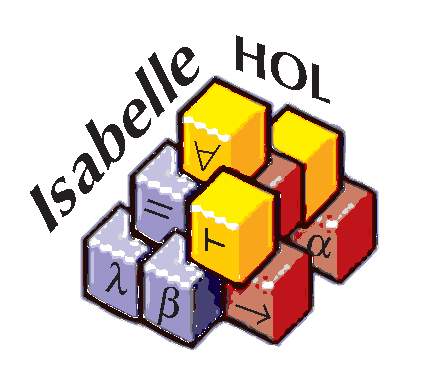
\includegraphics[scale=0.5]{isabelle_hol} \\[4ex]
  Isabelle's Logics: HOL%
  \thanks{The research has been funded by the EPSRC (grants GR/G53279,
    GR\slash H40570, GR/K57381, GR/K77051, GR/M75440), by ESPRIT (projects 3245:
    Logical Frameworks, and 6453: Types) and by the DFG Schwerpunktprogramm
    \emph{Deduktion}.}}

\author{Tobias Nipkow\footnote
{Institut f\"ur Informatik, Technische Universit\"at M\"unchen,
 \texttt{nipkow@in.tum.de}} and
Lawrence C. Paulson\footnote
{Computer Laboratory, University of Cambridge, \texttt{lcp@cl.cam.ac.uk}} and
Markus Wenzel\footnote
{Institut f\"ur Informatik, Technische Universit\"at M\"unchen,
 \texttt{wenzelm@in.tum.de}}}

\newcommand\subcaption[1]{\par {\centering\normalsize\sc#1\par}\bigskip
  \hrule\bigskip}
\newenvironment{constants}{\begin{center}\small\begin{tabular}{rrrr}}{\end{tabular}\end{center}}

\newcommand\bs{\char '134 }  % A backslash character for \tt font

\makeindex

\underscoreoff

\setcounter{secnumdepth}{2} \setcounter{tocdepth}{2}  %% {secnumdepth}{2}???

\pagestyle{headings}
\sloppy
\binperiod     %%%treat . like a binary operator

\begin{document}
\maketitle 

\begin{abstract}
  This manual describes Isabelle's formalization of Higher-Order Logic, a
  polymorphic version of Church's Simple Theory of Types.  HOL can be best
  understood as a simply-typed version of classical set theory.  The monograph
  \emph{Isabelle/HOL --- A Proof Assistant for Higher-Order Logic} provides a
  gentle introduction on using Isabelle/HOL in practice.
\end{abstract}

\pagenumbering{roman} \tableofcontents \clearfirst

\chapter{Syntax primitives}

The rather generic framework of Isabelle/Isar syntax emerges from three main
syntactic categories: \emph{commands} of the top-level Isar engine (covering
theory and proof elements), \emph{methods} for general goal refinements
(analogous to traditional ``tactics''), and \emph{attributes} for operations
on facts (within a certain context).  Here we give a reference of basic
syntactic entities underlying Isabelle/Isar syntax in a bottom-up manner.
Concrete theory and proof language elements will be introduced later on.

\medskip

In order to get started with writing well-formed Isabelle/Isar documents, the
most important aspect to be noted is the difference of \emph{inner} versus
\emph{outer} syntax.  Inner syntax is that of Isabelle types and terms of the
logic, while outer syntax is that of Isabelle/Isar theory sources (including
proofs).  As a general rule, inner syntax entities may occur only as
\emph{atomic entities} within outer syntax.  For example, the string
\texttt{"x + y"} and identifier \texttt{z} are legal term specifications
within a theory, while \texttt{x + y} is not.

\begin{warn}
  Old-style Isabelle theories used to fake parts of the inner syntax of types,
  with rather complicated rules when quotes may be omitted.  Despite the minor
  drawback of requiring quotes more often, the syntax of Isabelle/Isar is
  somewhat simpler and more robust in that respect.
\end{warn}

Printed theory documents usually omit quotes to gain readability (this is a
matter of {\LaTeX} macro setup, say via \verb,\isabellestyle,, see also
\cite{isabelle-sys}).  Experienced users of Isabelle/Isar may easily
reconstruct the lost technical information, while mere readers need not care
about quotes at all.

\medskip

Isabelle/Isar input may contain any number of input termination characters
``\texttt{;}'' (semicolon) to separate commands explicitly.  This is
particularly useful in interactive shell sessions to make clear where the
current command is intended to end.  Otherwise, the interpreter loop will
continue to issue a secondary prompt ``\verb,#,'' until an end-of-command is
clearly recognized from the input syntax, e.g.\ encounter of the next command
keyword.

Advanced interfaces such as Proof~General \cite{proofgeneral} do not require
explicit semicolons, the amount of input text is determined automatically by
inspecting the present content of the Emacs text buffer.  In the printed
presentation of Isabelle/Isar documents semicolons are omitted altogether for
readability.

\begin{warn}
  Proof~General requires certain syntax classification tables in order to
  achieve properly synchronized interaction with the Isabelle/Isar process.
  These tables need to be consistent with the Isabelle version and particular
  logic image to be used in a running session (common object-logics may well
  change the outer syntax).  The standard setup should work correctly with any
  of the ``official'' logic images derived from Isabelle/HOL (including HOLCF
  etc.).  Users of alternative logics may need to tell Proof~General
  explicitly, e.g.\ by giving an option \verb,-k ZF, (in conjunction with
  \verb,-l ZF, to specify the default logic image).
\end{warn}

\section{Lexical matters}\label{sec:lex-syntax}

The Isabelle/Isar outer syntax provides token classes as presented below; most
of these coincide with the inner lexical syntax as presented in
\cite{isabelle-ref}.

\indexoutertoken{ident}\indexoutertoken{longident}\indexoutertoken{symident}
\indexoutertoken{nat}\indexoutertoken{var}\indexoutertoken{typefree}
\indexoutertoken{typevar}\indexoutertoken{string}\indexoutertoken{altstring}
\indexoutertoken{verbatim}
\begin{matharray}{rcl}
  ident & = & letter\,quasiletter^* \\
  longident & = & ident (\verb,.,ident)^+ \\
  symident & = & sym^+ ~|~ \verb,\<,ident\verb,>, \\
  nat & = & digit^+ \\
  var & = & ident ~|~ \verb,?,ident ~|~ \verb,?,ident\verb,.,nat \\
  typefree & = & \verb,',ident \\
  typevar & = & typefree ~|~ \verb,?,typefree ~|~ \verb,?,typefree\verb,.,nat \\
  string & = & \verb,", ~\dots~ \verb,", \\
  altstring & = & \backquote ~\dots~ \backquote \\
  verbatim & = & \verb,{*, ~\dots~ \verb,*}, \\[1ex]

  letter & = & latin ~|~ \verb,\<,latin\verb,>, ~|~ \verb,\<,latin\,latin\verb,>, ~|~ greek ~|~ \\
         &   & \verb,\<^isub>, ~|~ \verb,\<^isup>, \\
  quasiletter & = & letter ~|~ digit ~|~ \verb,_, ~|~ \verb,', \\
  latin & = & \verb,a, ~|~ \dots ~|~ \verb,z, ~|~ \verb,A, ~|~ \dots ~|~ \verb,Z, \\
  digit & = & \verb,0, ~|~ \dots ~|~ \verb,9, \\
  sym & = & \verb,!, ~|~ \verb,#, ~|~ \verb,$, ~|~ \verb,%, ~|~ \verb,&, ~|~  %$
   \verb,*, ~|~ \verb,+, ~|~ \verb,-, ~|~ \verb,/, ~|~ \\
  & & \verb,<, ~|~ \verb,=, ~|~ \verb,>, ~|~ \verb,?, ~|~ \texttt{\at} ~|~
  \verb,^, ~|~ \verb,_, ~|~ \verb,|, ~|~ \verb,~, \\
greek & = & \verb,\<alpha>, ~|~ \verb,\<beta>, ~|~ \verb,\<gamma>, ~|~ \verb,\<delta>, ~| \\
      &   & \verb,\<epsilon>, ~|~ \verb,\<zeta>, ~|~ \verb,\<eta>, ~|~ \verb,\<theta>, ~| \\
      &   & \verb,\<iota>, ~|~ \verb,\<kappa>, ~|~ \verb,\<mu>, ~|~ \verb,\<nu>, ~| \\
      &   & \verb,\<xi>, ~|~ \verb,\<pi>, ~|~ \verb,\<rho>, ~|~ \verb,\<sigma>, ~| \\
      &   & \verb,\<tau>, ~|~ \verb,\<upsilon>, ~|~ \verb,\<phi>, ~|~ \verb,\<psi>, ~| \\
      &   & \verb,\<omega>, ~|~ \verb,\<Gamma>, ~|~ \verb,\<Delta>, ~|~ \verb,\<Theta>, ~| \\
      &   & \verb,\<Lambda>, ~|~ \verb,\<Xi>, ~|~ \verb,\<Pi>, ~|~ \verb,\<Sigma>, ~| \\
      &   & \verb,\<Upsilon>, ~|~ \verb,\<Phi>, ~|~ \verb,\<Psi>, ~|~ \verb,\<Omega>, \\
\end{matharray}

The syntax of $string$ admits any characters, including newlines; ``\verb|"|''
(double-quote) and ``\verb|\|'' (backslash) need to be escaped by a backslash.
Alternative strings according to $altstring$ are analogous, using single
back-quotes instead.  The body of $verbatim$ may consist of any text not
containing ``\verb|*}|''; this allows convenient inclusion of quotes without
further escapes.  The greek letters do \emph{not} include \verb,\<lambda>,,
which is already used differently in the meta-logic.

Common mathematical symbols such as $\forall$ are represented in Isabelle as
\verb,\<forall>,.  There are infinitely many legal symbols like this, although
proper presentation is left to front-end tools such as {\LaTeX} or
Proof~General with the X-Symbol package.  A list of standard Isabelle symbols
that work well with these tools is given in \cite[appendix~A]{isabelle-sys}.

Comments take the form \texttt{(*~\dots~*)} and may be nested, although
user-interface tools may prevent this.  Note that \texttt{(*~\dots~*)}
indicate source comments only, which are stripped after lexical analysis of
the input.  The Isar document syntax also provides formal comments that are
considered as part of the text (see \S\ref{sec:comments}).

\begin{warn}
  Proof~General does not handle nested comments properly; it is also unable to
  keep \verb,(*,\,/\,\verb,{*, and \verb,*),\,/\,\verb,*}, apart, despite
  their rather different meaning.  These are inherent problems of Emacs
  legacy.  Users should not be overly aggressive about nesting or alternating
  these delimiters.
\end{warn}


\section{Common syntax entities}

Subsequently, we introduce several basic syntactic entities, such as names,
terms, and theorem specifications, which have been factored out of the actual
Isar language elements to be described later.

Note that some of the basic syntactic entities introduced below (e.g.\
\railqtok{name}) act much like tokens rather than plain nonterminals (e.g.\
\railnonterm{sort}), especially for the sake of error messages.  E.g.\ syntax
elements like $\CONSTS$ referring to \railqtok{name} or \railqtok{type} would
really report a missing name or type rather than any of the constituent
primitive tokens such as \railtok{ident} or \railtok{string}.


\subsection{Names}

Entity \railqtok{name} usually refers to any name of types, constants,
theorems etc.\ that are to be \emph{declared} or \emph{defined} (so qualified
identifiers are excluded here).  Quoted strings provide an escape for
non-identifier names or those ruled out by outer syntax keywords (e.g.\
\verb|"let"|).  Already existing objects are usually referenced by
\railqtok{nameref}.

\indexoutertoken{name}\indexoutertoken{parname}\indexoutertoken{nameref}
\indexoutertoken{int}
\begin{rail}
  name: ident | symident | string | nat
  ;
  parname: '(' name ')'
  ;
  nameref: name | longident
  ;
  int: nat | '-' nat
  ;
\end{rail}


\subsection{Comments}\label{sec:comments}

Large chunks of plain \railqtok{text} are usually given \railtok{verbatim},
i.e.\ enclosed in \verb|{*|~\dots~\verb|*}|.  For convenience, any of the
smaller text units conforming to \railqtok{nameref} are admitted as well.  A
marginal \railnonterm{comment} is of the form \texttt{--} \railqtok{text}.
Any number of these may occur within Isabelle/Isar commands.

\indexoutertoken{text}\indexouternonterm{comment}
\begin{rail}
  text: verbatim | nameref
  ;
  comment: '--' text
  ;
\end{rail}


\subsection{Type classes, sorts and arities}

Classes are specified by plain names.  Sorts have a very simple inner syntax,
which is either a single class name $c$ or a list $\{c@1, \dots, c@n\}$
referring to the intersection of these classes.  The syntax of type arities is
given directly at the outer level.

\railalias{subseteq}{\isasymsubseteq}
\railterm{subseteq}

\indexouternonterm{sort}\indexouternonterm{arity}
\indexouternonterm{classdecl}
\begin{rail}
  classdecl: name (('<' | subseteq) (nameref + ','))?
  ;
  sort: nameref
  ;
  arity: ('(' (sort + ',') ')')? sort
  ;
\end{rail}


\subsection{Types and terms}\label{sec:types-terms}

The actual inner Isabelle syntax, that of types and terms of the logic, is far
too sophisticated in order to be modelled explicitly at the outer theory
level.  Basically, any such entity has to be quoted to turn it into a single
token (the parsing and type-checking is performed internally later).  For
convenience, a slightly more liberal convention is adopted: quotes may be
omitted for any type or term that is already atomic at the outer level.  For
example, one may just write \texttt{x} instead of \texttt{"x"}.  Note that
symbolic identifiers (e.g.\ \texttt{++} or $\forall$) are available as well,
provided these have not been superseded by commands or other keywords already
(e.g.\ \texttt{=} or \texttt{+}).

\indexoutertoken{type}\indexoutertoken{term}\indexoutertoken{prop}
\begin{rail}
  type: nameref | typefree | typevar
  ;
  term: nameref | var
  ;
  prop: term
  ;
\end{rail}

Positional instantiations are indicated by giving a sequence of terms, or the
placeholder ``$\_$'' (underscore), which means to skip a position.

\indexoutertoken{inst}\indexoutertoken{insts}
\begin{rail}
  inst: underscore | term
  ;
  insts: (inst *)
  ;
\end{rail}

Type declarations and definitions usually refer to \railnonterm{typespec} on
the left-hand side.  This models basic type constructor application at the
outer syntax level.  Note that only plain postfix notation is available here,
but no infixes.

\indexouternonterm{typespec}
\begin{rail}
  typespec: (() | typefree | '(' ( typefree + ',' ) ')') name
  ;
\end{rail}


\subsection{Mixfix annotations}

Mixfix annotations specify concrete \emph{inner} syntax of Isabelle types and
terms.  Some commands such as $\TYPES$ (see \S\ref{sec:types-pure}) admit
infixes only, while $\CONSTS$ (see \S\ref{sec:consts}) and
$\isarkeyword{syntax}$ (see \S\ref{sec:syn-trans}) support the full range of
general mixfixes and binders.

\indexouternonterm{infix}\indexouternonterm{mixfix}\indexouternonterm{structmixfix}
\begin{rail}
  infix: '(' ('infix' | 'infixl' | 'infixr') string? nat ')'
  ;
  mixfix: infix | '(' string prios? nat? ')' | '(' 'binder' string prios? nat ')'
  ;
  structmixfix: mixfix | '(' 'structure' ')'
  ;

  prios: '[' (nat + ',') ']'
  ;
\end{rail}

Here the \railtok{string} specifications refer to the actual mixfix template
(see also \cite{isabelle-ref}), which may include literal text, spacing,
blocks, and arguments (denoted by ``$_$''); the special symbol \verb,\<index>,
(printed as ``\i'') represents an index argument that specifies an implicit
structure reference (see also \S\ref{sec:locale}).  Infix and binder
declarations provide common abbreviations for particular mixfix declarations.
So in practice, mixfix templates mostly degenerate to literal text for
concrete syntax, such as ``\verb,++,'' for an infix symbol, or ``\verb,++,\i''
for an infix of an implicit structure.



\subsection{Proof methods}\label{sec:syn-meth}

Proof methods are either basic ones, or expressions composed of
methods via ``\texttt{,}'' (sequential composition), ``\texttt{|}''
(alternative choices), ``\texttt{?}'' (try), ``\texttt{+}'' (repeat at
least once), ``\texttt{[$n$]}'' (restriction to first $n$ sub-goals,
default $n = 1$).  In practice, proof methods are usually just a comma
separated list of \railqtok{nameref}~\railnonterm{args}
specifications.  Note that parentheses may be dropped for single
method specifications (with no arguments).

\indexouternonterm{method}
\begin{rail}
  method: (nameref | '(' methods ')') (() | '?' | '+' | '[' nat? ']')
  ;
  methods: (nameref args | method) + (',' | '|')
  ;
\end{rail}

Proper Isar proof methods do \emph{not} admit arbitrary goal
addressing, but refer either to the first sub-goal or all sub-goals
uniformly.  The goal restriction operator ``\texttt{[$n$]}'' evaluates
a method expression within a sandbox consisting of the first $n$
sub-goals (which need to exist).  For example,
$simp_all\mbox{\tt[}3\mbox{\tt]}$ simplifies the first three
sub-goals, while $(rule~foo, simp_all)\mbox{\tt[]}$ simplifies all new
goals that emerge from applying rule $foo$ to the originally first
one.

Improper methods, notably tactic emulations, offer a separate
low-level goal addressing scheme as explicit argument to the
individual tactic being involved.  Here $[!]$ refers to all goals, and
$[n-]$ to all goals starting from $n$,

\indexouternonterm{goalspec}
\begin{rail}
  goalspec: '[' (nat '-' nat | nat '-' | nat | '!' ) ']'
  ;
\end{rail}


\subsection{Attributes and theorems}\label{sec:syn-att}

Attributes (and proof methods, see \S\ref{sec:syn-meth}) have their own
``semi-inner'' syntax, in the sense that input conforming to
\railnonterm{args} below is parsed by the attribute a second time.  The
attribute argument specifications may be any sequence of atomic entities
(identifiers, strings etc.), or properly bracketed argument lists.  Below
\railqtok{atom} refers to any atomic entity, including any \railtok{keyword}
conforming to \railtok{symident}.

\indexoutertoken{atom}\indexouternonterm{args}\indexouternonterm{attributes}
\begin{rail}
  atom: nameref | typefree | typevar | var | nat | keyword
  ;
  arg: atom | '(' args ')' | '[' args ']'
  ;
  args: arg *
  ;
  attributes: '[' (nameref args * ',') ']'
  ;
\end{rail}

Theorem specifications come in several flavors: \railnonterm{axmdecl} and
\railnonterm{thmdecl} usually refer to axioms, assumptions or results of goal
statements, while \railnonterm{thmdef} collects lists of existing theorems.
Existing theorems are given by \railnonterm{thmref} and \railnonterm{thmrefs},
the former requires an actual singleton result.  There are three forms of
theorem references: (1) named facts $a$, (2) selections from named facts $a(i,
j - k)$, or (3) literal fact propositions using $altstring$ syntax
$\backquote\phi\backquote$, (see also method $fact$ in
\S\ref{sec:pure-meth-att}).

Any kind of theorem specification may include lists of attributes both on the
left and right hand sides; attributes are applied to any immediately preceding
fact.  If names are omitted, the theorems are not stored within the theorem
database of the theory or proof context, but any given attributes are applied
nonetheless.

\indexouternonterm{axmdecl}\indexouternonterm{thmdecl}
\indexouternonterm{thmdef}\indexouternonterm{thmref}
\indexouternonterm{thmrefs}\indexouternonterm{selection}
\begin{rail}
  axmdecl: name attributes? ':'
  ;
  thmdecl: thmbind ':'
  ;
  thmdef: thmbind '='
  ;
  thmref: (nameref selection? | altstring) attributes?
  ;
  thmrefs: thmref +
  ;

  thmbind: name attributes | name | attributes
  ;
  selection: '(' ((nat | nat '-' nat?) + ',') ')'
  ;
\end{rail}


\subsection{Term patterns and declarations}\label{sec:term-decls}

Wherever explicit propositions (or term fragments) occur in a proof text,
casual binding of schematic term variables may be given specified via patterns
of the form ``$\ISS{p@1\;\dots}{p@n}$''.  There are separate versions
available for \railqtok{term}s and \railqtok{prop}s.  The latter provides a
$\CONCLNAME$ part with patterns referring the (atomic) conclusion of a rule.

\indexouternonterm{termpat}\indexouternonterm{proppat}
\begin{rail}
  termpat: '(' ('is' term +) ')'
  ;
  proppat: '(' ('is' prop +) ')'
  ;
\end{rail}

Declarations of local variables $x :: \tau$ and logical propositions $a :
\phi$ represent different views on the same principle of introducing a local
scope.  In practice, one may usually omit the typing of $vars$ (due to
type-inference), and the naming of propositions (due to implicit references of
current facts).  In any case, Isar proof elements usually admit to introduce
multiple such items simultaneously.

\indexouternonterm{vars}\indexouternonterm{props}
\begin{rail}
  vars: (name+) ('::' type)?
  ;
  props: thmdecl? (prop proppat? +)
  ;
\end{rail}

The treatment of multiple declarations corresponds to the complementary focus
of $vars$ versus $props$: in ``$x@1~\dots~x@n :: \tau$'' the typing refers to
all variables, while in $a\colon \phi@1~\dots~\phi@n$ the naming refers to all
propositions collectively.  Isar language elements that refer to $vars$ or
$props$ typically admit separate typings or namings via another level of
iteration, with explicit $\AND$ separators; e.g.\ see $\FIXNAME$ and
$\ASSUMENAME$ in \S\ref{sec:proof-context}.


\subsection{Antiquotations}\label{sec:antiq}

\begin{matharray}{rcl}
  theory & : & \isarantiq \\
  thm & : & \isarantiq \\
  prop & : & \isarantiq \\
  term & : & \isarantiq \\
  const & : & \isarantiq \\
  abbrev & : & \isarantiq \\
  typeof & : & \isarantiq \\
  typ & : & \isarantiq \\
  thm_style & : & \isarantiq \\
  term_style & : & \isarantiq \\
  text & : & \isarantiq \\
  goals & : & \isarantiq \\
  subgoals & : & \isarantiq \\
  prf & : & \isarantiq \\
  full_prf & : & \isarantiq \\
  ML & : & \isarantiq \\
  ML_type & : & \isarantiq \\
  ML_struct & : & \isarantiq \\
\end{matharray}

The text body of formal comments (see also \S\ref{sec:comments}) may contain
antiquotations of logical entities, such as theorems, terms and types, which
are to be presented in the final output produced by the Isabelle document
preparation system (see also \S\ref{sec:document-prep}).

Thus embedding of
``\texttt{{\at}{\ttlbrace}term~[show_types]~"f(x)~=~a~+~x"{\ttrbrace}}''
within a text block would cause
\isa{(f{\isasymColon}'a~{\isasymRightarrow}~'a)~(x{\isasymColon}'a)~=~(a{\isasymColon}'a)~+~x}
to appear in the final {\LaTeX} document.  Also note that theorem
antiquotations may involve attributes as well.  For example,
\texttt{{\at}{\ttlbrace}thm~sym~[no_vars]{\ttrbrace}} would print the
statement where all schematic variables have been replaced by fixed ones,
which are easier to read.

\indexisarant{theory}\indexisarant{thm}\indexisarant{prop}\indexisarant{term}\indexisarant{const}
\indexisarant{abbrev}\indexisarant{typeof}\indexisarant{typ}\indexisarant{thm-style}
\indexisarant{term-style}\indexisarant{text}\indexisarant{goals}
\indexisarant{subgoals}\indexisarant{prf}\indexisarant{full-prf}\indexisarant{ML}
\indexisarant{ML-type}\indexisarant{ML-struct}

\begin{rail}
  atsign lbrace antiquotation rbrace
  ;

  antiquotation:
    'theory' options name |
    'thm' options thmrefs |
    'prop' options prop |
    'term' options term |
    'const' options term |
    'abbrev' options term |
    'typeof' options term |
    'typ' options type |
    'thm\_style' options name thmref |
    'term\_style' options name term |
    'text' options name |
    'goals' options |
    'subgoals' options |
    'prf' options thmrefs |
    'full\_prf' options thmrefs |
    'ML' options name |
    'ML\_type' options name |
    'ML\_struct' options name
  ;
  options: '[' (option * ',') ']'
  ;
  option: name | name '=' name
  ;
\end{rail}

Note that the syntax of antiquotations may \emph{not} include source comments
\texttt{(*~\dots~*)} or verbatim text \verb|{*|~\dots~\verb|*}|.

\begin{descr}
  
\item [$\at\{theory~A\}$] prints the name $A$, which is guaranteed to
  refer to a valid ancestor theory in the current context.

\item [$\at\{thm~\vec a\}$] prints theorems $\vec a$. Note that attribute
  specifications may be included as well (see also \S\ref{sec:syn-att}); the
  $no_vars$ operation (see \S\ref{sec:misc-meth-att}) would be particularly
  useful to suppress printing of schematic variables.

\item [$\at\{prop~\phi\}$] prints a well-typed proposition $\phi$.

\item [$\at\{term~t\}$] prints a well-typed term $t$.

\item [$\at\{const~c\}$] prints a well-defined constant $c$.
  
\item [$\at\{abbrev~c\,\vec x\}$] prints a constant abbreviation
  $c\,\vec x \equiv rhs$ as defined in the current context.

\item [$\at\{typeof~t\}$] prints the type of a well-typed term $t$.

\item [$\at\{typ~\tau\}$] prints a well-formed type $\tau$.
  
\item [$\at\{thm_style~s~a\}$] prints theorem $a$, previously applying a style
  $s$ to it (see below).
  
\item [$\at\{term_style~s~t\}$] prints a well-typed term $t$ after applying a
  style $s$ to it (see below).

\item [$\at\{text~s\}$] prints uninterpreted source text $s$.  This is
  particularly useful to print portions of text according to the Isabelle
  {\LaTeX} output style, without demanding well-formedness (e.g.\ small pieces
  of terms that should not be parsed or type-checked yet).

\item [$\at\{goals\}$] prints the current \emph{dynamic} goal state.  This is
  mainly for support of tactic-emulation scripts within Isar --- presentation
  of goal states does not conform to actual human-readable proof documents.
  Please do not include goal states into document output unless you really
  know what you are doing!
  
\item [$\at\{subgoals\}$] is similar to $goals$, but does not print the main
  goal.
  
\item [$\at\{prf~\vec a\}$] prints the (compact) proof terms corresponding to
  the theorems $\vec a$. Note that this requires proof terms to be switched on
  for the current object logic (see the ``Proof terms'' section of the
  Isabelle reference manual for information on how to do this).
  
\item [$\at\{full_prf~\vec a\}$] is like $\at\{prf~\vec a\}$, but displays the
  full proof terms, i.e.\ also displays information omitted in the compact
  proof term, which is denoted by ``$_$'' placeholders there.
  
\item [$\at\{ML~s\}$, $\at\{ML_type~s\}$, and $\at\{ML_struct~s\}$] check text
  $s$ as ML value, type, and structure, respectively.  If successful, the
  source is displayed verbatim.

\end{descr}

\medskip

The following standard styles for use with $thm_style$ and $term_style$ are
available:

\begin{descr}
  
\item [$lhs$] extracts the first argument of any application form with at
  least two arguments -- typically meta-level or object-level equality, or any
  other binary relation.
  
\item [$rhs$] is like $lhs$, but extracts the second argument.
  
\item [$concl$] extracts the conclusion $C$ from a nested meta-level
  implication $A@1 \Imp \cdots A@n \Imp C$.
  
\item [$prem1$, \dots, $prem9$] extract premise number $1$, \dots, $9$,
  respectively, from a nested meta-level implication $A@1 \Imp \cdots A@n \Imp
  C$.

\end{descr}

\medskip

The following options are available to tune the output.  Note that most of
these coincide with ML flags of the same names (see also \cite{isabelle-ref}).
\begin{descr}
\item[$show_types = bool$ and $show_sorts = bool$] control printing of
  explicit type and sort constraints.
\item[$show_structs = bool$] controls printing of implicit structures.
\item[$long_names = bool$] forces names of types and constants etc.\ to be
  printed in their fully qualified internal form.
\item[$short_names = bool$] forces names of types and constants etc.\ to be
  printed unqualified.  Note that internalizing the output again in the
  current context may well yield a different result.
\item[$unique_names = bool$] determines whether the printed version of
  qualified names should be made sufficiently long to avoid overlap with names
  declared further back.  Set to $false$ for more concise output.
\item[$eta_contract = bool$] prints terms in $\eta$-contracted form.
\item[$display = bool$] indicates if the text is to be output as multi-line
  ``display material'', rather than a small piece of text without line breaks
  (which is the default).
\item[$breaks = bool$] controls line breaks in non-display material.
\item[$quotes = bool$] indicates if the output should be enclosed in double
  quotes.
\item[$mode = name$] adds $name$ to the print mode to be used for presentation
  (see also \cite{isabelle-ref}).  Note that the standard setup for {\LaTeX}
  output is already present by default, including the modes ``$latex$'',
  ``$xsymbols$'', ``$symbols$''.
\item[$margin = nat$ and $indent = nat$] change the margin or indentation for
  pretty printing of display material.
\item[$source = bool$] prints the source text of the antiquotation arguments,
  rather than the actual value.  Note that this does not affect
  well-formedness checks of $thm$, $term$, etc. (only the $text$ antiquotation
  admits arbitrary output).
\item[$goals_limit = nat$] determines the maximum number of goals to be
  printed.
\item[$locale = name$] specifies an alternative context used for evaluating
  and printing the subsequent argument.
\end{descr}

For boolean flags, ``$name = true$'' may be abbreviated as ``$name$''.  All of
the above flags are disabled by default, unless changed from ML.

\medskip Note that antiquotations do not only spare the author from tedious
typing of logical entities, but also achieve some degree of
consistency-checking of informal explanations with formal developments:
well-formedness of terms and types with respect to the current theory or proof
context is ensured here.


\subsection{Tagged commands}\label{sec:tags}

Each Isabelle/Isar command may be decorated by presentation tags:

\indexouternonterm{tags}
\begin{rail}
  tags: ( tag * )
  ;
  tag: '\%' (ident | string)
\end{rail}

The tags $theory$, $proof$, $ML$ are already pre-declared for certain classes
of commands:

\medskip

\begin{tabular}{ll}
  $theory$ & theory begin and end \\
  $proof$ & all proof commands \\
  $ML$ & all commands involving ML code \\
\end{tabular}

\medskip The Isabelle document preparation system (see also
\cite{isabelle-sys}) allows tagged command regions to be presented
specifically, e.g.\ to fold proof texts, or drop parts of the text completely.

For example ``$\BYNAME~\%invisible~(auto)$'' would cause that piece of proof
to be treated as $invisible$ instead of $proof$ (the default), which may be
either show or hidden depending on the document setup.  In contrast,
``$\BYNAME~\%visible~(auto)$'' would force this text to be shown invariably.

Explicit tag specifications within a proof apply to all subsequent commands of
the same level of nesting.  For example,
``$\PROOFNAME~\%visible~\dots\QEDNAME$'' would force the whole sub-proof to be
typeset as $visible$ (unless some of its parts are tagged differently).

%%% Local Variables:
%%% mode: latex
%%% TeX-master: "isar-ref"
%%% End:

%% $Id$
\chapter{Higher-Order Logic}
\index{higher-order logic|(}
\index{HOL system@{\sc hol} system}

The theory~\thydx{HOL} implements higher-order logic.  It is based on
Gordon's~{\sc hol} system~\cite{mgordon-hol}, which itself is based on
Church's original paper~\cite{church40}.  Andrews's
book~\cite{andrews86} is a full description of the original
Church-style higher-order logic.  Experience with the {\sc hol} system
has demonstrated that higher-order logic is widely applicable in many
areas of mathematics and computer science, not just hardware
verification, {\sc hol}'s original {\it raison d'\^etre\/}.  It is
weaker than {\ZF} set theory but for most applications this does not
matter.  If you prefer {\ML} to Lisp, you will probably prefer \HOL\ 
to~{\ZF}.

The syntax of \HOL\footnote{Earlier versions of Isabelle's \HOL\ used a
different syntax. Ancient releases of Isabelle included still another version
of~\HOL, with explicit type inference rules~\cite{paulson-COLOG}.  This
version no longer exists, but \thydx{ZF} supports a similar style of
reasoning.} follows $\lambda$-calculus and functional programming.  Function
application is curried.  To apply the function~$f$ of type
$\tau@1\To\tau@2\To\tau@3$ to the arguments~$a$ and~$b$ in \HOL, you simply
write $f\,a\,b$. There is no `apply' operator as in \thydx{ZF}. Note that
$f(a,b)$ means ``$f$ applied to the pair $(a,b)$'' in \HOL.  We write ordered
pairs as $(a,b)$, not $\langle a,b\rangle$ as in {\ZF}.

\HOL\ has a distinct feel, compared with {\ZF} and {\CTT}.  It
identifies object-level types with meta-level types, taking advantage of
Isabelle's built-in type checker.  It identifies object-level functions
with meta-level functions, so it uses Isabelle's operations for abstraction
and application.

These identifications allow Isabelle to support \HOL\ particularly
nicely, but they also mean that \HOL\ requires more sophistication
from the user --- in particular, an understanding of Isabelle's type
system.  Beginners should work with {\tt show_types} (or even
\texttt{show_sorts}) set to {\tt true}.
%  Gain experience by
%working in first-order logic before attempting to use higher-order logic.
%This chapter assumes familiarity with~{\FOL{}}.


\begin{figure}
\begin{constants}
  \it name      &\it meta-type  & \it description \\
  \cdx{Trueprop}& $bool\To prop$                & coercion to $prop$\\
  \cdx{Not}     & $bool\To bool$                & negation ($\neg$) \\
  \cdx{True}    & $bool$                        & tautology ($\top$) \\
  \cdx{False}   & $bool$                        & absurdity ($\bot$) \\
  \cdx{If}      & $[bool,\alpha,\alpha]\To\alpha$ & conditional \\
  \cdx{Let}     & $[\alpha,\alpha\To\beta]\To\beta$ & let binder
\end{constants}
\subcaption{Constants}

\begin{constants}
\index{"@@{\tt\at} symbol}
\index{*"! symbol}\index{*"? symbol}
\index{*"?"! symbol}\index{*"E"X"! symbol}
  \it symbol &\it name     &\it meta-type & \it description \\
  \tt\at & \cdx{Eps}  & $(\alpha\To bool)\To\alpha$ & 
        Hilbert description ($\varepsilon$) \\
  {\tt!~} or \sdx{ALL}  & \cdx{All}  & $(\alpha\To bool)\To bool$ & 
        universal quantifier ($\forall$) \\
  {\tt?~} or \sdx{EX}   & \cdx{Ex}   & $(\alpha\To bool)\To bool$ & 
        existential quantifier ($\exists$) \\
  {\tt?!} or {\tt EX!}  & \cdx{Ex1}  & $(\alpha\To bool)\To bool$ & 
        unique existence ($\exists!$)\\
  {\tt LEAST}  & \cdx{Least}  & $(\alpha::ord \To bool)\To\alpha$ & 
        least element
\end{constants}
\subcaption{Binders} 

\begin{constants}
\index{*"= symbol}
\index{&@{\tt\&} symbol}
\index{*"| symbol}
\index{*"-"-"> symbol}
  \it symbol    & \it meta-type & \it priority & \it description \\ 
  \sdx{o}       & $[\beta\To\gamma,\alpha\To\beta]\To (\alpha\To\gamma)$ & 
        Left 55 & composition ($\circ$) \\
  \tt =         & $[\alpha,\alpha]\To bool$ & Left 50 & equality ($=$) \\
  \tt <         & $[\alpha::ord,\alpha]\To bool$ & Left 50 & less than ($<$) \\
  \tt <=        & $[\alpha::ord,\alpha]\To bool$ & Left 50 & 
                less than or equals ($\leq$)\\
  \tt \&        & $[bool,bool]\To bool$ & Right 35 & conjunction ($\conj$) \\
  \tt |         & $[bool,bool]\To bool$ & Right 30 & disjunction ($\disj$) \\
  \tt -->       & $[bool,bool]\To bool$ & Right 25 & implication ($\imp$)
\end{constants}
\subcaption{Infixes}
\caption{Syntax of {\tt HOL}} \label{hol-constants}
\end{figure}


\begin{figure}
\index{*let symbol}
\index{*in symbol}
\dquotes
\[\begin{array}{rclcl}
    term & = & \hbox{expression of class~$term$} \\
         & | & "\at~" id " . " formula \\
         & | & 
    \multicolumn{3}{l}{"let"~id~"="~term";"\dots";"~id~"="~term~"in"~term} \\
         & | & 
    \multicolumn{3}{l}{"if"~formula~"then"~term~"else"~term} \\
         & | & "LEAST"~ id " . " formula \\[2ex]
 formula & = & \hbox{expression of type~$bool$} \\
         & | & term " = " term \\
         & | & term " \ttilde= " term \\
         & | & term " < " term \\
         & | & term " <= " term \\
         & | & "\ttilde\ " formula \\
         & | & formula " \& " formula \\
         & | & formula " | " formula \\
         & | & formula " --> " formula \\
         & | & "!~~~" id~id^* " . " formula 
         & | & "ALL~" id~id^* " . " formula \\
         & | & "?~~~" id~id^* " . " formula 
         & | & "EX~~" id~id^* " . " formula \\
         & | & "?!~~" id~id^* " . " formula 
         & | & "EX!~" id~id^* " . " formula
  \end{array}
\]
\caption{Full grammar for \HOL} \label{hol-grammar}
\end{figure} 


\section{Syntax}

Figure~\ref{hol-constants} lists the constants (including infixes and
binders), while Fig.\ts\ref{hol-grammar} presents the grammar of
higher-order logic.  Note that $a$\verb|~=|$b$ is translated to
$\neg(a=b)$.

\begin{warn}
  \HOL\ has no if-and-only-if connective; logical equivalence is expressed
  using equality.  But equality has a high priority, as befitting a
  relation, while if-and-only-if typically has the lowest priority.  Thus,
  $\neg\neg P=P$ abbreviates $\neg\neg (P=P)$ and not $(\neg\neg P)=P$.
  When using $=$ to mean logical equivalence, enclose both operands in
  parentheses.
\end{warn}

\subsection{Types and classes}
The universal type class of higher-order terms is called~\cldx{term}.
By default, explicit type variables have class \cldx{term}.  In
particular the equality symbol and quantifiers are polymorphic over
class {\tt term}.

The type of formulae, \tydx{bool}, belongs to class \cldx{term}; thus,
formulae are terms.  The built-in type~\tydx{fun}, which constructs
function types, is overloaded with arity {\tt(term,\thinspace
  term)\thinspace term}.  Thus, $\sigma\To\tau$ belongs to class~{\tt
  term} if $\sigma$ and~$\tau$ do, allowing quantification over
functions.

\HOL\ offers various methods for introducing new types.
See~\S\ref{sec:HOL:Types} and~\S\ref{sec:HOL:datatype}.

Theory \thydx{Ord} defines the syntactic class \cldx{ord} of order
signatures; the relations $<$ and $\leq$ are polymorphic over this
class, as are the functions \cdx{mono}, \cdx{min} and \cdx{max}, and
the \cdx{LEAST} operator. \thydx{Ord} also defines a subclass
\cldx{order} of \cldx{ord} which axiomatizes partially ordered types
(w.r.t.\ $\le$).

Three other syntactic type classes --- \cldx{plus}, \cldx{minus} and
\cldx{times} --- permit overloading of the operators {\tt+},\index{*"+
  symbol} {\tt-}\index{*"- symbol} and {\tt*}.\index{*"* symbol} In
particular, {\tt-} is instantiated for set difference and subtraction
on natural numbers.

If you state a goal containing overloaded functions, you may need to include
type constraints.  Type inference may otherwise make the goal more
polymorphic than you intended, with confusing results. For example, the
variables $i$, $j$ and $k$ in the goal $i \le j \Imp i \le j+k$ have type
$\alpha::\{ord,plus\}$, although you may have expected them to have some
numeric type, e.g. $nat$. Instead you should have stated the goal as
$(i::nat) \le j \Imp i \le j+k$, which causes all three variables to have
type $nat$.

\begin{warn}
  If resolution fails for no obvious reason, try setting
  \ttindex{show_types} to {\tt true}, causing Isabelle to display
  types of terms.  Possibly set \ttindex{show_sorts} to {\tt true} as
  well, causing Isabelle to display type classes and sorts.

  \index{unification!incompleteness of}
  Where function types are involved, Isabelle's unification code does not
  guarantee to find instantiations for type variables automatically.  Be
  prepared to use \ttindex{res_inst_tac} instead of {\tt resolve_tac},
  possibly instantiating type variables.  Setting
  \ttindex{Unify.trace_types} to {\tt true} causes Isabelle to report
  omitted search paths during unification.\index{tracing!of unification}
\end{warn}


\subsection{Binders}

Hilbert's {\bf description} operator~$\varepsilon x.P[x]$ stands for
some~$x$ satisfying~$P$, if such exists.  Since all terms in \HOL\ 
denote something, a description is always meaningful, but we do not
know its value unless $P$ defines it uniquely.  We may write
descriptions as \cdx{Eps}($\lambda x.P[x]$) or use the syntax
\hbox{\tt \at $x$.$P[x]$}.

Existential quantification is defined by
\[ \exists x.P~x \;\equiv\; P(\varepsilon x.P~x). \]
The unique existence quantifier, $\exists!x.P$, is defined in terms
of~$\exists$ and~$\forall$.  An Isabelle binder, it admits nested
quantifications.  For instance, $\exists!x\,y.P\,x\,y$ abbreviates
$\exists!x. \exists!y.P\,x\,y$; note that this does not mean that there
exists a unique pair $(x,y)$ satisfying~$P\,x\,y$.

\index{*"! symbol}\index{*"? symbol}\index{HOL system@{\sc hol} system}
Quantifiers have two notations.  As in Gordon's {\sc hol} system, \HOL\
uses~{\tt!}\ and~{\tt?}\ to stand for $\forall$ and $\exists$.  The
existential quantifier must be followed by a space; thus {\tt?x} is an
unknown, while \verb'? x.f x=y' is a quantification.  Isabelle's usual
notation for quantifiers, \sdx{ALL} and \sdx{EX}, is also
available.  Both notations are accepted for input.  The {\ML} reference
\ttindexbold{HOL_quantifiers} governs the output notation.  If set to {\tt
true}, then~{\tt!}\ and~{\tt?}\ are displayed; this is the default.  If set
to {\tt false}, then~{\tt ALL} and~{\tt EX} are displayed.

If $\tau$ is a type of class \cldx{ord}, $P$ a formula and $x$ a
variable of type $\tau$, then the term \cdx{LEAST}~$x.P[x]$ is defined
to be the least (w.r.t.\ $\le$) $x$ such that $P~x$ holds (see
Fig.~\ref{hol-defs}). The definition uses Hilbert's $\varepsilon$
choice operator, so \texttt{Least} is always meaningful, but may yield
nothing useful in case there is not a unique least element satisfying
$P$.\footnote{Class $ord$ does not require much of its instances, so
  $\le$ need not be a well-ordering, not even an order at all!}

\medskip All these binders have priority 10.

\begin{warn}
The low priority of binders means that they need to be enclosed in
parenthesis when they occur in the context of other operations. For example,
instead of $P \land \forall x.Q$ you need to write $P \land (\forall x.Q)$.
\end{warn}


\subsection{The \sdx{let} and \sdx{case} constructions}
Local abbreviations can be introduced by a {\tt let} construct whose
syntax appears in Fig.\ts\ref{hol-grammar}.  Internally it is translated into
the constant~\cdx{Let}.  It can be expanded by rewriting with its
definition, \tdx{Let_def}.

\HOL\ also defines the basic syntax
\[\dquotes"case"~e~"of"~c@1~"=>"~e@1~"|" \dots "|"~c@n~"=>"~e@n\] 
as a uniform means of expressing {\tt case} constructs.  Therefore {\tt case}
and \sdx{of} are reserved words.  Initially, this is mere syntax and has no
logical meaning.  By declaring translations, you can cause instances of the
{\tt case} construct to denote applications of particular case operators.
This is what happens automatically for each {\tt datatype} definition
(see~\S\ref{sec:HOL:datatype}).

\begin{warn}
Both {\tt if} and {\tt case} constructs have as low a priority as
quantifiers, which requires additional enclosing parentheses in the context
of most other operations. For example, instead of $f~x = if \dots then \dots
else \dots$ you need to write $f~x = (if \dots then \dots else
\dots)$.
\end{warn}

\section{Rules of inference}

\begin{figure}
\begin{ttbox}\makeatother
\tdx{refl}           t = (t::'a)
\tdx{subst}          [| s = t; P s |] ==> P (t::'a)
\tdx{ext}            (!!x::'a. (f x :: 'b) = g x) ==> (\%x.f x) = (\%x.g x)
\tdx{impI}           (P ==> Q) ==> P-->Q
\tdx{mp}             [| P-->Q;  P |] ==> Q
\tdx{iff}            (P-->Q) --> (Q-->P) --> (P=Q)
\tdx{selectI}        P(x::'a) ==> P(@x.P x)
\tdx{True_or_False}  (P=True) | (P=False)
\end{ttbox}
\caption{The {\tt HOL} rules} \label{hol-rules}
\end{figure}

Figure~\ref{hol-rules} shows the primitive inference rules of~\HOL{},
with their~{\ML} names.  Some of the rules deserve additional
comments:
\begin{ttdescription}
\item[\tdx{ext}] expresses extensionality of functions.
\item[\tdx{iff}] asserts that logically equivalent formulae are
  equal.
\item[\tdx{selectI}] gives the defining property of the Hilbert
  $\varepsilon$-operator.  It is a form of the Axiom of Choice.  The derived rule
  \tdx{select_equality} (see below) is often easier to use.
\item[\tdx{True_or_False}] makes the logic classical.\footnote{In
    fact, the $\varepsilon$-operator already makes the logic classical, as
    shown by Diaconescu; see Paulson~\cite{paulson-COLOG} for details.}
\end{ttdescription}


\begin{figure}\hfuzz=4pt%suppress "Overfull \hbox" message
\begin{ttbox}\makeatother
\tdx{True_def}   True     == ((\%x::bool.x)=(\%x.x))
\tdx{All_def}    All      == (\%P. P = (\%x.True))
\tdx{Ex_def}     Ex       == (\%P. P(@x.P x))
\tdx{False_def}  False    == (!P.P)
\tdx{not_def}    not      == (\%P. P-->False)
\tdx{and_def}    op &     == (\%P Q. !R. (P-->Q-->R) --> R)
\tdx{or_def}     op |     == (\%P Q. !R. (P-->R) --> (Q-->R) --> R)
\tdx{Ex1_def}    Ex1      == (\%P. ? x. P x & (! y. P y --> y=x))

\tdx{o_def}      op o     == (\%(f::'b=>'c) g x::'a. f(g x))
\tdx{if_def}     If P x y ==
              (\%P x y. @z::'a.(P=True --> z=x) & (P=False --> z=y))
\tdx{Let_def}    Let s f  == f s
\tdx{Least_def}  Least P  == @x. P(x) & (ALL y. P(y) --> x <= y)"
\end{ttbox}
\caption{The {\tt HOL} definitions} \label{hol-defs}
\end{figure}


\HOL{} follows standard practice in higher-order logic: only a few
connectives are taken as primitive, with the remainder defined obscurely
(Fig.\ts\ref{hol-defs}).  Gordon's {\sc hol} system expresses the
corresponding definitions \cite[page~270]{mgordon-hol} using
object-equality~({\tt=}), which is possible because equality in
higher-order logic may equate formulae and even functions over formulae.
But theory~\HOL{}, like all other Isabelle theories, uses
meta-equality~({\tt==}) for definitions.
\begin{warn}
The definitions above should never be expanded and are shown for completeness
only. Instead users should reason in terms of the derived rules shown below
or, better still, using high-level tactics
(see~\S\ref{sec:HOL:generic-packages}).
\end{warn}

Some of the rules mention type variables; for example, {\tt refl}
mentions the type variable~{\tt'a}.  This allows you to instantiate
type variables explicitly by calling {\tt res_inst_tac}.


\begin{figure}
\begin{ttbox}
\tdx{sym}         s=t ==> t=s
\tdx{trans}       [| r=s; s=t |] ==> r=t
\tdx{ssubst}      [| t=s; P s |] ==> P t
\tdx{box_equals}  [| a=b;  a=c;  b=d |] ==> c=d  
\tdx{arg_cong}    x = y ==> f x = f y
\tdx{fun_cong}    f = g ==> f x = g x
\tdx{cong}        [| f = g; x = y |] ==> f x = g y
\tdx{not_sym}     t ~= s ==> s ~= t
\subcaption{Equality}

\tdx{TrueI}       True 
\tdx{FalseE}      False ==> P

\tdx{conjI}       [| P; Q |] ==> P&Q
\tdx{conjunct1}   [| P&Q |] ==> P
\tdx{conjunct2}   [| P&Q |] ==> Q 
\tdx{conjE}       [| P&Q;  [| P; Q |] ==> R |] ==> R

\tdx{disjI1}      P ==> P|Q
\tdx{disjI2}      Q ==> P|Q
\tdx{disjE}       [| P | Q; P ==> R; Q ==> R |] ==> R

\tdx{notI}        (P ==> False) ==> ~ P
\tdx{notE}        [| ~ P;  P |] ==> R
\tdx{impE}        [| P-->Q;  P;  Q ==> R |] ==> R
\subcaption{Propositional logic}

\tdx{iffI}        [| P ==> Q;  Q ==> P |] ==> P=Q
\tdx{iffD1}       [| P=Q; P |] ==> Q
\tdx{iffD2}       [| P=Q; Q |] ==> P
\tdx{iffE}        [| P=Q; [| P --> Q; Q --> P |] ==> R |] ==> R
%
%\tdx{eqTrueI}     P ==> P=True 
%\tdx{eqTrueE}     P=True ==> P 
\subcaption{Logical equivalence}

\end{ttbox}
\caption{Derived rules for \HOL} \label{hol-lemmas1}
\end{figure}


\begin{figure}
\begin{ttbox}\makeatother
\tdx{allI}      (!!x. P x) ==> !x. P x
\tdx{spec}      !x.P x ==> P x
\tdx{allE}      [| !x.P x;  P x ==> R |] ==> R
\tdx{all_dupE}  [| !x.P x;  [| P x; !x.P x |] ==> R |] ==> R

\tdx{exI}       P x ==> ? x. P x
\tdx{exE}       [| ? x. P x; !!x. P x ==> Q |] ==> Q

\tdx{ex1I}      [| P a;  !!x. P x ==> x=a |] ==> ?! x. P x
\tdx{ex1E}      [| ?! x.P x;  !!x. [| P x;  ! y. P y --> y=x |] ==> R 
          |] ==> R

\tdx{select_equality} [| P a;  !!x. P x ==> x=a |] ==> (@x.P x) = a
\subcaption{Quantifiers and descriptions}

\tdx{ccontr}          (~P ==> False) ==> P
\tdx{classical}       (~P ==> P) ==> P
\tdx{excluded_middle} ~P | P

\tdx{disjCI}          (~Q ==> P) ==> P|Q
\tdx{exCI}            (! x. ~ P x ==> P a) ==> ? x.P x
\tdx{impCE}           [| P-->Q; ~ P ==> R; Q ==> R |] ==> R
\tdx{iffCE}           [| P=Q;  [| P;Q |] ==> R;  [| ~P; ~Q |] ==> R |] ==> R
\tdx{notnotD}         ~~P ==> P
\tdx{swap}            ~P ==> (~Q ==> P) ==> Q
\subcaption{Classical logic}

%\tdx{if_True}         (if True then x else y) = x
%\tdx{if_False}        (if False then x else y) = y
\tdx{if_P}            P ==> (if P then x else y) = x
\tdx{if_not_P}        ~ P ==> (if P then x else y) = y
\tdx{expand_if}       P(if Q then x else y) = ((Q --> P x) & (~Q --> P y))
\subcaption{Conditionals}
\end{ttbox}
\caption{More derived rules} \label{hol-lemmas2}
\end{figure}

Some derived rules are shown in Figures~\ref{hol-lemmas1}
and~\ref{hol-lemmas2}, with their {\ML} names.  These include natural rules
for the logical connectives, as well as sequent-style elimination rules for
conjunctions, implications, and universal quantifiers.  

Note the equality rules: \tdx{ssubst} performs substitution in
backward proofs, while \tdx{box_equals} supports reasoning by
simplifying both sides of an equation.

The following simple tactics are occasionally useful:
\begin{ttdescription}
\item[\ttindexbold{strip_tac} $i$] applies {\tt allI} and {\tt impI}
  repeatedly to remove all outermost universal quantifiers and implications
  from subgoal $i$.
\item[\ttindexbold{case_tac} {\tt"}$P${\tt"} $i$] performs case distinction
  on $P$ for subgoal $i$: the latter is replaced by two identical subgoals
  with the added assumptions $P$ and $\neg P$, respectively.
\end{ttdescription}


\begin{figure} 
\begin{center}
\begin{tabular}{rrr}
  \it name      &\it meta-type  & \it description \\ 
\index{{}@\verb'{}' symbol}
  \verb|{}|     & $\alpha\,set$         & the empty set \\
  \cdx{insert}  & $[\alpha,\alpha\,set]\To \alpha\,set$
        & insertion of element \\
  \cdx{Collect} & $(\alpha\To bool)\To\alpha\,set$
        & comprehension \\
  \cdx{Compl}   & $\alpha\,set\To\alpha\,set$
        & complement \\
  \cdx{INTER} & $[\alpha\,set,\alpha\To\beta\,set]\To\beta\,set$
        & intersection over a set\\
  \cdx{UNION} & $[\alpha\,set,\alpha\To\beta\,set]\To\beta\,set$
        & union over a set\\
  \cdx{Inter} & $(\alpha\,set)set\To\alpha\,set$
        &set of sets intersection \\
  \cdx{Union} & $(\alpha\,set)set\To\alpha\,set$
        &set of sets union \\
  \cdx{Pow}   & $\alpha\,set \To (\alpha\,set)set$
        & powerset \\[1ex]
  \cdx{range}   & $(\alpha\To\beta )\To\beta\,set$
        & range of a function \\[1ex]
  \cdx{Ball}~~\cdx{Bex} & $[\alpha\,set,\alpha\To bool]\To bool$
        & bounded quantifiers
\end{tabular}
\end{center}
\subcaption{Constants}

\begin{center}
\begin{tabular}{llrrr} 
  \it symbol &\it name     &\it meta-type & \it priority & \it description \\
  \sdx{INT}  & \cdx{INTER1}  & $(\alpha\To\beta\,set)\To\beta\,set$ & 10 & 
        intersection over a type\\
  \sdx{UN}  & \cdx{UNION1}  & $(\alpha\To\beta\,set)\To\beta\,set$ & 10 & 
        union over a type
\end{tabular}
\end{center}
\subcaption{Binders} 

\begin{center}
\index{*"`"` symbol}
\index{*": symbol}
\index{*"<"= symbol}
\begin{tabular}{rrrr} 
  \it symbol    & \it meta-type & \it priority & \it description \\ 
  \tt ``        & $[\alpha\To\beta ,\alpha\,set]\To  \beta\,set$
        & Left 90 & image \\
  \sdx{Int}     & $[\alpha\,set,\alpha\,set]\To\alpha\,set$
        & Left 70 & intersection ($\int$) \\
  \sdx{Un}      & $[\alpha\,set,\alpha\,set]\To\alpha\,set$
        & Left 65 & union ($\un$) \\
  \tt:          & $[\alpha ,\alpha\,set]\To bool$       
        & Left 50 & membership ($\in$) \\
  \tt <=        & $[\alpha\,set,\alpha\,set]\To bool$
        & Left 50 & subset ($\subseteq$) 
\end{tabular}
\end{center}
\subcaption{Infixes}
\caption{Syntax of the theory {\tt Set}} \label{hol-set-syntax}
\end{figure} 


\begin{figure} 
\begin{center} \tt\frenchspacing
\index{*"! symbol}
\begin{tabular}{rrr} 
  \it external          & \it internal  & \it description \\ 
  $a$ \ttilde: $b$      & \ttilde($a$ : $b$)    & \rm non-membership\\
  {\ttlbrace}$a@1$, $\ldots${\ttrbrace}  &  insert $a@1$ $\ldots$ {\ttlbrace}{\ttrbrace} & \rm finite set \\
  {\ttlbrace}$x$.$P[x]${\ttrbrace}        &  Collect($\lambda x.P[x]$) &
        \rm comprehension \\
  \sdx{INT} $x$:$A$.$B[x]$      & INTER $A$ $\lambda x.B[x]$ &
        \rm intersection \\
  \sdx{UN}{\tt\ }  $x$:$A$.$B[x]$      & UNION $A$ $\lambda x.B[x]$ &
        \rm union \\
  \tt ! $x$:$A$.$P[x]$ or \sdx{ALL} $x$:$A$.$P[x]$ & 
        Ball $A$ $\lambda x.P[x]$ & 
        \rm bounded $\forall$ \\
  \sdx{?} $x$:$A$.$P[x]$ or \sdx{EX}{\tt\ } $x$:$A$.$P[x]$ & 
        Bex $A$ $\lambda x.P[x]$ & \rm bounded $\exists$
\end{tabular}
\end{center}
\subcaption{Translations}

\dquotes
\[\begin{array}{rclcl}
    term & = & \hbox{other terms\ldots} \\
         & | & "{\ttlbrace}{\ttrbrace}" \\
         & | & "{\ttlbrace} " term\; ("," term)^* " {\ttrbrace}" \\
         & | & "{\ttlbrace} " id " . " formula " {\ttrbrace}" \\
         & | & term " `` " term \\
         & | & term " Int " term \\
         & | & term " Un " term \\
         & | & "INT~~"  id ":" term " . " term \\
         & | & "UN~~~"  id ":" term " . " term \\
         & | & "INT~~"  id~id^* " . " term \\
         & | & "UN~~~"  id~id^* " . " term \\[2ex]
 formula & = & \hbox{other formulae\ldots} \\
         & | & term " : " term \\
         & | & term " \ttilde: " term \\
         & | & term " <= " term \\
         & | & "!~" id ":" term " . " formula 
         & | & "ALL " id ":" term " . " formula \\
         & | & "?~" id ":" term " . " formula 
         & | & "EX~~" id ":" term " . " formula
  \end{array}
\]
\subcaption{Full Grammar}
\caption{Syntax of the theory {\tt Set} (continued)} \label{hol-set-syntax2}
\end{figure} 


\section{A formulation of set theory}
Historically, higher-order logic gives a foundation for Russell and
Whitehead's theory of classes.  Let us use modern terminology and call them
{\bf sets}, but note that these sets are distinct from those of {\ZF} set
theory, and behave more like {\ZF} classes.
\begin{itemize}
\item
Sets are given by predicates over some type~$\sigma$.  Types serve to
define universes for sets, but type checking is still significant.
\item
There is a universal set (for each type).  Thus, sets have complements, and
may be defined by absolute comprehension.
\item
Although sets may contain other sets as elements, the containing set must
have a more complex type.
\end{itemize}
Finite unions and intersections have the same behaviour in \HOL\ as they
do in~{\ZF}.  In \HOL\ the intersection of the empty set is well-defined,
denoting the universal set for the given type.

\subsection{Syntax of set theory}\index{*set type}
\HOL's set theory is called \thydx{Set}.  The type $\alpha\,set$ is
essentially the same as $\alpha\To bool$.  The new type is defined for
clarity and to avoid complications involving function types in unification.
The isomorphisms between the two types are declared explicitly.  They are
very natural: {\tt Collect} maps $\alpha\To bool$ to $\alpha\,set$, while
\hbox{\tt op :} maps in the other direction (ignoring argument order).

Figure~\ref{hol-set-syntax} lists the constants, infixes, and syntax
translations.  Figure~\ref{hol-set-syntax2} presents the grammar of the new
constructs.  Infix operators include union and intersection ($A\un B$
and $A\int B$), the subset and membership relations, and the image
operator~{\tt``}\@.  Note that $a$\verb|~:|$b$ is translated to
$\neg(a\in b)$.  

The $\{a@1,\ldots\}$ notation abbreviates finite sets constructed in
the obvious manner using~{\tt insert} and~$\{\}$:
\begin{eqnarray*}
  \{a, b, c\} & \equiv &
  {\tt insert} \, a \, ({\tt insert} \, b \, ({\tt insert} \, c \, \{\}))
\end{eqnarray*}

The set \hbox{\tt{\ttlbrace}$x$.$P[x]${\ttrbrace}} consists of all $x$ (of suitable type)
that satisfy~$P[x]$, where $P[x]$ is a formula that may contain free
occurrences of~$x$.  This syntax expands to \cdx{Collect}$(\lambda
x.P[x])$.  It defines sets by absolute comprehension, which is impossible
in~{\ZF}; the type of~$x$ implicitly restricts the comprehension.

The set theory defines two {\bf bounded quantifiers}:
\begin{eqnarray*}
   \forall x\in A.P[x] &\hbox{abbreviates}& \forall x. x\in A\imp P[x] \\
   \exists x\in A.P[x] &\hbox{abbreviates}& \exists x. x\in A\conj P[x]
\end{eqnarray*}
The constants~\cdx{Ball} and~\cdx{Bex} are defined
accordingly.  Instead of {\tt Ball $A$ $P$} and {\tt Bex $A$ $P$} we may
write\index{*"! symbol}\index{*"? symbol}
\index{*ALL symbol}\index{*EX symbol} 
%
\hbox{\tt !~$x$:$A$.$P[x]$} and \hbox{\tt ?~$x$:$A$.$P[x]$}.  Isabelle's
usual quantifier symbols, \sdx{ALL} and \sdx{EX}, are also accepted
for input.  As with the primitive quantifiers, the {\ML} reference
\ttindex{HOL_quantifiers} specifies which notation to use for output.

Unions and intersections over sets, namely $\bigcup@{x\in A}B[x]$ and
$\bigcap@{x\in A}B[x]$, are written 
\sdx{UN}~\hbox{\tt$x$:$A$.$B[x]$} and
\sdx{INT}~\hbox{\tt$x$:$A$.$B[x]$}.  

Unions and intersections over types, namely $\bigcup@x B[x]$ and $\bigcap@x
B[x]$, are written \sdx{UN}~\hbox{\tt$x$.$B[x]$} and
\sdx{INT}~\hbox{\tt$x$.$B[x]$}.  They are equivalent to the previous
union and intersection operators when $A$ is the universal set.

The operators $\bigcup A$ and $\bigcap A$ act upon sets of sets.  They are
not binders, but are equal to $\bigcup@{x\in A}x$ and $\bigcap@{x\in A}x$,
respectively.



\begin{figure} \underscoreon
\begin{ttbox}
\tdx{mem_Collect_eq}    (a : {\ttlbrace}x.P x{\ttrbrace}) = P a
\tdx{Collect_mem_eq}    {\ttlbrace}x.x:A{\ttrbrace} = A

\tdx{empty_def}         {\ttlbrace}{\ttrbrace}          == {\ttlbrace}x.False{\ttrbrace}
\tdx{insert_def}        insert a B  == {\ttlbrace}x.x=a{\ttrbrace} Un B
\tdx{Ball_def}          Ball A P    == ! x. x:A --> P x
\tdx{Bex_def}           Bex A P     == ? x. x:A & P x
\tdx{subset_def}        A <= B      == ! x:A. x:B
\tdx{Un_def}            A Un B      == {\ttlbrace}x.x:A | x:B{\ttrbrace}
\tdx{Int_def}           A Int B     == {\ttlbrace}x.x:A & x:B{\ttrbrace}
\tdx{set_diff_def}      A - B       == {\ttlbrace}x.x:A & x~:B{\ttrbrace}
\tdx{Compl_def}         Compl A     == {\ttlbrace}x. ~ x:A{\ttrbrace}
\tdx{INTER_def}         INTER A B   == {\ttlbrace}y. ! x:A. y: B x{\ttrbrace}
\tdx{UNION_def}         UNION A B   == {\ttlbrace}y. ? x:A. y: B x{\ttrbrace}
\tdx{INTER1_def}        INTER1 B    == INTER {\ttlbrace}x.True{\ttrbrace} B 
\tdx{UNION1_def}        UNION1 B    == UNION {\ttlbrace}x.True{\ttrbrace} B 
\tdx{Inter_def}         Inter S     == (INT x:S. x)
\tdx{Union_def}         Union S     == (UN  x:S. x)
\tdx{Pow_def}           Pow A       == {\ttlbrace}B. B <= A{\ttrbrace}
\tdx{image_def}         f``A        == {\ttlbrace}y. ? x:A. y=f x{\ttrbrace}
\tdx{range_def}         range f     == {\ttlbrace}y. ? x. y=f x{\ttrbrace}
\end{ttbox}
\caption{Rules of the theory {\tt Set}} \label{hol-set-rules}
\end{figure}


\begin{figure} \underscoreon
\begin{ttbox}
\tdx{CollectI}        [| P a |] ==> a : {\ttlbrace}x.P x{\ttrbrace}
\tdx{CollectD}        [| a : {\ttlbrace}x.P x{\ttrbrace} |] ==> P a
\tdx{CollectE}        [| a : {\ttlbrace}x.P x{\ttrbrace};  P a ==> W |] ==> W

\tdx{ballI}           [| !!x. x:A ==> P x |] ==> ! x:A. P x
\tdx{bspec}           [| ! x:A. P x;  x:A |] ==> P x
\tdx{ballE}           [| ! x:A. P x;  P x ==> Q;  ~ x:A ==> Q |] ==> Q

\tdx{bexI}            [| P x;  x:A |] ==> ? x:A. P x
\tdx{bexCI}           [| ! x:A. ~ P x ==> P a;  a:A |] ==> ? x:A.P x
\tdx{bexE}            [| ? x:A. P x;  !!x. [| x:A; P x |] ==> Q  |] ==> Q
\subcaption{Comprehension and Bounded quantifiers}

\tdx{subsetI}         (!!x.x:A ==> x:B) ==> A <= B
\tdx{subsetD}         [| A <= B;  c:A |] ==> c:B
\tdx{subsetCE}        [| A <= B;  ~ (c:A) ==> P;  c:B ==> P |] ==> P

\tdx{subset_refl}     A <= A
\tdx{subset_trans}    [| A<=B;  B<=C |] ==> A<=C

\tdx{equalityI}       [| A <= B;  B <= A |] ==> A = B
\tdx{equalityD1}      A = B ==> A<=B
\tdx{equalityD2}      A = B ==> B<=A
\tdx{equalityE}       [| A = B;  [| A<=B; B<=A |] ==> P |]  ==>  P

\tdx{equalityCE}      [| A = B;  [| c:A; c:B |] ==> P;  
                           [| ~ c:A; ~ c:B |] ==> P 
                |]  ==>  P
\subcaption{The subset and equality relations}
\end{ttbox}
\caption{Derived rules for set theory} \label{hol-set1}
\end{figure}


\begin{figure} \underscoreon
\begin{ttbox}
\tdx{emptyE}   a : {\ttlbrace}{\ttrbrace} ==> P

\tdx{insertI1} a : insert a B
\tdx{insertI2} a : B ==> a : insert b B
\tdx{insertE}  [| a : insert b A;  a=b ==> P;  a:A ==> P |] ==> P

\tdx{ComplI}   [| c:A ==> False |] ==> c : Compl A
\tdx{ComplD}   [| c : Compl A |] ==> ~ c:A

\tdx{UnI1}     c:A ==> c : A Un B
\tdx{UnI2}     c:B ==> c : A Un B
\tdx{UnCI}     (~c:B ==> c:A) ==> c : A Un B
\tdx{UnE}      [| c : A Un B;  c:A ==> P;  c:B ==> P |] ==> P

\tdx{IntI}     [| c:A;  c:B |] ==> c : A Int B
\tdx{IntD1}    c : A Int B ==> c:A
\tdx{IntD2}    c : A Int B ==> c:B
\tdx{IntE}     [| c : A Int B;  [| c:A; c:B |] ==> P |] ==> P

\tdx{UN_I}     [| a:A;  b: B a |] ==> b: (UN x:A. B x)
\tdx{UN_E}     [| b: (UN x:A. B x);  !!x.[| x:A;  b:B x |] ==> R |] ==> R

\tdx{INT_I}    (!!x. x:A ==> b: B x) ==> b : (INT x:A. B x)
\tdx{INT_D}    [| b: (INT x:A. B x);  a:A |] ==> b: B a
\tdx{INT_E}    [| b: (INT x:A. B x);  b: B a ==> R;  ~ a:A ==> R |] ==> R

\tdx{UnionI}   [| X:C;  A:X |] ==> A : Union C
\tdx{UnionE}   [| A : Union C;  !!X.[| A:X;  X:C |] ==> R |] ==> R

\tdx{InterI}   [| !!X. X:C ==> A:X |] ==> A : Inter C
\tdx{InterD}   [| A : Inter C;  X:C |] ==> A:X
\tdx{InterE}   [| A : Inter C;  A:X ==> R;  ~ X:C ==> R |] ==> R

\tdx{PowI}     A<=B ==> A: Pow B
\tdx{PowD}     A: Pow B ==> A<=B

\tdx{imageI}   [| x:A |] ==> f x : f``A
\tdx{imageE}   [| b : f``A;  !!x.[| b=f x;  x:A |] ==> P |] ==> P

\tdx{rangeI}   f x : range f
\tdx{rangeE}   [| b : range f;  !!x.[| b=f x |] ==> P |] ==> P
\end{ttbox}
\caption{Further derived rules for set theory} \label{hol-set2}
\end{figure}


\subsection{Axioms and rules of set theory}
Figure~\ref{hol-set-rules} presents the rules of theory \thydx{Set}.  The
axioms \tdx{mem_Collect_eq} and \tdx{Collect_mem_eq} assert
that the functions {\tt Collect} and \hbox{\tt op :} are isomorphisms.  Of
course, \hbox{\tt op :} also serves as the membership relation.

All the other axioms are definitions.  They include the empty set, bounded
quantifiers, unions, intersections, complements and the subset relation.
They also include straightforward constructions on functions: image~({\tt``})
and {\tt range}.

%The predicate \cdx{inj_onto} is used for simulating type definitions.
%The statement ${\tt inj_onto}~f~A$ asserts that $f$ is injective on the
%set~$A$, which specifies a subset of its domain type.  In a type
%definition, $f$ is the abstraction function and $A$ is the set of valid
%representations; we should not expect $f$ to be injective outside of~$A$.

%\begin{figure} \underscoreon
%\begin{ttbox}
%\tdx{Inv_f_f}    inj f ==> Inv f (f x) = x
%\tdx{f_Inv_f}    y : range f ==> f(Inv f y) = y
%
%\tdx{Inv_injective}
%    [| Inv f x=Inv f y; x: range f;  y: range f |] ==> x=y
%
%
%\tdx{monoI}      [| !!A B. A <= B ==> f A <= f B |] ==> mono f
%\tdx{monoD}      [| mono f;  A <= B |] ==> f A <= f B
%
%\tdx{injI}       [| !! x y. f x = f y ==> x=y |] ==> inj f
%\tdx{inj_inverseI}              (!!x. g(f x) = x) ==> inj f
%\tdx{injD}       [| inj f; f x = f y |] ==> x=y
%
%\tdx{inj_ontoI}  (!!x y. [| f x=f y; x:A; y:A |] ==> x=y) ==> inj_onto f A
%\tdx{inj_ontoD}  [| inj_onto f A;  f x=f y;  x:A;  y:A |] ==> x=y
%
%\tdx{inj_onto_inverseI}
%    (!!x. x:A ==> g(f x) = x) ==> inj_onto f A
%\tdx{inj_onto_contraD}
%    [| inj_onto f A;  x~=y;  x:A;  y:A |] ==> ~ f x=f y
%\end{ttbox}
%\caption{Derived rules involving functions} \label{hol-fun}
%\end{figure}


\begin{figure} \underscoreon
\begin{ttbox}
\tdx{Union_upper}     B:A ==> B <= Union A
\tdx{Union_least}     [| !!X. X:A ==> X<=C |] ==> Union A <= C

\tdx{Inter_lower}     B:A ==> Inter A <= B
\tdx{Inter_greatest}  [| !!X. X:A ==> C<=X |] ==> C <= Inter A

\tdx{Un_upper1}       A <= A Un B
\tdx{Un_upper2}       B <= A Un B
\tdx{Un_least}        [| A<=C;  B<=C |] ==> A Un B <= C

\tdx{Int_lower1}      A Int B <= A
\tdx{Int_lower2}      A Int B <= B
\tdx{Int_greatest}    [| C<=A;  C<=B |] ==> C <= A Int B
\end{ttbox}
\caption{Derived rules involving subsets} \label{hol-subset}
\end{figure}


\begin{figure} \underscoreon   \hfuzz=4pt%suppress "Overfull \hbox" message
\begin{ttbox}
\tdx{Int_absorb}        A Int A = A
\tdx{Int_commute}       A Int B = B Int A
\tdx{Int_assoc}         (A Int B) Int C  =  A Int (B Int C)
\tdx{Int_Un_distrib}    (A Un B)  Int C  =  (A Int C) Un (B Int C)

\tdx{Un_absorb}         A Un A = A
\tdx{Un_commute}        A Un B = B Un A
\tdx{Un_assoc}          (A Un B)  Un C  =  A Un (B Un C)
\tdx{Un_Int_distrib}    (A Int B) Un C  =  (A Un C) Int (B Un C)

\tdx{Compl_disjoint}    A Int (Compl A) = {\ttlbrace}x.False{\ttrbrace}
\tdx{Compl_partition}   A Un  (Compl A) = {\ttlbrace}x.True{\ttrbrace}
\tdx{double_complement} Compl(Compl A) = A
\tdx{Compl_Un}          Compl(A Un B)  = (Compl A) Int (Compl B)
\tdx{Compl_Int}         Compl(A Int B) = (Compl A) Un (Compl B)

\tdx{Union_Un_distrib}  Union(A Un B) = (Union A) Un (Union B)
\tdx{Int_Union}         A Int (Union B) = (UN C:B. A Int C)
\tdx{Un_Union_image}    (UN x:C.(A x) Un (B x)) = Union(A``C) Un Union(B``C)

\tdx{Inter_Un_distrib}  Inter(A Un B) = (Inter A) Int (Inter B)
\tdx{Un_Inter}          A Un (Inter B) = (INT C:B. A Un C)
\tdx{Int_Inter_image}   (INT x:C.(A x) Int (B x)) = Inter(A``C) Int Inter(B``C)
\end{ttbox}
\caption{Set equalities} \label{hol-equalities}
\end{figure}


Figures~\ref{hol-set1} and~\ref{hol-set2} present derived rules.  Most are
obvious and resemble rules of Isabelle's {\ZF} set theory.  Certain rules,
such as \tdx{subsetCE}, \tdx{bexCI} and \tdx{UnCI},
are designed for classical reasoning; the rules \tdx{subsetD},
\tdx{bexI}, \tdx{Un1} and~\tdx{Un2} are not
strictly necessary but yield more natural proofs.  Similarly,
\tdx{equalityCE} supports classical reasoning about extensionality,
after the fashion of \tdx{iffCE}.  See the file {\tt HOL/Set.ML} for
proofs pertaining to set theory.

Figure~\ref{hol-subset} presents lattice properties of the subset relation.
Unions form least upper bounds; non-empty intersections form greatest lower
bounds.  Reasoning directly about subsets often yields clearer proofs than
reasoning about the membership relation.  See the file {\tt HOL/subset.ML}.

Figure~\ref{hol-equalities} presents many common set equalities.  They
include commutative, associative and distributive laws involving unions,
intersections and complements.  For a complete listing see the file {\tt
HOL/equalities.ML}.

\begin{warn}
\texttt{Blast_tac} proves many set-theoretic theorems automatically.
Hence you seldom need to refer to the theorems above.
\end{warn}

\begin{figure}
\begin{center}
\begin{tabular}{rrr}
  \it name      &\it meta-type  & \it description \\ 
  \cdx{inj}~~\cdx{surj}& $(\alpha\To\beta )\To bool$
        & injective/surjective \\
  \cdx{inj_onto}        & $[\alpha\To\beta ,\alpha\,set]\To bool$
        & injective over subset\\
  \cdx{inv} & $(\alpha\To\beta)\To(\beta\To\alpha)$ & inverse function
\end{tabular}
\end{center}

\underscoreon
\begin{ttbox}
\tdx{inj_def}           inj f        == ! x y. f x=f y --> x=y
\tdx{surj_def}          surj f       == ! y. ? x. y=f x
\tdx{inj_onto_def}      inj_onto f A == !x:A. !y:A. f x=f y --> x=y
\tdx{inv_def}           inv f        == (\%y. @x. f(x)=y)
\end{ttbox}
\caption{Theory \thydx{Fun}} \label{fig:HOL:Fun}
\end{figure}

\subsection{Properties of functions}\nopagebreak
Figure~\ref{fig:HOL:Fun} presents a theory of simple properties of functions.
Note that ${\tt inv}~f$ uses Hilbert's $\varepsilon$ to yield an inverse
of~$f$. See the file {\tt HOL/Fun.ML} for a complete listing of the derived
rules.  Reasoning about function composition (the operator~\sdx{o}) and the
predicate~\cdx{surj} is done simply by expanding the definitions.

There is also a large collection of monotonicity theorems for constructions
on sets in the file {\tt HOL/mono.ML}.

\section{Generic packages}
\label{sec:HOL:generic-packages}

\HOL\ instantiates most of Isabelle's generic packages, making available the
simplifier and the classical reasoner.

\subsection{Simplification and substitution}

The simplifier is available in \HOL.  Tactics such as {\tt
  Asm_simp_tac} and {\tt Full_simp_tac} use the default simpset
({\tt!simpset}), which works for most purposes.  A quite minimal
simplification set for higher-order logic is~\ttindexbold{HOL_ss},
even more frugal is \ttindexbold{HOL_basic_ss}.  Equality~($=$), which
also expresses logical equivalence, may be used for rewriting.  See
the file {\tt HOL/simpdata.ML} for a complete listing of the basic
simplification rules.

See \iflabelundefined{chap:classical}{the {\em Reference Manual\/}}%
{Chaps.\ts\ref{substitution} and~\ref{simp-chap}} for details of substitution
and simplification.

\begin{warn}\index{simplification!of conjunctions}%
  Reducing $a=b\conj P(a)$ to $a=b\conj P(b)$ is sometimes advantageous.  The
  left part of a conjunction helps in simplifying the right part.  This effect
  is not available by default: it can be slow.  It can be obtained by
  including \ttindex{conj_cong} in a simpset, \verb$addcongs [conj_cong]$.
\end{warn}

If the simplifier cannot use a certain rewrite rule --- either because
of nontermination or because its left-hand side is too flexible ---
then you might try {\tt stac}:
\begin{ttdescription}
\item[\ttindexbold{stac} $thm$ $i,$] where $thm$ is of the form $lhs = rhs$,
  replaces in subgoal $i$ instances of $lhs$ by corresponding instances of
  $rhs$. In case of multiple instances of $lhs$ in subgoal $i$, backtracking
  may be necessary to select the desired ones.

If $thm$ is a conditional equality, the instantiated condition becomes an
additional (first) subgoal.
\end{ttdescription}

 \HOL{} provides the tactic \ttindex{hyp_subst_tac}, which substitutes
  for an equality throughout a subgoal and its hypotheses.  This tactic uses
  \HOL's general substitution rule.


\subsection{Classical reasoning}

\HOL\ derives classical introduction rules for $\disj$ and~$\exists$, as
well as classical elimination rules for~$\imp$ and~$\bimp$, and the swap
rule; recall Fig.\ts\ref{hol-lemmas2} above.

The classical reasoner is installed.  Tactics such as {\tt Blast_tac} and {\tt
Best_tac} use the default claset ({\tt!claset}), which works for most
purposes.  Named clasets include \ttindexbold{prop_cs}, which includes the
propositional rules, and \ttindexbold{HOL_cs}, which also includes quantifier
rules.  See the file {\tt HOL/cladata.ML} for lists of the classical rules,
and \iflabelundefined{chap:classical}{the {\em Reference Manual\/}}%
{Chap.\ts\ref{chap:classical}} for more discussion of classical proof methods.


\section{Types}\label{sec:HOL:Types}
This section describes \HOL's basic predefined types ($\alpha \times
\beta$, $\alpha + \beta$, $nat$ and $\alpha \; list$) and ways for
introducing new types in general. The most important type
construction, the {\tt datatype}, is treated separately in
\S\ref{sec:HOL:datatype}.


\subsection{Product and sum types}\index{*"* type}\index{*"+ type}
\label{subsec:prod-sum}

\begin{figure}[htbp]
\begin{constants}
  \it symbol    & \it meta-type &           & \it description \\ 
  \cdx{Pair}    & $[\alpha,\beta]\To \alpha\times\beta$
        & & ordered pairs $(a,b)$ \\
  \cdx{fst}     & $\alpha\times\beta \To \alpha$        & & first projection\\
  \cdx{snd}     & $\alpha\times\beta \To \beta$         & & second projection\\
  \cdx{split}   & $[[\alpha,\beta]\To\gamma, \alpha\times\beta] \To \gamma$ 
        & & generalized projection\\
  \cdx{Sigma}  & 
        $[\alpha\,set, \alpha\To\beta\,set]\To(\alpha\times\beta)set$ &
        & general sum of sets
\end{constants}
\begin{ttbox}\makeatletter
%\tdx{fst_def}      fst p     == @a. ? b. p = (a,b)
%\tdx{snd_def}      snd p     == @b. ? a. p = (a,b)
%\tdx{split_def}    split c p == c (fst p) (snd p)
\tdx{Sigma_def}    Sigma A B == UN x:A. UN y:B x. {\ttlbrace}(x,y){\ttrbrace}

\tdx{Pair_eq}      ((a,b) = (a',b')) = (a=a' & b=b')
\tdx{Pair_inject}  [| (a, b) = (a',b');  [| a=a';  b=b' |] ==> R |] ==> R
\tdx{PairE}        [| !!x y. p = (x,y) ==> Q |] ==> Q

\tdx{fst_conv}     fst (a,b) = a
\tdx{snd_conv}     snd (a,b) = b
\tdx{surjective_pairing}  p = (fst p,snd p)

\tdx{split}        split c (a,b) = c a b
\tdx{expand_split} R(split c p) = (! x y. p = (x,y) --> R(c x y))

\tdx{SigmaI}    [| a:A;  b:B a |] ==> (a,b) : Sigma A B
\tdx{SigmaE}    [| c:Sigma A B; !!x y.[| x:A; y:B x; c=(x,y) |] ==> P |] ==> P
\end{ttbox}
\caption{Type $\alpha\times\beta$}\label{hol-prod}
\end{figure} 

Theory \thydx{Prod} (Fig.\ts\ref{hol-prod}) defines the product type
$\alpha\times\beta$, with the ordered pair syntax $(a, b)$. General
tuples are simulated by pairs nested to the right:
\begin{center}
\begin{tabular}{|c|c|}
\hline
external & internal \\
\hline
$\tau@1 \times \dots \times \tau@n$ & $\tau@1 \times (\dots (\tau@{n-1} \times \tau@n)\dots)$ \\
\hline
$(t@1,\dots,t@n)$ & $(t@1,(\dots,(t@{n-1},t@n)\dots)$ \\
\hline
\end{tabular}
\end{center}
In addition, it is possible to use tuples
as patterns in abstractions:
\begin{center}
{\tt\%($x$,$y$).$t$} \quad stands for\quad {\tt split(\%$x$\thinspace$y$.$t$)} 
\end{center}
Nested patterns are also supported. They are translated stepwise:
{\tt\%($x$,$y$,$z$).$t$} $\leadsto$ {\tt\%($x$,($y$,$z$)).$t$} $\leadsto$
{\tt split(\%$x$.\%($y$,$z$).$t$)} $\leadsto$ {\tt split(\%$x$.split(\%$y$
  $z$.$t$))}. The reverse translation is performed upon printing.
\begin{warn}
  The translation between patterns and {\tt split} is performed automatically
  by the parser and printer.  Thus the internal and external form of a term
  may differ, which can affects proofs.  For example the term {\tt
  (\%(x,y).(y,x))(a,b)} requires the theorem {\tt split} (which is in the
  default simpset) to rewrite to {\tt(b,a)}.
\end{warn}
In addition to explicit $\lambda$-abstractions, patterns can be used in any
variable binding construct which is internally described by a
$\lambda$-abstraction. Some important examples are
\begin{description}
\item[Let:] {\tt let {\it pattern} = $t$ in $u$}
\item[Quantifiers:] {\tt !~{\it pattern}:$A$.~$P$}
\item[Choice:] {\underscoreon \tt @~{\it pattern}~.~$P$}
\item[Set operations:] {\tt UN~{\it pattern}:$A$.~$B$}
\item[Sets:] {\tt {\ttlbrace}~{\it pattern}~.~$P$~{\ttrbrace}}
\end{description}

There is a simple tactic which supports reasoning about patterns:
\begin{ttdescription}
\item[\ttindexbold{split_all_tac} $i$] replaces in subgoal $i$ all
  {\tt!!}-quantified variables of product type by individual variables for
  each component. A simple example:
\begin{ttbox}
{\out 1. !!p. (\%(x,y,z). (x, y, z)) p = p}
by(split_all_tac 1);
{\out 1. !!x xa ya. (\%(x,y,z). (x, y, z)) (x, xa, ya) = (x, xa, ya)}
\end{ttbox}
\end{ttdescription}

Theory {\tt Prod} also introduces the degenerate product type {\tt unit}
which contains only a single element named {\tt()} with the property
\begin{ttbox}
\tdx{unit_eq}       u = ()
\end{ttbox}
\bigskip

Theory \thydx{Sum} (Fig.~\ref{hol-sum}) defines the sum type $\alpha+\beta$
which associates to the right and has a lower priority than $*$: $\tau@1 +
\tau@2 + \tau@3*\tau@4$ means $\tau@1 + (\tau@2 + (\tau@3*\tau@4))$.

The definition of products and sums in terms of existing types is not
shown.  The constructions are fairly standard and can be found in the
respective theory files.

\begin{figure}
\begin{constants}
  \it symbol    & \it meta-type &           & \it description \\ 
  \cdx{Inl}     & $\alpha \To \alpha+\beta$    & & first injection\\
  \cdx{Inr}     & $\beta \To \alpha+\beta$     & & second injection\\
  \cdx{sum_case} & $[\alpha\To\gamma, \beta\To\gamma, \alpha+\beta] \To\gamma$
        & & conditional
\end{constants}
\begin{ttbox}\makeatletter
%\tdx{sum_case_def}   sum_case == (\%f g p. @z. (!x. p=Inl x --> z=f x) &
%                                        (!y. p=Inr y --> z=g y))
%
\tdx{Inl_not_Inr}    Inl a ~= Inr b

\tdx{inj_Inl}        inj Inl
\tdx{inj_Inr}        inj Inr

\tdx{sumE}           [| !!x. P(Inl x);  !!y. P(Inr y) |] ==> P s

\tdx{sum_case_Inl}   sum_case f g (Inl x) = f x
\tdx{sum_case_Inr}   sum_case f g (Inr x) = g x

\tdx{surjective_sum} sum_case (\%x. f(Inl x)) (\%y. f(Inr y)) s = f s
\tdx{expand_sum_case} R(sum_case f g s) = ((! x. s = Inl(x) --> R(f(x))) &
                                     (! y. s = Inr(y) --> R(g(y))))
\end{ttbox}
\caption{Type $\alpha+\beta$}\label{hol-sum}
\end{figure}

\begin{figure}
\index{*"< symbol}
\index{*"* symbol}
\index{*div symbol}
\index{*mod symbol}
\index{*"+ symbol}
\index{*"- symbol}
\begin{constants}
  \it symbol    & \it meta-type & \it priority & \it description \\ 
  \cdx{0}       & $nat$         & & zero \\
  \cdx{Suc}     & $nat \To nat$ & & successor function\\
% \cdx{nat_case} & $[\alpha, nat\To\alpha, nat] \To\alpha$ & & conditional\\
% \cdx{nat_rec} & $[nat, \alpha, [nat, \alpha]\To\alpha] \To \alpha$
%        & & primitive recursor\\
  \tt *         & $[nat,nat]\To nat$    &  Left 70      & multiplication \\
  \tt div       & $[nat,nat]\To nat$    &  Left 70      & division\\
  \tt mod       & $[nat,nat]\To nat$    &  Left 70      & modulus\\
  \tt +         & $[nat,nat]\To nat$    &  Left 65      & addition\\
  \tt -         & $[nat,nat]\To nat$    &  Left 65      & subtraction
\end{constants}
\subcaption{Constants and infixes}

\begin{ttbox}\makeatother
\tdx{nat_induct}     [| P 0; !!n. P n ==> P(Suc n) |]  ==> P n

\tdx{Suc_not_Zero}   Suc m ~= 0
\tdx{inj_Suc}        inj Suc
\tdx{n_not_Suc_n}    n~=Suc n
\subcaption{Basic properties}
\end{ttbox}
\caption{The type of natural numbers, {\tt nat}} \label{hol-nat1}
\end{figure}


\begin{figure}
\begin{ttbox}\makeatother
%\tdx{nat_case_0}     nat_case a f 0 = a
%\tdx{nat_case_Suc}   nat_case a f (Suc k) = f k
%
%\tdx{nat_rec_0}      nat_rec 0 c h = c
%\tdx{nat_rec_Suc}    nat_rec (Suc n) c h = h n (nat_rec n c h)
%
              0+n           = n
              (Suc m)+n     = Suc(m+n)
              m-0           = m
              0-n           = n
              Suc(m)-Suc(n) = m-n
              0*n           = 0
              Suc(m)*n      = n + m*n

\tdx{mod_less}      m<n ==> m mod n = m
\tdx{mod_geq}       [| 0<n;  ~m<n |] ==> m mod n = (m-n) mod n
\tdx{div_less}      m<n ==> m div n = 0
\tdx{div_geq}       [| 0<n;  ~m<n |] ==> m div n = Suc((m-n) div n)
%\subcaption{Recursion equations}
%
%\tdx{less_trans}     [| i<j;  j<k |] ==> i<k
%\tdx{lessI}          n < Suc n
%\tdx{zero_less_Suc}  0 < Suc n
%
%\tdx{less_not_sym}   n<m --> ~ m<n 
%\tdx{less_not_refl}  ~ n<n
%\tdx{not_less0}      ~ n<0
%
%\tdx{Suc_less_eq}    (Suc m < Suc n) = (m<n)
%\tdx{less_induct}    [| !!n. [| ! m. m<n --> P m |] ==> P n |]  ==>  P n
%
%\tdx{less_linear}    m<n | m=n | n<m
%\subcaption{The less-than relation}
\end{ttbox}
\caption{Recursion equations for {\tt nat}} \label{hol-nat2}
\end{figure}

\subsection{The type of natural numbers, {\tt nat}}

The theory \thydx{NatDef} defines the natural numbers in a roundabout
but traditional way.  The axiom of infinity postulates a
type~\tydx{ind} of individuals, which is non-empty and closed under an
injective operation.  The natural numbers are inductively generated by
choosing an arbitrary individual for~0 and using the injective
operation to take successors.  For details see the file
\texttt{NatDef.thy}.

%The definition makes use of a least fixed point operator \cdx{lfp},
%defined using the Knaster-Tarski theorem.  This is used to define the
%operator \cdx{trancl}, for taking the transitive closure of a relation.
%Primitive recursion makes use of \cdx{wfrec}, an operator for recursion
%along arbitrary well-founded relations.  The corresponding theories are
%called {\tt Lfp}, {\tt Trancl} and {\tt WF}\@.  Elsewhere I have described
%similar constructions in the context of set theory~\cite{paulson-set-II}.

Type~\tydx{nat} is an instance of class~\cldx{ord}, which makes the
overloaded functions of this class (esp.\ \cdx{<} and \cdx{<=}, but also
\cdx{min}, \cdx{max} and \cdx{LEAST}) available on {\tt nat}. Theory
\thydx{Nat} builds on {\tt NatDef} and shows that {\tt<=} is a partial order,
i.e.\ {\tt nat} is even an instance of class {\tt order}.

Theory \thydx{Arith} develops arithmetic on the natural numbers.  It
defines addition, multiplication, subtraction, division, and remainder.
Many of their properties are proved: commutative, associative and
distributive laws, identity and cancellation laws, etc.
%  The most
%interesting result is perhaps the theorem $a \bmod b + (a/b)\times b = a$.
Division and remainder are defined by repeated subtraction, which
requires well-founded rather than primitive recursion.  See
Figs.\ts\ref{hol-nat1} and~\ref{hol-nat2}. The recursion equations for
the operators {\tt +}, {\tt -} and {\tt *} on \texttt{nat} are part of
the default simpset.

Functions on {\tt nat} can be defined by primitive recursion, for example
addition:
\begin{ttbox}
\sdx{primrec} "op +" nat 
  "0 + n = n"
  "Suc m + n = Suc(m + n)"
\end{ttbox}
Remember that the name of infix operators usually has an {\tt op}
prefixed.  The general format for defining primitive recursive
functions on {\tt nat} follows the rules for primitive recursive
functions on datatypes (see~\S\ref{sec:HOL:primrec}).  There is also a
\sdx{case}-construct of the form
\begin{ttbox}
case \(e\) of 0 => \(a\) | Suc \(m\) => \(b\)
\end{ttbox}
Note that Isabelle insists on precisely this format; you may not even change
the order of the two cases.
Both {\tt primrec} and {\tt case} are realized by a recursion operator
\cdx{nat_rec}, the details of which can be found in theory {\tt NatDef}.

%The predecessor relation, \cdx{pred_nat}, is shown to be well-founded.
%Recursion along this relation resembles primitive recursion, but is
%stronger because we are in higher-order logic; using primitive recursion to
%define a higher-order function, we can easily Ackermann's function, which
%is not primitive recursive \cite[page~104]{thompson91}.
%The transitive closure of \cdx{pred_nat} is~$<$.  Many functions on the
%natural numbers are most easily expressed using recursion along~$<$.

Tactic {\tt\ttindex{induct_tac} "$n$" $i$} performs induction on variable~$n$
in subgoal~$i$ using theorem {\tt nat_induct}. There is also the derived
theorem \tdx{less_induct}:
\begin{ttbox}
[| !!n. [| ! m. m<n --> P m |] ==> P n |]  ==>  P n
\end{ttbox}


Reasoning about arithmetic inequalities can be tedious. A minimal amount of
automation is provided by the tactic \ttindex{trans_tac} of type {\tt int ->
tactic} that deals with simple inequalities. Note that it only knows about
{\tt 0}, {\tt Suc}, {\tt<} and {\tt<=}. The following goals are all solved by
{\tt trans_tac 1}:
\begin{ttbox}
{\out  1. \dots ==> m <= Suc(Suc m)}
{\out  1. [| \dots i <= j \dots Suc j <= k \dots |] ==> i < k}
{\out  1. [| \dots Suc m <= n \dots ~ m < n \dots |] ==> \dots}
\end{ttbox}
For a complete description of the limitations of the tactic and how to avoid
some of them, see the comments at the start of the file {\tt
Provers/nat_transitive.ML}.

If {\tt trans_tac} fails you, try to find relevant arithmetic results in the
library. The theory {\tt NatDef} contains theorems about {\tt<} and {\tt<=},
the theory {\tt Arith} contains theorems about {\tt +}, {\tt -}, {\tt *},
{\tt div} and {\tt mod}. Since specific results may be hard to find, we
recommend the {\tt find}-functions (see the {\em Reference Manual\/}).

\begin{figure}
\index{#@{\tt[]} symbol}
\index{#@{\tt\#} symbol}
\index{"@@{\tt\at} symbol}
\begin{constants}
  \it symbol & \it meta-type & \it priority & \it description \\
  \tt[]    & $\alpha\,list$ & & empty list\\
  \tt \#   & $[\alpha,\alpha\,list]\To \alpha\,list$ & Right 65 & 
        list constructor \\
  \cdx{null}    & $\alpha\,list \To bool$ & & emptiness test\\
  \cdx{hd}      & $\alpha\,list \To \alpha$ & & head \\
  \cdx{tl}      & $\alpha\,list \To \alpha\,list$ & & tail \\
  \cdx{ttl}     & $\alpha\,list \To \alpha\,list$ & & total tail \\
  \tt\at  & $[\alpha\,list,\alpha\,list]\To \alpha\,list$ & Left 65 & append \\
  \cdx{map}     & $(\alpha\To\beta) \To (\alpha\,list \To \beta\,list)$
        & & mapping functional\\
  \cdx{filter}  & $(\alpha \To bool) \To (\alpha\,list \To \alpha\,list)$
        & & filter functional\\
  \cdx{set_of_list}& $\alpha\,list \To \alpha\,set$ & & elements\\
  \sdx{mem}  & $[\alpha,\alpha\,list]\To bool$    &  Left 55   & membership\\
  \cdx{foldl}   & $(\beta\To\alpha\To\beta) \To \beta \To \alpha\,list \To \beta$ &
  & iteration \\
  \cdx{concat}   & $(\alpha\,list)list\To \alpha\,list$ & & concatenation \\
  \cdx{rev}     & $\alpha\,list \To \alpha\,list$ & & reverse \\
  \cdx{length}  & $\alpha\,list \To nat$ & & length \\
  \cdx{nth}  & $nat \To \alpha\,list \To \alpha$ & & indexing \\
  \cdx{take}, \cdx{drop} & $nat \To \alpha\,list \To \alpha\,list$ &&
    take/drop prefix \\
  \cdx{takeWhile},\\
  \cdx{dropWhile} &
    $(\alpha \To bool) \To \alpha\,list \To \alpha\,list$ &&
    take/drop prefix
\end{constants}
\subcaption{Constants and infixes}

\begin{center} \tt\frenchspacing
\begin{tabular}{rrr} 
  \it external        & \it internal  & \it description \\{}
  [$x@1$, $\dots$, $x@n$]  &  $x@1$ \# $\cdots$ \# $x@n$ \# [] &
        \rm finite list \\{}
  [$x$:$l$. $P$]  & filter ($\lambda x{.}P$) $l$ & 
        \rm list comprehension
\end{tabular}
\end{center}
\subcaption{Translations}
\caption{The theory \thydx{List}} \label{hol-list}
\end{figure}


\begin{figure}
\begin{ttbox}\makeatother
null [] = True
null (x#xs) = False

hd (x#xs) = x
tl (x#xs) = xs

[] @ ys = ys
(x#xs) @ ys = x # xs @ ys

map f [] = []
map f (x#xs) = f x # map f xs

filter P [] = []
filter P (x#xs) = (if P x then x#filter P xs else filter P xs)

set_of_list [] = \ttlbrace\ttrbrace
set_of_list (x#xs) = insert x (set_of_list xs)

x mem [] = False
x mem (y#ys) = (if y=x then True else x mem ys)

foldl f a [] = a
foldl f a (x#xs) = foldl f (f a x) xs

concat([]) = []
concat(x#xs) = x @ concat(xs)

rev([]) = []
rev(x#xs) = rev(xs) @ [x]

length([]) = 0
length(x#xs) = Suc(length(xs))

nth 0 xs = hd xs
nth (Suc n) xs = nth n (tl xs)

take n [] = []
take n (x#xs) = (case n of 0 => [] | Suc(m) => x # take m xs)

drop n [] = []
drop n (x#xs) = (case n of 0 => x#xs | Suc(m) => drop m xs)

takeWhile P [] = []
takeWhile P (x#xs) = (if P x then x#takeWhile P xs else [])

dropWhile P [] = []
dropWhile P (x#xs) = (if P x then dropWhile P xs else xs)
\end{ttbox}
\caption{Recursions equations for list processing functions}
\label{fig:HOL:list-simps}
\end{figure}


\subsection{The type constructor for lists, {\tt list}}
\index{*list type}

Figure~\ref{hol-list} presents the theory \thydx{List}: the basic list
operations with their types and syntax. Type $\alpha \; list$ is
defined as a {\tt datatype} with the constructors {\tt[]} and {\tt\#}.
As a result the generic induction tactic \ttindex{induct_tac} also
performs structural induction over lists. A \sdx{case} construct of
the form
\begin{center}\tt
case $e$ of [] => $a$  |  \(x\)\#\(xs\) => b
\end{center}
is defined by translation. For details see~\S\ref{sec:HOL:datatype}.

{\tt List} provides a basic library of list processing functions defined by
primitive recursion (see~\S\ref{sec:HOL:primrec}). The recursion equations
are shown in Fig.\ts\ref{fig:HOL:list-simps}.


\subsection{Introducing new types} \label{sec:typedef}

The \HOL-methodology dictates that all extensions to a theory should
be \textbf{definitional}.  The basic type definition mechanism which
meets this criterion --- w.r.t.\ the standard model theory of
\textsc{hol} --- is \ttindex{typedef}. Note that \emph{type synonyms},
which are inherited from {\Pure} and described elsewhere, are just
syntactic abbreviations that have no logical meaning.

\begin{warn}
  Types in \HOL\ must be non-empty; otherwise the quantifier rules would be
  unsound, because $\exists x. x=x$ is a theorem \cite[\S7]{paulson-COLOG}.
\end{warn}
A \bfindex{type definition} identifies the new type with a subset of
an existing type. More precisely, the new type is defined by
exhibiting an existing type~$\tau$, a set~$A::\tau\,set$, and a
theorem of the form $x:A$.  Thus~$A$ is a non-empty subset of~$\tau$,
and the new type denotes this subset.  New functions are defined that
establish an isomorphism between the new type and the subset.  If
type~$\tau$ involves type variables $\alpha@1$, \ldots, $\alpha@n$,
then the type definition creates a type constructor
$(\alpha@1,\ldots,\alpha@n)ty$ rather than a particular type.

\begin{figure}[htbp]
\begin{rail}
typedef  : 'typedef' ( () | '(' name ')') type '=' set witness;
type    : typevarlist name ( () | '(' infix ')' );
set     : string;
witness : () | '(' id ')';
\end{rail}
\caption{Syntax of type definitions}
\label{fig:HOL:typedef}
\end{figure}

The syntax for type definitions is shown in Fig.~\ref{fig:HOL:typedef}. For
the definition of `typevarlist' and `infix' see
\iflabelundefined{chap:classical}
{the appendix of the {\em Reference Manual\/}}%
{Appendix~\ref{app:TheorySyntax}}. The remaining nonterminals have the
following meaning:
\begin{description}
\item[\it type:] the new type constructor $(\alpha@1,\dots,\alpha@n)ty$ with
  optional infix annotation.
\item[\it name:] an alphanumeric name $T$ for the type constructor
  $ty$, in case $ty$ is a symbolic name. Defaults to $ty$.
\item[\it set:] the representing subset $A$.
\item[\it witness:] name of a theorem of the form $a:A$ proving
  non-emptiness. It can be omitted in case Isabelle manages to prove
  non-emptiness automatically.
\end{description}
If all context conditions are met (no duplicate type variables in
`typevarlist', no extra type variables in `set', and no free term variables
in `set'), the following components are added to the theory:
\begin{itemize}
\item a type $ty :: (term,\dots,term)term$
\item constants
\begin{eqnarray*}
T &::& \tau\;set \\
Rep_T &::& (\alpha@1,\dots,\alpha@n)ty \To \tau \\
Abs_T &::& \tau \To (\alpha@1,\dots,\alpha@n)ty
\end{eqnarray*}
\item a definition and three axioms
\[
\begin{array}{ll}
T{\tt_def} & T \equiv A \\
{\tt Rep_}T & Rep_T\,x \in T \\
{\tt Rep_}T{\tt_inverse} & Abs_T\,(Rep_T\,x) = x \\
{\tt Abs_}T{\tt_inverse} & y \in T \Imp Rep_T\,(Abs_T\,y) = y
\end{array}
\]
stating that $(\alpha@1,\dots,\alpha@n)ty$ is isomorphic to $A$ by $Rep_T$
and its inverse $Abs_T$.
\end{itemize}
Below are two simple examples of \HOL\ type definitions. Non-emptiness
is proved automatically here.
\begin{ttbox}
typedef unit = "{\ttlbrace}True{\ttrbrace}"

typedef (prod)
  ('a, 'b) "*"    (infixr 20)
      = "{\ttlbrace}f . EX (a::'a) (b::'b). f = (\%x y. x = a & y = b){\ttrbrace}"
\end{ttbox}

Type definitions permit the introduction of abstract data types in a safe
way, namely by providing models based on already existing types. Given some
abstract axiomatic description $P$ of a type, this involves two steps:
\begin{enumerate}
\item Find an appropriate type $\tau$ and subset $A$ which has the desired
  properties $P$, and make a type definition based on this representation.
\item Prove that $P$ holds for $ty$ by lifting $P$ from the representation.
\end{enumerate}
You can now forget about the representation and work solely in terms of the
abstract properties $P$.

\begin{warn}
If you introduce a new type (constructor) $ty$ axiomatically, i.e.\ by
declaring the type and its operations and by stating the desired axioms, you
should make sure the type has a non-empty model. You must also have a clause
\par
\begin{ttbox}
arities \(ty\) :: (term,\thinspace\(\dots\),{\thinspace}term){\thinspace}term
\end{ttbox}
in your theory file to tell Isabelle that $ty$ is in class {\tt term}, the
class of all \HOL\ types.
\end{warn}

\section{Datatype declarations}
\label{sec:HOL:datatype}
\index{*datatype|(}

Inductive datatypes, similar to those of \ML, frequently appear in
non-trivial applications of \HOL. In principle, such types could be
defined by hand via \texttt{typedef} (see \S\ref{sec:typedef}), but
this would be far too tedious. The \ttindex{datatype} definition
package of \HOL\ automates such chores. It generates freeness theorems
and induction rules from a very simple description of the new type
provided by the user.


\subsection{Basics}

The general \HOL\ \texttt{datatype} definition is of the following form:
\[
\mathtt{datatype}~(\alpha@1, \dots, \alpha@n) \, t ~=~
C@1~\tau@{11}~\dots~\tau@{1k@1} ~\mid~ \dots ~\mid~
C@m~\tau@{m1}~\dots~\tau@{mk@m}
\]
where $\alpha@i$ are type variables, $C@i$ are distinct constructor
names and $\tau@{ij}$ are types. The latter may be one of the
following:
\begin{itemize}
\item type variables $\alpha@1, \dots, \alpha@n$,

\item types $(\beta@1, \dots, \beta@l) \, t'$ where $t'$ is a
  previously declared type constructor or type synonym and $\{\beta@1,
  \dots, \beta@l\} \subseteq \{\alpha@1, \dots, \alpha@n\}$,
  
\item the newly defined type $(\alpha@1, \dots, \alpha@n) \, t$.
\end{itemize}
Recursive occurences of $(\alpha@1, \dots, \alpha@n) \, t$ are quite
restricted.  To ensure that the new type is non-empty, at least one
constructor must consist of only non-recursive type components.  If
you would like one of the $\tau@{ij}$ to be a complex type expression
$\tau$ you need to declare a new type synonym $syn = \tau$ first and
use $syn$ in place of $\tau$. Of course this does not work if $\tau$
mentions the recursive type itself, thus ruling out problematic cases
like $\mathtt{datatype}~ t ~=~ C \, (t \To t)$, but also unproblematic
ones like $\mathtt{datatype}~ t ~=~ C \, (t~list)$.

The constructors are automatically defined as functions of their respective
type:
\[ C@j :: [\tau@{j1},\dots,\tau@{jk@j}] \To (\alpha@1,\dots,\alpha@n)t \]
These functions have certain {\em freeness} properties --- they are
distinct:
\[
C@i~x@1~\dots~x@{k@i} \neq C@j~y@1~\dots~y@{k@j} \qquad
\mbox{for all}~ i \neq j.
\]
and they are injective:
\[
(C@j~x@1~\dots~x@{k@j} = C@j~y@1~\dots~y@{k@j}) =
(x@1 = y@1 \land \dots \land x@{k@j} = y@{k@j})
\]
Because the number of inequalities is quadratic in the number of
constructors, a different representation is used if there are $7$ or
more of them.  In that case every constructor term is mapped to a
natural number:
\[
t_ord \, (C@i \, x@1 \, \dots \, x@{k@i}) = i - 1
\]
Then distinctness of constructor terms is expressed by:
\[
t_ord \, x \neq t_ord \, y \Imp x \neq y.
\]

\medskip Generally, the following structural induction rule is
provided:
\[
\infer{P \, x}
{\begin{array}{lcl}
\Forall x@1\dots x@{k@1}.
  \List{P~x@{r@{11}}; \dots; P~x@{r@{1l@1}}} &
  \Imp  & P \, (C@1~x@1~\dots~x@{k@1}) \\
 & \vdots & \\
\Forall x@1\dots x@{k@m}.
  \List{P~x@{r@{m1}}; \dots; P~x@{r@{ml@m}}} &
  \Imp & P \, (C@m~x@1~\dots~x@{k@m})
\end{array}}
\]
where $\{r@{j1},\dots,r@{jl@j}\} = \{i \in \{1,\dots k@j\} ~\mid~ \tau@{ji}
= (\alpha@1,\dots,\alpha@n)t \}$, i.e.\ the property $P$ can be assumed for
all arguments of the recursive type.

\medskip The type also comes with an \ML-like \sdx{case}-construct:
\[
\begin{array}{rrcl}
\mbox{\tt case}~e~\mbox{\tt of} & C@1~x@{11}~\dots~x@{1k@1} & \To & e@1 \\
                           \vdots \\
                           \mid & C@m~x@{m1}~\dots~x@{mk@m} & \To & e@m
\end{array}
\]
where the $x@{ij}$ are either identifiers or nested tuple patterns as in
\S\ref{subsec:prod-sum}.
\begin{warn}
In contrast to \ML, {\em all} constructors must be present, their order is
fixed, and nested patterns are not supported (with the exception of tuples).
Violating this restriction results in strange error messages.
\end{warn}


\subsection{Defining datatypes}

A datatype is defined in a theory definition file using the keyword
{\tt datatype}. The definition following this must conform to the
syntax of {\em typedecl} specified in Fig.~\ref{datatype-grammar} and
must obey the rules in the previous section. As a result the theory is
extended with the new type, the constructors, and the theorems listed
in the previous section.

\begin{figure}
\begin{rail}
typedecl : typevarlist id '=' (cons + '|')
         ;
cons     : name (typ *) ( () | mixfix )
         ;
typ      : id | tid | ('(' typevarlist id ')')
         ;
\end{rail}
\caption{Syntax of datatype declarations}
\label{datatype-grammar}
\end{figure}

\begin{warn}
  If there are 7 or more constructors, the {\it t\_ord} scheme is used
  for distinctness theorems.  In this case the theory {\tt Arith} must
  be contained in the current theory, if necessary by including it
  explicitly as a parent.
\end{warn}

Most of the theorems about the datatype become part of the default simpset
and you never need to see them again because the simplifier applies them
automatically. Only induction is invoked by hand:
\begin{ttdescription}
\item[\ttindexbold{induct_tac} {\tt"}$x${\tt"} $i$]
 applies structural induction on variable $x$ to subgoal $i$, provided the
 type of $x$ is a datatype or type {\tt nat}.
\end{ttdescription}

For the technically minded, we give a more detailed description.
Reading the theory file produces a structure which, in addition to the
usual components, contains a structure named $t$ for each datatype $t$
defined in the file. Each structure $t$ contains the following
elements:
\begin{ttbox}
val distinct : thm list
val inject : thm list
val induct : thm
val cases : thm list
val simps : thm list
val induct_tac : string -> int -> tactic
\end{ttbox}
{\tt distinct}, {\tt inject} and {\tt induct} contain the theorems
described above. For user convenience, {\tt distinct} contains
inequalities in both directions.  The reduction rules of the {\tt
  case}-construct are in {\tt cases}.  All theorems from {\tt
  distinct}, {\tt inject} and {\tt cases} are combined in {\tt simps}.

\subsection{Examples}

\subsubsection{The datatype $\alpha~mylist$}

We want to define the type $\alpha~mylist$.\footnote{This is just an
  example, there is already a list type in \HOL, of course.} To do
this we have to build a new theory that contains the type definition.
We start from the basic {\tt HOL} theory.
\begin{ttbox}
MyList = HOL +
  datatype 'a mylist = Nil | Cons 'a ('a mylist)
end
\end{ttbox}
After loading the theory (with \verb$use_thy "MyList"$), we can prove
$Cons~x~xs\neq xs$.  To ease the induction applied below, we state the
goal with $x$ quantified at the object-level. This will be stripped
later using \ttindex{qed_spec_mp}.
\begin{ttbox}
goal MyList.thy "!x. Cons x xs ~= xs";
{\out Level 0}
{\out ! x. Cons x xs ~= xs}
{\out  1. ! x. Cons x xs ~= xs}
\end{ttbox}
This can be proved by the structural induction tactic:
\begin{ttbox}
by (induct_tac "xs" 1);
{\out Level 1}
{\out ! x. Cons x xs ~= xs}
{\out  1. ! x. Cons x Nil ~= Nil}
{\out  2. !!a mylist.}
{\out        ! x. Cons x mylist ~= mylist ==>}
{\out        ! x. Cons x (Cons a mylist) ~= Cons a mylist}
\end{ttbox}
The first subgoal can be proved using the simplifier.
Isabelle has already added the freeness properties of lists to the 
default simplification set.
\begin{ttbox}
by (Simp_tac 1);
{\out Level 2}
{\out ! x. Cons x xs ~= xs}
{\out  1. !!a mylist.}
{\out        ! x. Cons x mylist ~= mylist ==>}
{\out        ! x. Cons x (Cons a mylist) ~= Cons a mylist}
\end{ttbox}
Similarly, we prove the remaining goal.
\begin{ttbox}
by (Asm_simp_tac 1);
{\out Level 3}
{\out ! x. Cons x xs ~= xs}
{\out No subgoals!}
\ttbreak
qed_spec_mp "not_Cons_self";
{\out val not_Cons_self = "Cons x xs ~= xs";}
\end{ttbox}
Because both subgoals could have been proved by \texttt{Asm_simp_tac}
we could have done that in one step:
\begin{ttbox}
by (ALLGOALS Asm_simp_tac);
\end{ttbox}


\subsubsection{The datatype $\alpha~mylist$ with mixfix syntax}

In this example we define the type $\alpha~mylist$ again but this time we want
to write {\tt []} instead of {\tt Nil} and we want to use the infix operator
\verb|#| instead of {\tt Cons}. To do this we simply add mixfix annotations
after the constructor declarations as follows:
\begin{ttbox}
MyList = HOL +
  datatype 'a mylist =
    Nil ("[]")  |
    Cons 'a ('a mylist)  (infixr "#" 70)
end
\end{ttbox}
Now the theorem in the previous example can be written \verb|x#xs ~= xs|. The
proof is the same.


\subsubsection{A datatype for weekdays}

This example shows a datatype that consists of 7 constructors:
\begin{ttbox}
Days = Arith +
  datatype days = Mon | Tue | Wed | Thu | Fri | Sat | Sun
end
\end{ttbox}
Because there are more than 6 constructors, the theory must be based
on {\tt Arith}.  Inequality is expressed via a function
\verb|days_ord|.  The theorem \verb|Mon ~= Tue| is not directly
contained among the distinctness theorems, but the simplifier can
prove it thanks to rewrite rules inherited from theory {\tt Arith}:
\begin{ttbox}
goal Days.thy "Mon ~= Tue";
by (Simp_tac 1);
\end{ttbox}
You need not derive such inequalities explicitly: the simplifier will dispose
of them automatically.


\subsection{Primitive recursive functions}
\label{sec:HOL:primrec}
\index{primitive recursion|(}
\index{*primrec|(}

Datatypes come with a uniform way of defining functions, {\bf
  primitive recursion}. In principle it would be possible to define
primitive recursive functions by asserting their reduction rules as
new axioms, e.g.\
\begin{ttbox}
Append = MyList +
consts app :: ['a mylist, 'a mylist] => 'a mylist
rules 
   app_Nil   "app [] ys = ys"
   app_Cons  "app (x#xs) ys = x#app xs ys"
end
\end{ttbox}
This carries with it the danger of accidentally asserting an
inconsistency, as in \verb$app [] ys = us$, though.

\HOL\ provides a save mechanism to define primitive recursive
functions on datatypes --- \ttindex{primrec}:
\begin{ttbox}
Append = MyList +
consts app :: ['a mylist, 'a mylist] => 'a mylist
primrec app MyList.mylist
   "app [] ys = ys"
   "app (x#xs) ys = x#app xs ys"
end
\end{ttbox}
Isabelle will now check that the two rules do indeed form a primitive
recursive definition, thus ensuring that consistency is maintained. For
example
\begin{ttbox}
primrec app MyList.mylist
    "app [] ys = us"
\end{ttbox}
is rejected with an error message \texttt{Extra variables on rhs}.

\bigskip

The general form of a primitive recursive definition is
\begin{ttbox}
primrec {\it function} {\it type}
    {\it reduction rules}
\end{ttbox}
where
\begin{itemize}
\item {\it function} is the name of the function, either as an {\it id} or a
  {\it string}. The function must already have been declared as a constant.
\item {\it type} is the name of the datatype, either as an {\it id} or
  in the long form \texttt{$T$.$t$} ($T$ is the name of the theory
  where the datatype has been declared, $t$ the name of the datatype).
  The long form is required if the {\tt datatype} and the {\tt
    primrec} sections are in different theories.
\item {\it reduction rules} specify one or more equations of the form
  \[ f \, x@1 \, \dots \, x@m \, (C \, y@1 \, \dots \, y@k) \, z@1 \,
  \dots \, z@n = r \] such that $C$ is a constructor of the datatype,
  $r$ contains only the free variables on the left-hand side, and all
  recursive calls in $r$ are of the form $f \, \dots \, y@i \, \dots$
  for some $i$. There must be exactly one reduction rule for each
  constructor.  The order is immaterial. Also note that all reduction
  rules are added to the default simpset!

If you would like to refer to some rule explicitly, you have to prefix
each rule with an identifier (like in the {\tt rules} section of the
axiomatic {\tt Append} theory above) that will serve as the name of
the corresponding theorem at the \ML\ level.
\end{itemize}
A theory file may contain any number of {\tt primrec} sections which may be
intermixed with other declarations.

The primitive recursive function can have infix or mixfix syntax:
\begin{ttbox}\underscoreon
Append = MyList +
consts "@"  :: ['a mylist, 'a mylist] => 'a mylist  (infixr 60)
primrec "op @" MyList.mylist
   "[] @ ys = ys"
   "(x#xs) @ ys = x#(xs @ ys)"
end
\end{ttbox}

The reduction rules for {\tt\at} become part of the default simpset, which
leads to short proofs:
\begin{ttbox}\underscoreon
goal Append.thy "(xs @ ys) @ zs = xs @ (ys @ zs)";
by (induct\_tac "xs" 1);
by (ALLGOALS Asm\_simp\_tac);
\end{ttbox}

%Note that underdefined primitive recursive functions are allowed:
%\begin{ttbox}
%Tl = MyList +
%consts tl  :: 'a mylist => 'a mylist
%primrec tl MyList.mylist
%   tl_Cons "tl(x#xs) = xs"
%end
%\end{ttbox}
%Nevertheless {\tt tl} is total, although we do not know what the result of
%\verb$tl([])$ is.

\medskip For the definitionally-minded user it may be reassuring to
know that {\tt primrec} does not assert the reduction rules as new
axioms but derives them as theorems from an explicit definition of the
recursive function in terms of a recursion operator on the datatype.

\index{primitive recursion|)}
\index{*primrec|)}
\index{*datatype|)}


\section{Inductive and coinductive definitions}
\index{*inductive|(}
\index{*coinductive|(}

An {\bf inductive definition} specifies the least set~$R$ closed under given
rules.  (Applying a rule to elements of~$R$ yields a result within~$R$.)  For
example, a structural operational semantics is an inductive definition of an
evaluation relation.  Dually, a {\bf coinductive definition} specifies the
greatest set~$R$ consistent with given rules.  (Every element of~$R$ can be
seen as arising by applying a rule to elements of~$R$.)  An important example
is using bisimulation relations to formalize equivalence of processes and
infinite data structures.

A theory file may contain any number of inductive and coinductive
definitions.  They may be intermixed with other declarations; in
particular, the (co)inductive sets {\bf must} be declared separately as
constants, and may have mixfix syntax or be subject to syntax translations.

Each (co)inductive definition adds definitions to the theory and also
proves some theorems.  Each definition creates an ML structure, which is a
substructure of the main theory structure.

This package is derived from the \ZF\ one, described in a separate
paper,\footnote{It appeared in CADE~\cite{paulson-CADE}, a longer
  version is distributed with Isabelle.} which you should refer to in
case of difficulties.  The package is simpler than \ZF's thanks to
\HOL's automatic type-checking.  The type of the (co)inductive
determines the domain of the fixedpoint definition, and the package
does not use inference rules for type-checking.


\subsection{The result structure}
Many of the result structure's components have been discussed in the paper;
others are self-explanatory.
\begin{description}
\item[\tt thy] is the new theory containing the recursive sets.

\item[\tt defs] is the list of definitions of the recursive sets.

\item[\tt mono] is a monotonicity theorem for the fixedpoint operator.

\item[\tt unfold] is a fixedpoint equation for the recursive set (the union of
the recursive sets, in the case of mutual recursion).

\item[\tt intrs] is the list of introduction rules, now proved as theorems, for
the recursive sets.  The rules are also available individually, using the
names given them in the theory file. 

\item[\tt elim] is the elimination rule.

\item[\tt mk_cases] is a function to create simplified instances of {\tt
elim}, using freeness reasoning on some underlying datatype.
\end{description}

For an inductive definition, the result structure contains two induction
rules, {\tt induct} and \verb|mutual_induct|.  (To save storage, the latter
rule is just {\tt True} unless more than one set is being defined.)  For a
coinductive definition, it contains the rule \verb|coinduct|.

Figure~\ref{def-result-fig} summarizes the two result signatures,
specifying the types of all these components.

\begin{figure}
\begin{ttbox}
sig
val thy          : theory
val defs         : thm list
val mono         : thm
val unfold       : thm
val intrs        : thm list
val elim         : thm
val mk_cases     : thm list -> string -> thm
{\it(Inductive definitions only)} 
val induct       : thm
val mutual_induct: thm
{\it(Coinductive definitions only)}
val coinduct    : thm
end
\end{ttbox}
\hrule
\caption{The result of a (co)inductive definition} \label{def-result-fig}
\end{figure}

\subsection{The syntax of a (co)inductive definition}
An inductive definition has the form
\begin{ttbox}
inductive    {\it inductive sets}
  intrs      {\it introduction rules}
  monos      {\it monotonicity theorems}
  con_defs   {\it constructor definitions}
\end{ttbox}
A coinductive definition is identical, except that it starts with the keyword
{\tt coinductive}.  

The {\tt monos} and {\tt con_defs} sections are optional.  If present,
each is specified as a string, which must be a valid \ML{} expression
of type {\tt thm list}.  It is simply inserted into the generated
\ML{} file that is generated from the theory definition; if it is
ill-formed, it will trigger ML error messages.  You can then inspect
the file on your directory.

\begin{itemize}
\item The {\it inductive sets} are specified by one or more strings.

\item The {\it introduction rules} specify one or more introduction rules in
  the form {\it ident\/}~{\it string}, where the identifier gives the name of
  the rule in the result structure.

\item The {\it monotonicity theorems} are required for each operator
  applied to a recursive set in the introduction rules.  There {\bf must}
  be a theorem of the form $A\subseteq B\Imp M(A)\subseteq M(B)$, for each
  premise $t\in M(R@i)$ in an introduction rule!

\item The {\it constructor definitions} contain definitions of constants
  appearing in the introduction rules.  In most cases it can be omitted.
\end{itemize}

The package has a few notable restrictions:
\begin{itemize}
\item The theory must separately declare the recursive sets as
  constants.
  
\item The names of the recursive sets must be alphanumeric
  identifiers.

\item Side-conditions must not be conjunctions.  However, an introduction rule
may contain any number of side-conditions.

\item Side-conditions of the form $x=t$, where the variable~$x$ does not
  occur in~$t$, will be substituted through the rule \verb|mutual_induct|.
\end{itemize}


\subsection{Example of an inductive definition}
Two declarations, included in a theory file, define the finite powerset
operator.  First we declare the constant~{\tt Fin}.  Then we declare it
inductively, with two introduction rules:
\begin{ttbox}
consts Fin :: 'a set => 'a set set
inductive "Fin A"
  intrs
    emptyI  "{\ttlbrace}{\ttrbrace} : Fin A"
    insertI "[| a: A;  b: Fin A |] ==> insert a b : Fin A"
\end{ttbox}
The resulting theory structure contains a substructure, called~{\tt Fin}.
It contains the {\tt Fin}$~A$ introduction rules as the list {\tt Fin.intrs},
and also individually as {\tt Fin.emptyI} and {\tt Fin.consI}.  The induction
rule is {\tt Fin.induct}.

For another example, here is a theory file defining the accessible
part of a relation.  The main thing to note is the use of~{\tt Pow} in
the sole introduction rule, and the corresponding mention of the rule
\verb|Pow_mono| in the {\tt monos} list.  The paper
\cite{paulson-CADE} discusses a \ZF\ version of this example in more
detail.
\begin{ttbox}
Acc = WF + 
consts pred :: "['b, ('a * 'b)set] => 'a set"   (*Set of predecessors*)
       acc  :: "('a * 'a)set => 'a set"         (*Accessible part*)
defs   pred_def  "pred x r == {y. (y,x):r}"
inductive "acc r"
  intrs
     pred "pred a r: Pow(acc r) ==> a: acc r"
  monos   "[Pow_mono]"
end
\end{ttbox}
The \HOL{} distribution contains many other inductive definitions.
Simple examples are collected on subdirectory \texttt{Induct}.  The
theory {\tt HOL/Induct/LList.thy} contains coinductive definitions.
Larger examples may be found on other subdirectories, such as {\tt
  IMP}, {\tt Lambda} and {\tt Auth}.

\index{*coinductive|)} \index{*inductive|)}


\section{The examples directories}

Directory {\tt HOL/Auth} contains theories for proving the correctness of 
cryptographic protocols.  The approach is based upon operational 
semantics~\cite{paulson-security} rather than the more usual belief logics.
On the same directory are proofs for some standard examples, such as the 
Needham-Schroeder public-key authentication protocol~\cite{paulson-ns} 
and the Otway-Rees protocol.

Directory {\tt HOL/IMP} contains a formalization of various denotational,
operational and axiomatic semantics of a simple while-language, the necessary
equivalence proofs, soundness and completeness of the Hoare rules with respect
to the 
denotational semantics, and soundness and completeness of a verification
condition generator. Much of development is taken from
Winskel~\cite{winskel93}. For details see~\cite{nipkow-IMP}.

Directory {\tt HOL/Hoare} contains a user friendly surface syntax for Hoare
logic, including a tactic for generating verification-conditions.

Directory {\tt HOL/MiniML} contains a formalization of the type system of the
core functional language Mini-ML and a correctness proof for its type
inference algorithm $\cal W$~\cite{milner78,nazareth-nipkow}.

Directory {\tt HOL/Lambda} contains a formalization of untyped
$\lambda$-calculus in de~Bruijn notation and Church-Rosser proofs for $\beta$
and $\eta$ reduction~\cite{Nipkow-CR}.

Directory {\tt HOL/Subst} contains Martin Coen's mechanisation of a theory of
substitutions and unifiers.  It is based on Paulson's previous
mechanisation in {\LCF}~\cite{paulson85} of Manna and Waldinger's
theory~\cite{mw81}. 

Directory {\tt HOL/Induct} presents simple examples of (co)inductive
definitions.  
\begin{itemize}
\item Theory {\tt PropLog} proves the soundness and completeness of
  classical propositional logic, given a truth table semantics.  The only
  connective is $\imp$.  A Hilbert-style axiom system is specified, and its
  set of theorems defined inductively.  A similar proof in \ZF{} is
  described elsewhere~\cite{paulson-set-II}.

\item Theory {\tt Term} develops an experimental recursive type definition;
  the recursion goes through the type constructor~\tydx{list}.

\item Theory {\tt Simult} constructs mutually recursive sets of trees and
  forests, including induction and recursion rules.

\item The definition of lazy lists demonstrates methods for handling
  infinite data structures and coinduction in higher-order
  logic~\cite{paulson-coind}.%
\footnote{To be precise, these lists are \emph{potentially infinite} rather
  than lazy.  Lazy implies a particular operational semantics.}
  Theory \thydx{LList} defines an operator for
  corecursion on lazy lists, which is used to define a few simple functions
  such as map and append.   A coinduction principle is defined
  for proving equations on lazy lists.
  
\item Theory \thydx{LFilter} defines the filter functional for lazy lists.
  This functional is notoriously difficult to define because finding the next
  element meeting the predicate requires possibly unlimited search.  It is not
  computable, but can be expressed using a combination of induction and
  corecursion.  

\item Theory \thydx{Exp} illustrates the use of iterated inductive definitions
  to express a programming language semantics that appears to require mutual
  induction.  Iterated induction allows greater modularity.
\end{itemize}

Directory {\tt HOL/ex} contains other examples and experimental proofs in
{\HOL}.  
\begin{itemize}
\item File {\tt cla.ML} demonstrates the classical reasoner on over sixty
  predicate calculus theorems, ranging from simple tautologies to
  moderately difficult problems involving equality and quantifiers.

\item File {\tt meson.ML} contains an experimental implementation of the {\sc
    meson} proof procedure, inspired by Plaisted~\cite{plaisted90}.  It is
  much more powerful than Isabelle's classical reasoner.  But it is less
  useful in practice because it works only for pure logic; it does not
  accept derived rules for the set theory primitives, for example.

\item File {\tt mesontest.ML} contains test data for the {\sc meson} proof
  procedure.  These are mostly taken from Pelletier \cite{pelletier86}.

\item File {\tt set.ML} proves Cantor's Theorem, which is presented in
  \S\ref{sec:hol-cantor} below, and the Schr\"oder-Bernstein Theorem.

\item Theory {\tt MT} contains Jacob Frost's formalization~\cite{frost93} of
  Milner and Tofte's coinduction example~\cite{milner-coind}.  This
  substantial proof concerns the soundness of a type system for a simple
  functional language.  The semantics of recursion is given by a cyclic
  environment, which makes a coinductive argument appropriate.
\end{itemize}


\goodbreak
\section{Example: Cantor's Theorem}\label{sec:hol-cantor}
Cantor's Theorem states that every set has more subsets than it has
elements.  It has become a favourite example in higher-order logic since
it is so easily expressed:
\[  \forall f::\alpha \To \alpha \To bool. \exists S::\alpha\To bool.
    \forall x::\alpha. f~x \not= S 
\] 
%
Viewing types as sets, $\alpha\To bool$ represents the powerset
of~$\alpha$.  This version states that for every function from $\alpha$ to
its powerset, some subset is outside its range.  

The Isabelle proof uses \HOL's set theory, with the type $\alpha\,set$ and
the operator \cdx{range}.  The set~$S$ is given as an unknown instead of a
quantified variable so that we may inspect the subset found by the proof.
\begin{ttbox}
goal Set.thy "?S ~: range\thinspace(f :: 'a=>'a set)";
{\out Level 0}
{\out ?S ~: range f}
{\out  1. ?S ~: range f}
\end{ttbox}
The first two steps are routine.  The rule \tdx{rangeE} replaces
$\Var{S}\in {\tt range} \, f$ by $\Var{S}=f~x$ for some~$x$.
\begin{ttbox}
by (resolve_tac [notI] 1);
{\out Level 1}
{\out ?S ~: range f}
{\out  1. ?S : range f ==> False}
\ttbreak
by (eresolve_tac [rangeE] 1);
{\out Level 2}
{\out ?S ~: range f}
{\out  1. !!x. ?S = f x ==> False}
\end{ttbox}
Next, we apply \tdx{equalityCE}, reasoning that since $\Var{S}=f~x$,
we have $\Var{c}\in \Var{S}$ if and only if $\Var{c}\in f~x$ for
any~$\Var{c}$.
\begin{ttbox}
by (eresolve_tac [equalityCE] 1);
{\out Level 3}
{\out ?S ~: range f}
{\out  1. !!x. [| ?c3 x : ?S; ?c3 x : f x |] ==> False}
{\out  2. !!x. [| ?c3 x ~: ?S; ?c3 x ~: f x |] ==> False}
\end{ttbox}
Now we use a bit of creativity.  Suppose that~$\Var{S}$ has the form of a
comprehension.  Then $\Var{c}\in\{x.\Var{P}~x\}$ implies
$\Var{P}~\Var{c}$.   Destruct-resolution using \tdx{CollectD}
instantiates~$\Var{S}$ and creates the new assumption.
\begin{ttbox}
by (dresolve_tac [CollectD] 1);
{\out Level 4}
{\out {\ttlbrace}x. ?P7 x{\ttrbrace} ~: range f}
{\out  1. !!x. [| ?c3 x : f x; ?P7(?c3 x) |] ==> False}
{\out  2. !!x. [| ?c3 x ~: {\ttlbrace}x. ?P7 x{\ttrbrace}; ?c3 x ~: f x |] ==> False}
\end{ttbox}
Forcing a contradiction between the two assumptions of subgoal~1
completes the instantiation of~$S$.  It is now the set $\{x. x\not\in
f~x\}$, which is the standard diagonal construction.
\begin{ttbox}
by (contr_tac 1);
{\out Level 5}
{\out {\ttlbrace}x. x ~: f x{\ttrbrace} ~: range f}
{\out  1. !!x. [| x ~: {\ttlbrace}x. x ~: f x{\ttrbrace}; x ~: f x |] ==> False}
\end{ttbox}
The rest should be easy.  To apply \tdx{CollectI} to the negated
assumption, we employ \ttindex{swap_res_tac}:
\begin{ttbox}
by (swap_res_tac [CollectI] 1);
{\out Level 6}
{\out {\ttlbrace}x. x ~: f x{\ttrbrace} ~: range f}
{\out  1. !!x. [| x ~: f x; ~ False |] ==> x ~: f x}
\ttbreak
by (assume_tac 1);
{\out Level 7}
{\out {\ttlbrace}x. x ~: f x{\ttrbrace} ~: range f}
{\out No subgoals!}
\end{ttbox}
How much creativity is required?  As it happens, Isabelle can prove this
theorem automatically.  The default classical set {\tt!claset} contains rules
for most of the constructs of \HOL's set theory.  We must augment it with
\tdx{equalityCE} to break up set equalities, and then apply best-first
search.  Depth-first search would diverge, but best-first search
successfully navigates through the large search space.
\index{search!best-first}
\begin{ttbox}
choplev 0;
{\out Level 0}
{\out ?S ~: range f}
{\out  1. ?S ~: range f}
\ttbreak
by (best_tac (!claset addSEs [equalityCE]) 1);
{\out Level 1}
{\out {\ttlbrace}x. x ~: f x{\ttrbrace} ~: range f}
{\out No subgoals!}
\end{ttbox}
If you run this example interactively, make sure your current theory contains
theory {\tt Set}, for example by executing
\ttindex{set_current_thy}~{\tt"Set"}. Otherwise the default claset may not
contain the rules for set theory.
\index{higher-order logic|)}

\bibliographystyle{plain}
\bibliography{../manual}
\printindex
\end{document}

\end{document}
